\documentclass[UTF8]{ctexart}
\usepackage[perpage]{footmisc}
\usepackage{geometry}
\usepackage{graphicx}
\usepackage[bookmarksnumbered=true]{hyperref}
\CTEXoptions[today=old]
\CTEXsetup[name={第,章},number={\chinese{section}}]{section}
\geometry{a4paper,left=1.27cm,right=1.27cm,top=1.27cm,bottom=1.27cm}
\hypersetup{
colorlinks=true,
linkcolor=black
}
\pagestyle{plain}
\title{吹响吧!上低音号\\ \Large{短篇集\,北宇治高中吹奏乐部的秘密故事}}

\date{June 8, 2015}
\author{武田綾乃}
\begin{document}
    \maketitle
    \tableofcontents
    \section{北宇治高校吹奏部的日常}
    粗管上低音号(ユーフォニューム)(Euphonium)

    铜管乐器的一种。是指装备了活塞阀的可变调的大号。

    低音部分很宽,而且因为发出柔和的声音所以很受欢迎。

    ————不列颠国际大百科全书\footnote{\href{https://ja.wikipedia.org/w/index.php?title=ユーフォニアム}{https://ja.wikipedia.org/w/index.php?title=ユーフォニアム}}

    久美子一边用手指摆弄电子辞典,一边看着液晶画面。脚下放着的金色的管乐器,尖端直立在地板上。俗称「悠风号」(ユーフォ)的这种管乐器的全名有上低音号(ユーフォニアム)或是悠风宁号(ユーフォニウム)等各种各样的说法。哪个是正确的呢?突然这样觉得有疑问就查了辞典后,竟然写着粗管上低音号(ユーフォニューム)。对于第三候补的登场,久美子不由得叹了一口气,到底哪个才是正确答案呢。

    「明明是休息时间怎么在看辞典呢?」

    忽然视野被阴影覆盖,回头一看,只见叶月有点吃惊地看着这边。久美子默默关掉辞典,转身面对她。从水手服的裙子中露出的膝盖,柔软地撞到了叶月的脚。

    「没,就对悠风的正式名称有点在意。」

    「啊,那个ufo啊,好好。」

    「都说了,不是ufo是悠风。」

    说完,久美子往叶月的手撑着的大号一瞥。作为久美子担当的上低音号的放大版,大号的尺寸是铜管乐器里最大的。初学者的叶月应对这种很需要肺活量的乐器很不容易吧。想着这样的事情,久美子的目光移向窗外。

    久美子入学的京都府立北宇治高中,曾经是吹奏乐的强校。曾是关西大赛的常客,也打进过全国大赛。可是因当时的顾问后来去了别的学校,实力弱了很多。这十年来再没有取得什么大成就。

    久美子从中学时代开始进入吹奏乐部,但并不是为了加入吹奏乐部而升入这个高中。话说回来,久美子一点也不知道这个学校以前是个强校。成为高中生后可以加入其他社团,开始新的活动。虽然也有这样的想法,但是在同班的叶月她们的气势推动下,不知什么时候又进入了吹奏乐部。

    「哇,好像在说什么很好玩的事!绿也要加入!」

    用相当尖锐的声音闯入谈话中的,是像一只可爱的猫一样跳起来的绿辉。顺带一提,虽写作绿辉但读作sapphire。她好像讨厌自己的名字,让别人称呼她为绿。她所负责的乐器是低音提琴,一种像是将小提琴放大几倍的弦乐器。

    「不像很有意思吧?」

    久美子浮现出暧昧的微笑。绿辉一手拿着低音提琴的弓,嘴唇撅了起来。

    「明明是难得的声部练习,今天前辈们却不在,真是无聊啊。休息的时候一起聊天吧。」

    「前辈们好像在开什么会议啊。」 叶月像是对绿辉的话表示同意似的直点头。

    声部练习顾名思义,是指各个声部分别进行练习。小号、萨克斯、长笛……等等,基本上是按照担当的乐器来分,但是,虽然大号、上低音号和低音提琴是不相同乐器,因为人数少所以被当做低音声部来对待。

    「话说叶月酱!已经过了三天了,你习惯乐器了吗?」

    「呀,感觉有点难。首先,要发出想要的声音就很难。」

    对于绿辉的提问,叶月有些害羞地回答。她被阳光晒黑的皮肤,隐约被染成了朱红色。久美子把视线投向了放在地板上的大号。大号是学校的财产,看起来很有年头。表面还残留着几个轻微的凹陷。

    「最初是很困难,但是也没办法吧。」

    绿辉这么说着,嫣然一笑。但是叶月好像不喜欢那个回答,她的眉间有一点皱纹。

    「但是,久美子她们不是很轻松的就能办到吗?」

    「习惯了而已。叶月要是过一周左右也能吹得很流利,对吧?」

    「诶,真的吗。」

    叶月很怀疑似的看了看这边。手指静静地拔出银色的吹嘴。

    「会很难吗?号一类的一般随便吹吹就会发出声音,就像竖笛一样。」

    「话是那么说,但绿也完全吹不来铜管,那个‘嘟噜嘟噜’好难的!」

    「绿也感觉很难吧?果然啊,本来就很难啊。」

    对嗯嗯点头的两人,久美子唯有苦笑。

    「铜管通过嘴唇的振动发出声音,所以和竖笛完全不一样。不习惯的话就不会发出声音,我一开始也不会发出声音。」

    「真的吗?」

    「真的真的。」

    久美子这样说着,一声巨响,推拉门猛烈地打开了。三个人的视线一下子向声音的方向投去。

    「看来你很烦恼啊!」

    如此飒爽登场的,正是我等低音声部的声部长田中明日香。长长的黑发随着动作轻轻摇动。用指尖迅速推推红框眼镜,她带着得意的表情向这边走来。

    「一年级的同学们,如果有什么烦恼的话,让我田中明日香帮你吧!」

    她自豪地宣布,把脸拉得更近了。脸颊对这近距离自然地上扬了。长长的睫毛缠绕着夜色的眼睛,光滑的白皮肤,艳丽的嘴唇。确实能感受到她洋溢的美貌。

    明日香淡桃色的嘴唇大幅度地动了起来。

    「如果没有想问的话,现在开始演讲上低音号乐器的构成也可以,大约两小时!」

    听到这句话,久美子她们一起摇头。吹奏乐宅明日香一开口就停不下来。

    「啊……两个小时就不必了。」

    叶月用稍显倦怠的表情回应。在那旁边的绿辉天真无邪地说:

    「前辈,久美子好像有想问的事情。」

    「咦,我?」

    久美子对于突然的指名不由得跳了起来。绿辉像是当明日香看不见一样,将食指指向电子辞典。久美子终于明白了她的意图,在明日香开口之前慌慌张张的说:

    「那个,是很无聊的事情就是了。刚才在说‘悠风’的正式名称是上低音号呢,还是粗管上低音号呢,还是悠风宁号呢……」

    「这种发音的问题什么的都可以!重要的是名字的意思!」

    「哈。意思吗?」

    「是的。乐器确实有名字的由来。例如,这个‘悠风’。」

    明日香指着放在地板上的乐器,金色的表面映出了她的脸。

    「原本这个乐器的名字的由来是希腊语的euphonos,据说是因为‘好听的声音’。正如其名一样,听起来很深奥吧?越听越觉得这是最棒的吧?」

    绿辉好像很佩服,坦率地点了点头。旁边,叶月不可思议地扭了扭头。

    「如果‘悠风’的意思是‘好听的声音’的话,那大号(チューバ)Tuba有什么意思呢?」

    「嗯?那是拉丁语中‘管’的意思。」

    「管?」

    「啊,就这?」

    绿辉和叶月直接说出了想法。明日香嘴角扬起来。

    「‘Tuba’这个词特指现在的大号是最近才开始的。它在古希腊和罗马时代也曾使用过,并被用作青铜管乐器的名称,然后通常用来指铜管乐器。发明家毛里茨(Mauritz)称它为‘低音大号’,因为它是一种低调的铜管乐器。」

    「诶,前辈你很了解呢。」

    是因为对叶月的话很在意吧,明日香的眼睛眯成了弧线。

    「想更详细地听吗?我可以告诉你。」

    「啊,那就不用了。」

    「哇,叶月酱的真面目啊。」

    绿辉戏谑地说。久美子瞥了一眼手表,然后微微歪了头。

    「话说回来,前辈为什么会在这里呢?现在不是开会的时间吗?」

    对于这个问题,明日香微微耸着肩膀。胸前的白色丝带轻轻摇动。

    「三年级生有义务教一个初学者。叶月酱还没吹起来呢,来帮忙一下。」

    因此,她继续说着:

    「休息时间也差不多结束了,接下来开始进行基础练习。解说会多一些,经验丰富的小绿和久美子可能会觉得无聊,不过还是好好做吧。」

    「是。」

    「那就拿起乐器吧。」

    对于明日香的指示,三人慌忙行动。久美子把压在膝盖上的上低音号放在了膝盖上,然后通过吹口把气吹进了管子里。将手指放在活塞上,试着轻轻地转动。

    「首先要做长色调。按照乐谱一个一个地给我来吧。」

    这样说着,明日香配合拍子开始拍手。每当白色的手掌相互碰撞时,干巴巴的声音就会响起。

    「一、二、三、四、」

    久美子用力吸了一口气,把乐器吹得很尖。在嘴唇接触到号嘴的同时,使之细小地振动。低音通过管子从喇叭中呼出。它延长了8拍,并移至下一个声音。声音逐渐变为较高的声音,当音调过高时,甚至无法发出良好的声音。当达到极限范围时,音调会再次降低。

    作为初学者的叶月曾几次吹冒了。铜管乐器只按活塞是不会发出准却的音调的。因为只有三支活塞是不可能区分所有音阶的。因此,必须同时用手指,嘴唇的形状和呼吸的方式发出不同的音调。光用语言听听起来很简单,但实际做起来却很难。

    「前辈,高音几次都不行。」

    「我觉得那是因为腹肌支撑不住。试着放大声音。」

    根据指示,叶月发出平直的声音。龃龉可能是因为她还不熟悉,久美子一边注视着接受指导的样子,一边悄悄地闭上了眼睛。自己开始演奏乐器的时候也是一样的。还记得不能按照自己想的那样吹,心情变得不好。但是不知什么时候能吹出来是理所当然的,那时已经离感觉到的焦躁很远了。

    从大号发出的声音逐渐变为稳定的声音。沉重的低音使教室的课桌颤抖。久美子想象着她脑中B$\flat$的声音,因为只是在等待而已。最美丽的声音。哪个是理想的声音?而且为了让自己的声音稍微靠近一点,试着有意识地吹。这样一来,只需延长声音的长音也会变得相当有趣。

    「可以。那叶月好像也习惯了,试着吹简单的曲子吧。‘小星星’吧。」

    这样说着,明日香扑通一声拍桌子。叶月睁大眼睛,然后脸颊微微发红。手指迅速卷起乐谱文档,打开基础练习用的页面。

    「这是我第一次吹曲子。」

    「一直做发声练习很苦恼呢。」

    绿辉笑着对叶月说。久美子将视线投向自己手中的文档。这个简单的乐谱,在北宇治高中代代被用于基础练习。因为难度相当低,习惯了演奏的话会觉得有点Low了。

    「那三个人一起吧。」

    这样说着,明日香的手再次开始打拍子。随着她的声音,久美子她们开始演奏了。大号、上低音号、低音提琴。三个声音重叠分离。虽然因为太无聊了而打哈欠,久美子用视线追着乐谱。旋律以缓慢的节奏前进,然后一瞬间迎来了结束。正因为是基础练习用的,所以才做得短一些。

    「哦哦,大家一起吹真是太开心了。」

    「太好了,叶月。」

    绿辉拿着弓劈里啪啦地拍手。身材矮小的她,手比久美子的手要苗条得多。久美子轻轻吐出一口气,不由得从叶月身上移开视线。

    第一次的合奏,确实感觉自己也有那样的感觉。小学生的时候只要吹就很开心。大家一起构建一个音乐,仅仅这样就很满足了。但是当上了中学生后,知道了吹奏乐并不只是快乐。

    你不觉得不甘心吗?

    脑中想起那天朋友的台词。高坂丽奈她那目眩般直视的视线,几度贯穿久美子的心脏。眼前浮现的记忆。中学生活最后的比赛。刻在令人怀念的学校名旁边的「金奖」两个字。

    对于不熟悉吹奏乐比赛的人来说,也许会觉得金奖这个词真是太棒了。就连银奖铜奖也听起来很出色吧。但是,对于吹奏乐部的成员们来说,这些词所具有的意义完全不同。

    在吹奏乐比赛中,各个大赛的所有学校都分为金、银、铜三个部分。只有在获得金奖的学校里,还有一小部分的学校才能参加下一级大赛。无法进入下一级大赛的普通金奖被称为「废金」。久美子他们上的中学也以进入全国大赛为目标,但最终还是以失败告终。

    那个时候,久美子松了一口气。能拿到金奖不就好了吗,想了那样的事。对于似乎看穿了这一点的丽奈的话,久美子大吃一惊。现在还清楚地记得,当时感觉就像是被浑身堵住一样,总觉得呼吸非常痛苦。

    「但是,如果像久美子一样能吹出各种各样的曲子的话,会非常开心吧。」

    对于突然出现的自己的名字,久美子突然清醒过来。放眼望去,叶月带着羡慕的表情看着这边。嗯,很开心。久美子一边这样说着,一边闭上了嘴。不知道为什么嗓子堵了。

    明日香的嘴唇扭曲成弧形。

    「为此必须多练习,夏天还有比赛。」

    「哦哦!比赛吗?」

    「绿会为去全国而努力!」

    绿辉这样说着,向天空伸出手臂。那个像小动物一样圆圆的眼睛朝这边看去过来。视线交汇一瞬间,久美子屏住了呼吸。大概是理解了这边的心情吧,绿辉露出了白色的牙齿,朝久美子的方向挥手。

    「久美子也加油吧。反正要做的话,我想认真做。」

    「啊,嗯。」

    久美子被她的气势所压倒,不由自主地摇了摇头。脑海里只闪过一瞬间丽奈的身影。久美子清楚地编织着语言,似乎要把它抹掉。

    「我也想要努力。」

    对这句话,明日香露出了满意的笑容。长长的睫毛透过镜片可以看到大大的上下浮动。手臂中的上低音号沐浴在荧光灯的光下,天真地闪耀着。

    「我很期待今年的比赛会怎么样。」

    久美子不由得抱住了自己的上低音号。期待和不安交织在一起的感情,在内心深处盘旋着。久美子仿佛要把这句话搪塞过去似的,深深地吸了一口气。

    即使不安也没办法。因为高中生活才刚刚开始。

    「前辈!我还想再吹一次‘小星星’!」

    坐在久美子对面的叶月,用力地举起手来。久美子也像被同化一样举起手来。

    「哇,我也想吹。」

    「绿也想吹。」

    明日香环视了一年级学生的脸,然后夸张地抱着胳膊。嘴角微微擡起。

    「气势很好。那就再试一次吧。」

    「是!」

    久美子慌忙准备乐器。金色的上低音号上,映出了自己的脸。

    久美子把嘴唇抵着吹嘴,不知为什么痒痒的。喇叭颤抖了一下,然后开始编织出柔软的声音。
    \section{科学准备室的京子}
    「你知道吗?科学准备室京子的故事。」

    在午餐时间。久美子用筷子戳进了母亲做的便当,绿辉兴致勃勃地说出了这样的话。在那旁边,叶月大口吃着在商店买的炒面面包。

    「京子?」

    「是!京子!」

    对于久美子的提问,绿辉轻轻地摇头。柔软的头发配合着动作上下摆动着。久美子歪着头,瞥了一眼明亮的阳光。

    「那是谁?叶月你知道吗?」

    「不知道啊,有名的人?」

    对于叶月的提问,绿辉一边歪着头一边回答。

    「算有名人吗……还是算妖怪?」

    「啊?」

    面对这句不着边际的台词,叶月投来了杂乱的视线。或许是察觉到了她的内心吧,在叶月开口之前,绿辉抢先道。

    「你不相信绿吗?但是,大家都说看见了。说不定京子真的存在呢。」

    「不不不,因为在此之前完全没听过京子这号人物。」

    「哪里听到的传言?」

    久美子一边盯着时钟,一边问。离午休结束还有十五分钟。反正也没什么要做的,所以聊聊怪异谣言也不错吧。

    也许是因为对她的话有兴趣而感到高兴,绿辉露出了嘴角。

    「这是萨克斯前辈说的话。晚上前辈的朋友在北校舍走着,好像看到了一片苍白的光。很在意那道光,就朝那边走去!然后从门缝里偷偷往教室看,突然一个长头发的女孩子朝这边看,喊着‘接下来是你!’」

    「啊,然后呐?」

    对于叶月的提问,绿辉露出了惊愕的表情。

    「啊?这样就结束了。」

    「啊?那个前辈后来怎么样了?」

    「好像有点害怕,就这样逃走了。绿开始也以为只是谣言,但是好像有很多人目击到了。」

    「那个叫的女人是京子吗?」

    「是的。好像胸前贴着名牌。」

    「名牌……」

    叶月惊讶地挠了脸颊。本来北宇治高中的校规规定将塑料制的名牌贴在胸前,但是因为那个设计太土了,所以实际上戴的学生几乎没有。

    「明明是妖怪为什么又认真地贴上了名牌?」

    「生前一定是个认真的学生,明明很年轻却死了,真可怜。」

    「不不不,还没有确定是亡灵。」

    久美子基本上不相信妖怪这种非科学的存在。或者说,不想相信。小学的时候,自从看了从井里出来妖怪的电影后,久美子就不擅长恐怖类的东西。哪天不小心看了恐怖的电视节目的话,一整天都感觉到背后有气息,怎么也洗不了澡。

    「但是,在那样的时间在学校不是很不可思议吗?如果不是妖怪的话会是什么人呢。」

    「嗯,是混入学校的可疑者之类的。」

    「那不是比怪物还要恐怖一百倍。」

    对于久美子的推理,叶月目瞪口呆地说。绿辉抱着胳膊嗯嗯地呻吟着,好像灵光一闪似的,突然打了个响指。

    「呐,我们赶紧调查一下京子吧。」

    「调查?」

    叶月惊讶地看着绿辉。也许觉得绿又说出了奇怪的话了吧。或许是因为对自己的想法很兴奋吧,绿辉的眼睛大大地睁开着。

    「是的!借口自主练习待到晚上也OK吧。安全措施实行到几点来着?」

    「确实现在这个时期,到8点也行。」

    本来必须遵守规定的社团活动结束时间,但是吹奏乐部因为临近Sunfes的正式演出,所以特别允许晚上进行自主练习。

    对于久美子的话,绿辉加深了笑容。

    「好!今天晚上大家一起去那个科学准备室看看吧?」

    「啊,好麻烦啊。」

    平时对这样的活动应该很感兴趣的叶月,今天难得的消极。绿辉歪着头。

    「难道叶月害怕鬼怪吗?」

    也许是她的得意,叶月的脸瞬间染上了朱红色。

    「这不可怕!说些什么啊!」

    「那就决定了。久美子也会来的吧?」

    这样说着,绿辉微微一笑,是不可能拒绝的。久美子对绿辉的这张脸很没办法。

    「嗯,嗯。我知道了。」

    「太好了!那么,今天就开始吧!」

    绿辉用力举起双手的时候,正好午休结束的门铃响了。叶月慌慌张张把手里剩下的炒面面包剩下的放进嘴里。久美子一边斜视着叶月,一边想。这真是相当麻烦的事情啊。

    放学后社团活动的时间结束了,校舍静悄悄的。老师们也早就回去了,唯一点着灯的大概是吹奏乐部的音乐室吧。

    到了将近八点,几乎没有剩下的部员,音乐室里鸦雀无声。久美子坐在搬回到上课形式的教室最里面的位子上,向上低音号吹气。

    「嗯,果然到了晚上就没有人了。」

    绿辉一边用手指弹奏低音提琴的弦,一边向这边搭话。外面已经很暗了,不知从哪里传来了虫子的叫声。从窗缝吹进来的温热的风,令人毛骨悚然地摇动着窗帘。

    「你真的打算去吗?」

    叶月露出厌恶的表情问。在那只手臂上抱着的大号里,清晰地映照出她长长的身姿。绿辉笑嘻嘻地撒着笑容,大幅度点着头。

    「都到这里来的话肯定会去的。是吧久美子。」

    「啊,嗯。」

    当被征求同意时,久美子不加思索地点了点头。叶月用怨恨的眼神看着久美子。久美子把乐器立在地板上,轻轻地拍了拍叶月的肩膀。

    「绿到现在都很起劲,还是不要太在意。」

    听到这句话,叶月无力地垂下了肩膀。

    校舍很暗,有许多绿色的指示灯指示紧急出口。久美子们压低脚步声,静静地在夜晚的学校前进。与张望四周的叶月形成鲜明对比,绿辉的脚步毫不犹豫。

    「科学准备室好远啊。」

    「因为离音乐室很远。」

    就连映在窗户上的自己也总觉得有点可怕。久美子无意中握紧了自己水手服的袖子。

    「啊,我想去厕所……」

    这样说着,叶月在女厕所前停下了脚步。走在前面的绿辉回头看了看。

    「这样的话我们在外面等着。」

    「不不不不,别说那种无情的话。跟我到里面来」

    「真是的,没办法了。」

    绿辉耸着肩膀。视线转向了久美子。

    「久美子怎么办?」

    「我在外面等你们。」

    晚上学校的厕所什么的,太恐怖了不想进去。久美子一边在心里思考着这些,一边对绿辉笑着。

    「那久美子就在这里等着吧。」

    「嗯,我知道了。」

    久美子轻轻挥手,面前,脸色苍白的叶月走了过去。

    「晚上的厕所怎么这么恐怖啊,讨厌啊。」

    「好的好的,我会陪着你的,所以别抱怨了。」

    她们消失在女厕所里时突然安静下来。柔和的沉默在空气中融化。走廊的另一侧是黑暗的,好像张开了嘴。久美子一个人站着,心里很不安,用手指毫无意义地拉着自己的袖子。这时,耳朵突然听到了微弱的声音。

    咔嚓,咔嚓。

    声音越来越接近。久美子咽下了口水,目不转睛地盯着那个方向。

    「……是谁呀」

    下定决心,试着向黑暗投去声音。脚步声突然停止了。从窗户漏出来的微弱的光,在那里出现了纤细的脚。有人在。是的,久美子确信了。但是因为黑暗,上半身完全看不见。藏青色的裙子微微摇动。短袜没错,这所学校的制服。也许是因为紧张,嘴里干得很厉害。久美子站在那里一动不动,只是发出了颤抖的声音。

    「那个,是京子吗?」

    少女没有回答那个问题。但是,仔细听了一下,发现她的气息中混杂着啜泣的声音。

    「那个,」

    久美子这样说着的瞬间,背后突然响起了巨大的声响。久美子突然回头看。

    「叶月,你太害怕了。」

    「因为确实太恐怖了。

    刚才的声音好像是厕所门打开的声音。叶月和绿辉一边用手帕擦着手,一边向这边走来。

    「让你久等了。」

    「久美子,你怎么一副可怕的表情?」

    「不,刚才那个女孩——」

    这样说着,手指就朝刚才的方向,那里已经什么也没有了。叶月鼓起了脸颊。

    「什么都没有啊。久美子是不是想吓唬我们啊?」

    「不,不是那样的……」

    「不行啊久美子!说那种笑话的话,叶月会吓哭的。」

    「才不会哭的!」

    看来完全是开玩笑。久美子擦了擦自己的眼睛。确实,那里已经没有人了。也许是看错了。久美子把手心里的汗揉到裙子上,静静地吸了一口气。

    「那么,要去科学准备室了!」

    绿辉这样说着,得意洋洋地走了出去。叶月和久美子面面相觑,慌慌张张地追了上去。

    到达科学准备室后,确实从那扇窗户里隐隐约约露出了青白色的光。

    「传闻好像是真的。」

    绿辉兴奋地眨着眼睛。

    「欸,算了吧。」

    大概是害怕了吧,叶月拉着绿辉的水手服的下摆。久美子想起了刚才看到的女学生。果然,那就是传说中的京子小姐吧。谣言是真的吗?

    科学准备室的门关得紧紧的。侧耳倾听,从里面传来了咕咕的声音。没错,有人在。

    「绝对不要,还是算了吧。」

    叶月的脸色明显不好。但是,绿辉好像没有听到她的制止,用开心的表情指着门。

    「喂,可以打开看看吗?」

    「讨厌。」

    「都到这里了,就这样回去太可惜了。」

    这样说着,绿辉把手放在了门的把手上。在她要用力的那一瞬间,门自己动了。突然从里面跳出来一个人影。

    「接下来是你!」

    啊——,发出尖锐悲鸣的是叶月。一瞬间,久美子只能屏住呼吸。与完全慌乱的两人相反,绿辉兴奋地叫了起来。

    「啊!是京子!」

    久美子战战兢兢地将视线投向眼前的人物。站在那里的是有着与众不同容貌的少女。首先映入眼帘的是蓬乱的长发。没有框的圆厚眼镜加上长裙。穿着色彩鲜艳的袜子,左右设计不同。胸口上贴着白色塑料制的名牌。确实,那里刻着木山京子。

    脸色确实不能说是健康的,但是脚也很结实,不像是幽灵。看来这个人就是奇怪谣言的真相。

    京子瞥了一眼这边,用夸张的动作挠着头发。

    「啊?你说什么?你们是来量尺寸的吧?」

    「尺寸?」

    对于意想不到的单词,久美子他们不由得面面相觑。

    「京子你在干什么?」

    从京子背后传来熟悉的声音。绿辉向那个人物发出了干净利落的声音。

    「香织前辈!」

    香织看着这里,惊讶地睁大了眼睛。她是负责小号的三年级学生。她的美貌和温柔的性格,深受部员的喜爱。

    「是低音声部的孩子们吧?怎么了?这种时间。」

    「前辈才是,为什么在这里?」

    久美子这样问道,香织笑嘻嘻地眯着眼睛看。

    「现在正在决定Sun Fes的服装。」

    看,香织这样说着指着教室里。在那里的是巨大的投影仪。在青白色的画面上,有几个服装图案的图像被放映出来。从窗户漏出的光好像是这个画面的东西。在昏暗的教室里,几位前辈一边看小册子,一边说那也不是,也不是这样。

    「为什么教室这么暗?」

    「如果明亮的话,投影仪很难看吧?」

    「即便如此,这里也太暗了。」

    叶月惊讶地嘟囔着。

    在那旁边,绿辉用力举起了手。

    「那个,这个京子到底是谁啊?」

    「啊?」

    京子盯着绿辉。不,也许不是在盯着,只是眼神不好而已。

    「我是听萨克斯前辈说的!科学准备室的京子的传闻!」

    对于绿辉的话,香织苦笑了。

    「她们又在逗后辈玩呢。」

    「啊!绿被耍了吗?」

    「呵呵,好像是呢。」

    香织笑了起来,然后把手朝向京子。

    「这是戏剧部的副部长。因为擅长服装制作,所以大家让她来协助。」

    「做试制品什么的。你们一年级的要感谢啊!」

    这样说着她露出了认真的表情,久美子脸上露出了暧昧的笑容。

    「啊,是。谢谢。」

    京子大概是对那句台词很满意吧,扑通一声鼻子。绿辉好像很佩服似的拍手。

    「话虽如此,服装是决定了。」

    「啊,我们连预算都没有。就在某个便宜的地方买衣服,然后自己改造。每年的服装该怎么做,三年级学生都是这样花上好几天时间决定的。」

    「欸,可以看吗?」

    京子用手指弹着高兴地询问着的绿辉的鼻尖。

    「不行!这种东西在发表之前都保密!」

    「诶?」

    看着撅着嘴的绿辉,香织偷偷地露出了笑声。

    「好了,一年级学生该回去了。」

    「京子小姐的谜团也解开了,已经够了。」

    「嗯,结果还是没有妖怪。虽然有点失望,但是谜团解开了我很满足。」

    或许是满足了好奇心,绿辉爽快地点了点头。叶月和久美子同时放下了心。这样总算能回家了。久美子松了一口气,对京子笑了起来。

    「但是,刚才在厕所的那个人是前辈吧。一瞬间以为是妖怪,心里七上八下的。」

    「哈?」

    京子带着惊讶的表情,歪着头看。

    「我一直没离开这里,你在说什么?」

    「欸。」

    久美子不由得凝视着京子。在脑内,刚才看到的光景鲜明地复苏了。昏暗的走廊从窗户射进来的光。被照出来的脚下——即使想到这里,久美子也会觉得自己的背部突然起了鸡皮疙瘩。对了,那个少女的袜子是白色的。和眼前的京子完全不同。

    「那,那么,是谁呢?」

    「不知道。基本上,现在这个时期留到这么晚的家伙,只有吹部的了吧。」

    「但是,参加服装会议的三年级学生都在这里。嗯,到底看到了谁呢。」

    京子和香织不可思议地歪着头。好像不是开玩笑的样子。久美子这样想着,突然被她扯了袖子。一看,叶月半哭着看着这边。

    「请不要说些奇怪的话。」

    「但是,我看到了。」

    「那么!这才是真正的妖怪!」

    大家的视线都集中在突然元气满满地宣言的绿辉身上。她非常兴奋地握紧了那把拳头。

    「好,那绿就把那个妖怪找出来吧!」

    「哈,又说了些愚蠢的话。」

    「绿,你不是已经满足了吗?」

    对于这个问题,绿辉满脸笑容地回答。

    「新的风暴已经出现,这个必须要弄清楚!走吧!久美子,叶月酱。」

    伴随着强有力的台词,绿辉气势汹汹地跑了起来。等一下,叶月慌慌张张地追了上去。变成这样的绿辉,已经谁也停不下来了。久美子对着发呆的香织微微点头。

    「对不起,大吵大闹的。」

    京子格格地笑了起来。

    「没有啦,不管是明日香还是那个孩子,吹部都是很古怪的人。这不会无聊的。」

    这个人,自己是个怪人自觉都没有吗?久美子一边想着这些,一边为了追赶两人而踏出了一步。在那个背后,香织哧地笑着说

    「呵呵,低音部真的很欢乐。」

    听到这句话,久美子停下脚步,向她回头。

    「是的!很开心!」

    香织有些吃惊地睁大了眼睛,然后突然眯起了眼睛。从那桃色的嘴唇中,流露出夹杂着真心话的碎碎念。

    「真好啊,低音部。」

    久美子张开口,但是最后什么也没说。觉得装作没听见是最好的。

    「服装,敬请期待!」

    京子这样说着,微微扬起嘴角。看到她充满自信的表情,久美子觉得自己心中涌起了一种欢欣雀跃的感情。
    \section{那孩子拥有才能}
    认为自己是天才。无论是在小学还是在中学,成绩通知单上一直只有5(注:一种日本常见的分级评分制度,5为最高等级,类似于优秀、A级)。报考府内屈指可数的升学校在自己的心中也是理所当然的选择。因为,和别的孩子不同,自己是有才华的。参加社团活动的同时成绩也很优秀,学校的老师们也都说能考上的。没问题。自己绝对能合格的。

    是的,毫无根据地对此深信不疑。所以,落榜本命的高中时宛如天塌了一般十分消沉。虽然考上了保底校,那也受到了极大的打击。不得不去普通人也能考上的,并不怎么优秀的北宇治高校什么的。但是,为了接受这就是现实,近乎胡搅蛮缠般地强逼自己理解了。如果在这所学校成为第一名的话,也能去还算优秀的大学。没有竞争对手,比起勉强去升学校吊车尾要好多了。没错,这才是正确的选择。这混杂着悔恨的台词,不知在口中反复回味了多少次。

    就这样升入高中,斋藤葵和真正的天才相遇了。

    今天也能听到从架空大堂(注:原文piloti,指二楼及以上为建筑物底楼用柱子支撑的空间,参考辉夜大小姐里学生会室楼下的空间)传来的稀疏的萨克斯声。说实话很烦。葵一时将视线从摊开的参考书上移开,随后望向窗外。萨克斯声部的几人正在水泥造的饮水处附近练习。绀色的水手服随风飘扬。沐浴在阳光下,乐器的表面闪闪发光。

    「……那些孩子们,明明以前是不练习的类型。」

    无意识地自言自语没有被人听到。放学后的教室里没有人影,静寂的氛围有些沉重。葵用指尖玩弄着书页的边缘,再次看向自己的参考书。

    葵刚入学时,北宇治高校的吹奏乐部是不怎么热心活动的社团。休息的时候很多,认真练习的部员也很少。而让那样的社团的风气焕然一新的,是那位姓泷的教师。今年来到这所学校赴任的他,转眼间就改变了社团活动的氛围。

    是大赛乐曲的练习吧,外面吹奏的旋律是葵也听过的。东海岸风景画(注:小说版久一年的大赛自由曲,动画中未出现,动画版自由曲三日月之舞是小说版的课题曲)。萨克斯声部的演奏是怎样的呢。谁会作为A编成成员出场呢。思考着这样的事,但葵猛地回过神。嘴角自然地露出不快的微笑。对于已经退部的自己来说,这不已是毫无关系的话题了吗。为什么事到如今还在在意呢。像是要排出沉积在肺中郁闷的感情一般,葵深叹一口气。

    热心参加社团活动是极好的,是这么认为的。目标是全国大赛出场,那已经令人十分满意了。可是,不要什么都在今年完成不也挺好的吗。不知不觉就这么想,是自己过于任性了吧。

    本来吹奏乐部就隐退得很晚。即使是府大赛也在八月上半月,如果是关西大赛的话就在八月下半月。要是更进一步在全国大赛出场的话,隐退的时间已经是十月下半月了。在其他的应考生们学习的期间,部员们会不断被拉开差距。

    大家,什么都不明白。明明依靠吹奏乐不能考上大学。

    翻开问题集。已经解答多次的问题等待着葵。微分,积分,二次函数。标上记号,只凭己力书写解答。死心眼的自己只能像这样踏踏实实地努力。明明这么努力了。即使这样,自己也赢不了那个孩子。

    「啊咧,葵,还留在这呀。」

    脑中勾绘着的人的声音,十分响亮地在教室中响起。受到惊吓,葵立刻擡起头。一看,抱着乐谱夹的明日香朝这里轻快地挥着手。她和葵同班。

    「怎么了?忘记东西了?」

    假装保持着平常心,葵微微歪头。保持视线固定在明日香身上,她迅速合上问题集。看到那个动作,明日香一瞬间眯起眼,随后嘴角上扬。

    「呀,把笔盒忘了。所以急匆匆地过来拿了。」

    这么说着,明日香毫不在意地将腰靠在葵前面的座位上。虽然由于预料之外的行动感到困惑,但葵装作若无其事的样子询问道:

    「不去社团活动那边吗?」

    「去的去的。」

    即使这么回答,明日香也毫无动作。不知为何感到有些心堵,葵的目光不知不觉向下。放在桌上的她纤长的手指。像是顺着脸的轮廓下垂的黑色长发富有光泽,衬托出她的肤色之白。就像是模特一样。初次看见明日香时,葵也心怀这样的感想。入学式的时候,作为新生代表上台的她,明显和其他的学生不同。如果这个世界是电视剧的话,她显然是主角,然后自己是学生C。谁都不会在意自己在与不在,只是个龙套。被选中的人就是指这种人,葵深切地认识到这一点。明日香是特别的。没错,和自己不同。

    「……社团活动,为什么退出了?」

    明日香看向这边。深色眼瞳直直地盯着自己。那超乎寻常的美貌总让葵惊叹不已。她非常漂亮。正因如此,令人恐惧。完全不像是现实存在的人一般。

    「嘛,因为要备考呢。」

    这么说着,葵露出生硬的笑容。明日香「嗯」地微微眯眼。

    「晴香相当消沉。」

    「那个孩子,成为部长以来非常辛苦呢。我认为我做了不太好的事哟。」

    「不用在意也可以哟。葵没有做坏事。」

    明日香边说边耸耸肩。窗外仍传来拙劣的萨克斯声。

    「本来,晴香就无论什么都过于在意了。明明放松一点也可以的。」

    「嘛,因为是部长呢。」

    虽然这么附和着,葵在心中反驳道。晴香才是,如果副部长不是明日香的话就能更加轻松了吧。因为站在身旁的人过于优秀,晴香才会不由得感到自卑吧。

    「明日香啊,为什么不担任部长呢?」

    「那样的按通常思考就能明白了。你看,我又不是担任部长的料。」

    听到她像是要蒙混过关的话,葵皱起眉头。

    「才不是这样吧。三年级生会议的时候也是,大家也都说想让明日香当部长。如果是明日香当部长晴香当副部长,一切都会很好。明明是这样为什么把部长的职务推给了晴香呢?」

    明日香托着腮,莞尔一笑。窗外射入的阳光勾勒出脸的轮廓。毫无防备地被照亮的喉咙,像是要表达意志一般强烈震动着。

    「因为很麻烦。」

    「哈?」

    「因为,部长什么的不是很麻烦吗。只是普通地不想当而已。」

    这么说着,明日香看向葵。葵松开握着的自动铅笔,毫无意义地重复着握拳和松开的动作。葵咬着唇,随着呼气吐出话语。

    「那个,有点不负责任吧?」

    「为什么?」

    「因为啊,明日香明明适合担任部长。」

    「因为适合就必须做所有的事吗?」

    虽然她保持着笑容,但声音异常尖锐。葵不由得咽了咽口水。

    「虽然不是那样……」

    找不到继续反驳的话,葵就这样闭上嘴。场面被沉默支配。明日香紧盯着这边,过了几秒后,她呆若木鸡地叹了一口气。

    「虽然不知道葵是怎么看待我的,我不是那么厉害的家伙。对我评价太高了。」

    「才不是这样吧。」

    「这样的事有的有的。」

    这么说着,明日香扑哧一笑。她的手指指向葵的参考书。

    「学习方面的状态如何?」

    顺畅地转变了话题,葵有些跟不上节奏。充满心中的紧张感稍稍缓和。

    「马马虎虎的感觉。明日香没有去预备校吧?」

    「因为预备校很贵啊。我家没有可以去预备校的钱。」

    说出无法分辨是玩笑话还是真心话的说辞,明日香咯咯笑着。眼镜的红色框架闪了一下。

    「我一直觉得很不可思议,为什么明日香来了北宇治?」

    是明日香的话能去更好的学校的吧?对于这个问题,她若无其事地回答道:

    「普通的,因为这里离家最近。」

    「理由只是这样?」

    「嗯,只是这样。本来,学习什么的无论去哪所高中要做的事都是一样的。既然如此离家比较近的学校通学更轻松。」

    明日香的思考方式合乎常理的普通。正因如此,葵在面对她时总会感到自卑。自己做不到像那样明确地做出决断。想要更往上走。因为不这样的话,会被周围人当成傻瓜。

    「……明日香真好呢。」

    「什么?」

    「因为,头脑很好。」

    「哈哈,嘛确实成绩或许比别人更好呢。但是,葵不也是很优秀吗。之前的模试,校内排名进入前十了。」

    但是,自从入学以来明日香不是一直是第一吗。欲脱口而出的话,总之硬塞了回去。如果说出这样的话,不就像是自己把明日香视作竞争对手了吗。葵会因被她这么认为而倍感害臊。因为,明日香完全不在乎这边的事什么的。

    「就算校内排名很好,合格判定也很微妙。」

    「不是还有半年吗,不那么在意也可以的。现在开始高效地拼命学习的话,就会突飞猛进地成长。」

    「……明日香不会不安吗?一边进行社团活动一边备考。」

    面对提问,明日香用夸张的动作抱着胳膊。像是刻意的一般「嗯——」地做出烦恼的样子。

    「虽然无法确保学习时间确实很严峻,嘛,有种是我的话没问题吧的感觉。」

    「但是,明日香要考的地方是很聪明的人会考的地方吧。其他的孩子拼尽全力学习的时候只有自己还在参加社团活动,不会感到着急吗?」

    「只是这种程度的时间差距的话,我不觉得自己会输给其他人。」

    听到那直截了当的断言,葵震惊得说不出话。如果其他人说出一样的话的话,自己一定会蔑视那个人的吧。太小看备考了。这样在心中嘲笑道。但是,明日香是不同的。她说的是真话,这就是现实。无论明日香将多少时间投入社团活动,自己也肯定赢不过她。因为,与生俱来的东西是不同的。因为明日香是天才。

    「……真是狡猾呢。」

    冷不丁的,说出了真心话。无意识间葵的喉咙震动着,将无情的感情暴露在对方面前。明日香吃惊地瞪大眼睛。

    「狡猾是说?」

    「要是我也像明日香这样聪明就好了。」

    明日香纤长的手指突然伸向这边。什么都没有涂的浅桃色的指甲在视野中一闪而过。见葵被吓了一跳而身体颤抖,明日香看起来很愉快的样子喉咙发出声音,温柔地用手指滑过葵的头发。总觉得有一股香甜的味道。距离之近让大脑晕眩。混杂着揶揄的声音从明日香红色的嘴唇中发出。

    「那是在强求没有的东西。」

    「明日香有什么没有的东西吗?」

    「有很多。但是,我很擅长隐藏那些。」

    这么说着,明日香站起身。移开手指,拉开距离。她用手指轻轻扶了扶眼镜框架,然后笑了。

    「差不多该回去参加社团活动了。声部长偷懒可不行呢。」

    明日香这么说着,从自己的桌子里拿出细长的笔盒。她在记笔记时也只使用红笔和自动铅笔。似乎是不随身携带无用的东西主义者。

    「明日香。」

    对着走出教室的背影,葵不由自主地叫住了她。明日香「嗯?」地转向这里。黑色的长发也随之柔顺地摇晃着。积攒在肺中的烦闷的感情,宛如决堤的洪水一般冲出。

    「对于退部,我真的觉得很抱歉。确实也给晴香添了麻烦,我明白三年级生在大赛前退出什么的是不行的。但是,无论如何都想考上——」

    「没关系的。」

    对于完全像是在忏悔一般滔滔不绝的葵说出的话,明日香轻描淡写地打断了。她带着和气的微笑,单纯地说道。

    「虽然人数很少的双簧管或是大管担当的孩子退出的话会非常困扰,但是次中音萨克斯奏者有很多。只是少了一个人的话也完全没有问题哟。」

    感觉心脏停止跳动了。受到了像是头被重重打了一下的冲击。葵大吃一惊,随后看向明日香的方向。无法从她藏在镜片之后的眼眸读出她的感情。明日香像是什么都没发生过那样说。

    「所以说,葵完全没有在意的必要。学习,加油啊。」

    嗯。除了这么回应,葵别无选择。那么再见。这么说着,明日香轻快地走出教室。脚步声逐渐远去,静寂充满了狭窄的空间。葵翻开眼前的问题集,但是结果一道题都没解开就再次合上。手指颤抖着。眼底如燃烧着般发烫。

    自己是想要得到怎样的回复呢。葵不在果然不行啊,回来吧。是在期待着那样的话吗。

    「……像是笨蛋一样。」

    明明是自己舍弃了社团活动,却像是被舍弃了一样。葵大大地叹了一口气后,开始将参考书和问题集塞进书包中。今天就这样回家吧。就算在这里,也不觉得能够学下去。

    边将笔盒塞进包里,葵的视线落向窗外。将萨克斯挂在脖子上的少女们正在离开架空大堂。是现在开始回到音乐室吗。明明直至前不久,自己也是那其中的一员。厌恶恋恋不舍地这么想着的自己,葵毫无意义地用力将笔盒塞入书包深处。

    太阳已经近乎没入地平线。烦人到那种程度的萨克斯的声音,也已经完全听不到了。
    \section{少女漫画模仿秀}
    「啊,真好啊。壁咚什么的。」

    「哈?」

    在讨论昨天的电视剧的时候,绿辉突然脱口而出。叶月惊讶地看向这边。绿辉停下筷子,「呼」微微吐了口气,便当里还有吃了一半的汉堡。

    休息日练习的时候,绿辉她们在平时的声部练习教室里吃着午饭。教室左边是梨子和夏纪一起吃,右边则是卓也和其他声部的男生默默吃着便当。声部长明日香则不在这里,而是如往常一样在小号的教室和香织一起吃。

    「叶月也觉得壁咚不错吧?」

    被问后,叶月一副不解的样子歪着头。

    「说起来壁咚没什么好憧憬的吧?太吵了吵到隔壁才会被敲墙吧?」

    「不是这个壁咚啦!」

    在叫出声的绿辉旁边,久美子扑哧扑哧笑了。她撕下一片面包,看向叶月。

    「经常在少女漫画出现的壁咚的场景呢。男孩子把女孩子逼到墙边,咚的一声拍上去。」

    「对对!对着墙‘咚’一下。」

    面对用力点头的绿辉,叶月露出更困惑的表情。

    「不,那是犯罪吧。那样会被吓到的吧。」

    「不会的啦!」

    「会被吓到。一般来说。」

    「才没这回事!」

    绿辉强有力地断言,久美子边咀嚼着面包边苦笑。久美子现在吃着的奶油面包是车站附近的面包店的招牌商品。

    「说起来,绿喜欢少女漫画呢。」

    「嗯。非常喜欢。」

    对于绿辉来说,少女漫画就是人生的圣经。小学,中学都在私立的女校度过的绿辉,没机会和异性相遇。这时候和朋友一起看得最多的就是少女漫画了。

    「我一直在想,能过上那种生活就好了。」

    绿辉在女校也有很多朋友。小学也好中学也好,周围都是很好的人,因此从来没有对学校抱有过不满。尽管如此,为什么绿辉从直升式的私立学校升入了公立的北宇治高中呢,要说契机是某部电影。以少女漫画为原作的那部电影描绘了高中生酸甜的青春,当时在女性之间创下了爆炸性的畅销记录。绿辉也曾三次和朋友一起去电影院看过。买了小册子,也买了DVD。我也想过这样的校园生活!这样想着的绿辉突然在中学三年级的春天决定了,要外部升学。老实说,只要是男女同校的学校哪里都可以,不过因北宇治的制服可爱而选择去了北宇治高中。

    「我就不怎么喜欢少女漫画呢。感觉好害羞。」

    叶月说着耸耸肩。听到这话,久美子笑了。

    「确实,叶月经常看少年漫画呢。」

    「果然还是燃的展开好啊,少女漫画总觉得一直磨磨蹭蹭的。」

    「但是但是!是很有意思的啊。叶月如果看了少女漫画的话,绝对也会想要这样的恋爱的。」

    「诶—真的假的。」

    「真的真的!」

    绿辉激动地点头。

    「叶月和久美子都来想象一下啦。如果被自己喜欢的男生壁咚的话,会心动吧?」

    叶月抱起胳膊思考这句话。嗯,发出了近似呻吟声的声音,她的眉间微微皱起。

    「说起来,因为不清楚壁咚是什么很难想象啊。」

    「诶!那,久美子呢?」

    这样说着看向久美子,她脸上浮现出了暧昧的微笑。柔软的头发轻轻摇动。

    「我也没有喜欢的人,不太清楚呐。」(放心很快就会发现有的)

    听了这话,绿辉握紧了拳头,把便当盒放在桌子上站了起来。

    「你们两个!」

    「呃?」

    「什么?」

    对一脸毕恭毕敬看着这边的两人,绿辉高声宣布:

    「作为女高中生,怎么能不理解壁咚的魅力!」

    叶月对这话明显露出了惊讶的表情,一脸「这家伙在说什么」的样子。

    绿辉紧紧握住自己的拳头,然后气势十足地转身。视野中是安静地吃着饭的前辈们的身姿。绿辉满面笑容,将视线投向了梨子。

    「就是这样,梨子前辈!后藤前辈!请示范一下!」

    「诶诶。」

    梨子情不自禁地发出了悲鸣。在对面的座位上,卓也难以掩饰动摇的样子,一直咳嗽着。

    「哇,真是乱来。」

    在梨子旁边,吃着果冻的夏纪发出了爽朗的笑声。梨子红着脸,摇了摇头。胖乎乎的脸颊一片朱红。

    「怎么可能做啊。」

    「挺好嘛,这是可爱后辈的请求吧?来一下怎样?」

    对于夹杂着玩笑的夏纪,梨子送去了怨恨的眼神。坐在卓也旁边的二年级生,笑嘻嘻地用胳膊肘戳了戳他的肩膀。

    「我也想看,做吧。」

    卓也皱起眉头,微微摇头。

    「……不要。」

    「来嘛,低音部的最佳cp啊。在这来一下就好。」

    憋着笑的夏纪,声音比平时稍微高了一点。不用说是在开玩笑。绿辉站在梨子面前,就这样一直盯着她的眼睛。

    「前辈,拜托了!」

    绿辉低下头,头上传来「嗯——」的烦恼的声音。「呀啊」梨子叹着气嘟囔。

    「嘛,小绿都说到这份上了……」

    「好耶!」

    绿辉举起了双手。背后,久美子和叶月露出了佩服和惊讶的表情。

    卓也和梨子站在墙边,绿辉他们围在旁边。说过「壁咚会被吓到」的叶月也一脸兴致勃勃地看着两人的样子。绿辉期待地两眼发光看着梨子。被喜欢的人这样对待,到底会是什么感觉呢!

    「……那我就做了。」

    卓也用微妙的表情伸出手来,右手有一瞬间碰到了梨子的头发。

    「嗯、嗯」

    梨子一脸紧张点了点头。卓也的手臂伸到了梨子的肩膀上。看到近距离凝视的两个人,周围一瞬间屏住了呼吸。绿辉兴奋地红着脸,小声问:

    「梨子前辈,那个,是什么感觉?」

    这么一问,梨子稍微害羞地挠了挠脸颊。她的脸颊虽有点冒汗,但看起来比预想的要正常得多。

    「嗯……一开始是很心动,也没怎样吧。」

    「诶诶!」

    不是期待的反应,绿辉很失望。或许是心理作用,卓也看起来也受到了打击。

    「果然不能像漫画那样顺利吗。」

    绿辉这样说着,教室的门突然发出了声音,大家都看向那边。站在那的是手提着便当盒的明日香。她瞥了一眼近距离对视着的梨子和卓也,小声发出了「啊哈」的声音。

    「什么时候低音部这么开放了!不行啊后藤,这大白天的!」

    明日香叫着,卓也和梨子一下子红了脸。

    「不、不是的!」

    卓也少见地大叫了一声,慌忙离开了梨子。明日香大步走来,用可疑的眼神看向他。

    「真奇怪,非常奇怪。」

    用指尖推了下眼镜架,明日香眯起了眼睛。绿辉赶紧解释:

    「不是的,前辈。是绿我想看壁咚才拜托的!」

    听了这句话,明日香一脸不可思议地歪着头。

    「壁咚?附近居民会投诉的那种?为什么又想看那种奇怪的东西?」

    「不是那种壁咚,是少女漫画里的人物的壁咚!」

    「嗯?虽然不明白怎么回事但好像很厉害。」

    明日香把便当盒放在桌子上,然后抱着胳膊开始思考。在绿辉视线的一端,久美子和叶月欲言又止似的面面相觑。过了一会,明日香用力地拍响了自己的双手。

    「好!我也试试。像刚才后藤那样就好了吧?」

    这样说着,她把手伸向梨子。明日香端正的侧脸渐渐靠近梨子的脸。

    「诶、诶」

    梨子一脸狼狈的样子,视线彷徨着,脸像煮章鱼一样变得通红。明显和卓也的时候反应不同。

    「那个、前辈」

    「嗯?」

    「……请饶了我吧」

    梨子说着就用双手完全遮住了脸,明日香退了一步保持了距离。可能是没有力气了,梨子就那样软绵绵地坐了下来。明日香看着眼前连耳朵都红了的后辈的脸,天真无邪地问:

    「怎么样?梨子。好玩吗?」

    梨子没有回答。意识好像飞到了什么地方。完全恍惚了。

    「……无法接受。」

    旁边卓也带着失望的样子嘟囔着。夏纪戏弄般敲打着他的肩膀。

    「哈哈,你赢不了明日香前辈的。」

    「中川,你好烦。」

    旁边的朋友安慰着稍微红了脸的卓也。明日香饶有趣味地观察着梨子的样子,突然像想到什么似的,砰的拍起手。

    「这个让香织来吧。壁咚优子的话好像会很有意思。」

    「不不不,那样的话优子前辈会因为太高兴死掉的啊!」

    叶月一脸焦急地制止。但是这制止的声音完全没进明日香的耳朵。

    「练习开始前我会回来的。」

    明日香这么说着,迈着轻快的脚步再次离开了教室。简直像发现了新玩具的孩子一样。

    「……嗯,现实很难像少女漫画那样呢。」

    和叶月久美子并排站在一起的绿辉,垂头丧气地垂下了肩膀。确实是呢,久美子往这边看了一下,稍微有些寂寞地眯起了眼睛。

    「果然,漫画和现实是不一样的。」

    「说到底,少女漫画什么的只会让美少女和帅哥在一起。」

    「真是的,叶月都失去梦想了。」

    绿辉的脸颊鼓了起来,以示不满。叶月用指尖戳了一下她鼓起的脸颊。

    「但是,像梨子前辈和卓也前辈那样,我觉得能那样友好相处也很不错。」

    卓也对还在定着的梨子说了些什么。久美子一边盯着两人,一边苦笑着说:

    「确实,怎么说那两人也交往很久了。」

    那个表情太成熟,导致绿辉一时喘不过气来。总觉得心里很不舒服。(黄大叔快停止你的大叔行为)

    很无聊似的夏纪用手肘抵住了叶月的肩膀。连打哈欠的念头都没有,她有点吃惊地耸耸肩。

    「说实话,交往还不到一年这也太恩爱了。之前还打一把伞回去了。」

    「真的吗?」

    这么一说,绿辉立刻兴奋起来。眼睛一下子开始发光了。

    「果然高中生很厉害!真的会做像少女漫画一样的事呢!」

    这样的话自己或许也会像那部电影一样,总有一天会有喜欢的人出现的。跟完美恋人放学一起回家,邀请他一起去看社团的演奏会什么的吧!一起骑自行车,抱住对方的后背!

    面对膨胀的妄想,绿辉用双手捂住了脸。

    「为了喜欢的人,绿会加油的!目标是情侣一起骑二人自行车!」

    在高举拳头的绿辉旁边,叶月一脸认真地嘟囔:

    「不,两个人骑自行车是违反道路交通法的。」
    \section{喜欢的人喜欢的人(前篇)}
    叶月不擅长恋爱。不喜欢恋爱或类似相关的东西。朋友们好像喜欢少女漫画、恋爱电视剧之类的东西,但叶月不喜欢看。和家人在客厅的时候遇到这样的电视剧,总觉得有点害羞。实际上不会有人在意女高中生买少女漫画,但是在书店买少女漫画就是害羞得不行。店员不可能会有什么想法,这种事是知道的。但是,就是害羞也没有办法。因为是那样的性格。

    「但是我敢肯定,如果有喜欢的人的话一定会很幸福的。」

    绿辉这样说着,像往常一样天真无邪地微笑着。

    从学校回家的路上。两个人悠闲地走向车站,叶月和绿辉说着话。与叶月相反,绿辉更喜欢谈论恋爱。

    「这么说来,绿没有喜欢的人吧?」

    「没——有——,但是,不就是这样吗?」

    「怎样?」

    叶月发出一种很奇怪的眼神,绿辉别扭地嘟起了嘴唇。

    「就这样。漫画里大家都是这样的。」

    「只是漫画的世界吧。」

    「话是这样——,但是我不想这么想,这就是所谓的少女心吧~」

    「嗯,是这么回事……」

    「就是这么回事。」

    被强有力地断言,叶月勉勉强强地接受了。绿辉紧紧抱住书包,神气地说:

    「我啊,因为中学的时候是女子学校。所以像现在这样和男生在同一个班级,总觉得有点心动。」

    「啊?你不是可以随意的和旁边的男生喋喋不休地聊天吗?」

    「表面平静其实内心风起云涌。」

    「呃——」

    「哇,反应好冷淡!」

    大概是对这边的反应不满吧,绿辉鼓起了脸颊。叶月苦笑着向前迈了一步。

    绿辉个子小。以小小的步幅拼命地保持并排,让人联想到小动物,总觉得很可爱。

    「那么,喜欢绿的人会出现吗?光是说话就会心跳加速吧?」

    对于叶月的提问,胳绿辉像是陷入了沉思一般。

    "那个啊,总觉得有点不对劲啊。"

    「这是怎么回事?」

    对吃惊的叶月,「因为」,绿辉这样解释道:

    「绿,其实完全不知道会怎么样。这种事大概还是问人生中的前辈比较好!明日香前辈什么的。」

    「诶,跟那个人问恋爱话题什么的完全想象不出来。」

    「怎么说呢,好像有很多人都被她迷住了。」

    到底在想些什么呢,绿辉的脸突然煮红了。因为她变化无常的表情,所以看着她的脸不会觉得腻。叶月的喉咙呼噜呼噜地响,轻轻地拍了一下绿辉的背。

    「绿也以明日香前辈为目标怎么样?」

    「太勉强了。因为总觉得对标明日香前辈会很累啊。」

    「确实。」

    明日香偶尔放出的妖艳空气,正是叶月不擅长应付的地方。怎么说呢,感觉就像被蛇盯着的青蛙一样。与其说是要被吃掉,不如说是要被吞下。

    「不是这样啊。」绿辉继续说。

    「我想谈一场更纯洁的恋爱。只是在一起心脏就紧紧的,不小心手重叠在一起,心跳就会加速!这样的。」

    对如此梦幻般诉说的绿辉,叶月一副吃惊的表情说:

    「……你少女漫画是不是看太多了?」

    ——没错,叶月一直到刚才都在想,这种事情只存在于少女漫画的世界里。

    「加藤,你一个人拿重不重?」

    一个人抱着装有大号的乐器盒子,在楼梯前被秀一搭话了。

    叶月擡起头,将视线投向声音的主人。冢本秀一他从中学时代开始就属于吹奏乐部,虽然是一年级学生,但却在长号部很吃香。根据传闻,他演奏得很好。

    为了Sunfes进行练习,队员们都忙着往中庭里搬乐器。

    叶月因为是初学者所以不会在正式表演中演奏,但是考虑到今后的事情,好像会进行拿着乐器的动作练习。因为初学者和初学者一起练习,二年级的负责指导的人说的。

    眼前的同级生,是和前辈们混在一起练习吧。久美子也好,绿辉也好。和自己不同,不断地进步着。

    「不,没关系的,有轱辘的。」

    叶月这样回答,温柔地拒绝了他。在大号的乐器盒的一端有像旅行包一样的小轱辘。在平地上前进的时候,可以拖着箱子移动。

    「我可以的,帮别人的忙吧。」

    「不过,几乎没有要搬运的东西了。」

    秀一平静地继续说着。

    「楼梯的话,有轱辘也不行啊,我拿吧。」

    他说的很对,叶月失去了拒绝的理由。说实话,叶月不擅长依赖别人。自己比其他女生更有力量,比起依赖更想被依赖。对于平日里就这么想的叶月来说,秀一的提议总觉得有些忐忑不安。

    「那,一起拿下去吧。」

    「来吧。」

    秀一顺从了叶月的话。把乐器盒横放在一旁,两人分别拿着乐器盒的两端。老实说,秀一一个人搬运乐器也很容易吧。但是叶月的性格不允许她把自己的乐器完全交给别人。

    「加藤是从高中开始进入吹部的吧?大号难吗?」

    秀一一边小心翼翼地走下楼梯,一边问。

    「起初,我喜欢小号,但现在我觉得大号很有趣。冢本一直是长号?」

    「不,中学的时候吹的是圆号。长号是从高中开始的。」

    「啊,是吗?」

    吓了一跳,叶月不由得停住了脚步。秀一也被迫停下了脚步。

    「高中才开始竟然可以吹得这么好。我还以为像久美子一样一直玩同样的乐器。」

    「从前就很想吹长号。我喜欢爵士长号」

    这样说着,秀一露出了和蔼可亲的笑容,叶月的心脏扑通一声跳了起来。不知道为什么突然变热了。为了遮住灼热的脸颊,叶月装作若无其事地凝视着乐器盒。

    啊,这样的地方刮伤了。是不是撞到什么地方了呢。

    「那里有台阶,小心点。」

    「啊,嗯。」

    被秀一这么一说,叶月慌忙环视四周。也许是因为她的行为太可笑了,她嘴角浮现出一丝微笑。

    「呼,辛苦了。」

    终于下完楼梯,秀一把乐器盒立起来。就在这时,他的手指和叶月的手指微微地重叠上了。

    皮肤和皮肤接触。那一瞬间,叶月反射性地把手缩回去了。感觉全身的血都集中在脸上。叶月故意提高了声音,似乎要甩开心中的羞辱之心。

    「谢谢你帮我!」

    面对突然叫出声的叶月,秀一露出有些吃惊的表情。

    「不,没什么大不了的。」

    「帮了大忙了。」

    那太好了。这样说着,秀一嘿嘿地笑了。

    「喂,冢本。去吃饭吧。」

    从走廊的另一端,一个男部员向这边挥手。他举起手来回应,「一会见」就朝对面跑去了。

    叶月一直站在那里,直到看不见他变小的背影。

    Sanfes结束了,社团活动正式以比赛的目标而开始认真开展。泷说要通过甄选决定A部门的成员的时候,教室里引起了很大的骚动。叶月在角落里淡淡地眺望着。说实话,不管是A的成员还是全国,都和我完全无关。只要有擅长的人努力就好了。想到这里,葵说出要退部时,还是很吃惊的。说起葵,在萨克斯声部中是相当有人望的人物,演奏的技术也很优秀。

    她真要退出社团吗?太可惜了。

    随后部长和久美子也跟着葵离开教室,真是吓了一跳。久美子到底在做什么呢?本以为是在心里嘀咕的,但好像了说出来。绿辉歪着头看着这边。

    剩下的部员们互相看着对方,无法掩饰自己的动摇。使音乐室内的气氛发生转变的是副部长明日香。她站在音乐室的正面,轻轻地双手拍在一起。就这样,教室一下子安静下来。大家的视线都投向了明日香。泷佩服地望着这一切。

    「啊,注意注意。我知道大家都很在意,总之今天就这样解散吧。因为在一年级的教室里有家长会,所以今天禁止发出声音。从明天开始为了竞选要好好练习。」

    「是。」

    三年级的学生中应该有很多人不满吧,尽管如此大家还是好好地回答了。和最初的态度大不相同。叶月朝泷的方向看去。果然,顾问影响的力量很大吗?他和明日香说了几句话,就离开了教室。看着他有点急的后背,叶月歪着头。有什么急事吗?

    部长还没回来,今天的社团活动就解散了。即使收到解散的指示,音乐室仍然喧闹着。

    因为明日香已离开了教室,叶月不知道该怎么办,就朝着绿辉看。她歪着头像是在沉思似的。

    「果然。久美子和葵前辈关系很好啊。」

    「啊,对了,在练习Sunfes的时候也说了些什么呢。」

    「这么一来是追出去?还是等她回来比较好呐?

    「也不知道什么时候回来。」

    瞥了一眼手表,叶月叹了一口气。也许在说些复杂的话。是应该留个信回去呢,还是应该等着呢?

    「那个孩子的话,今天和别人一起回去,你们可以先回去。」

    突然被打断对话,叶月有些不知所措。是小号的高坂丽奈。在入学典礼上,她作为新生代表站在台上,据说乐器也是职业级的完美的美少女。

    「那个孩子是指久美子吗?」

    对于绿辉的提问,丽奈点头。她眯着眼睛,将视线投向了音乐室的入口。窄小的门因为回家的部员们而很拥挤。其中还有谈笑的秀一。

    「是的。因为好像已经有约了。」

    「原来是这样啊。谢谢你,高坂同学」

    绿辉嫣然一笑。丽奈表情僵硬,只说了声「没什么」。长长的黑发轻轻摇动。她没有改变表情,就那样离开了。就算是走路的方式,也总给人一种压迫感。

    「高坂真是个好人啊!」

    旁边的绿辉天真无邪地说。「是吗?」叶月不知为何变得毒舌起来。

    「总觉得很可怕。」

    「没那回事。我觉得绝对是个好孩子。她是久美子的朋友。」

    「啊,嗯,嗯。可能是吧。」

    被直溜溜的眼睛盯着,叶月在内心咂嘴。和绿辉在一起的时候,有时会感觉到自己很小气。

    「那么,今天先回去吧,明天再问久美子。」

    这样说着,绿辉拉起叶月的手。叶月像被牵着鼻子走,跟着离开了音乐室。

    走在通勤路上,突然绿辉跑到车站前的长椅那。她坐在木制的长凳上,大大地伸长了个懒腰。从藏青色的裙子中,可以稍稍窥视到纤细的大腿。

    「聊一会儿再回去吧。」

    「诶?」

    「不可以吗。就算早点回去也很无聊啊。」

    这样说着,绿辉晃了晃脚。没办法,叶月也只好坐在了旁边。绿色的电车精神抖擞地驶入站台。叶月一边呆呆地看着,一边从包里拿出了塑料瓶。今天早上特意装满的麦茶。

    「我说,叶月。」

    正喝着茶,绿辉一脸认真地看着这边。

    由于嘴正忙着,叶月只能用视线回答。她一瞬间犹豫地闭上嘴,然后像决定了一样的问。

    「叶月,有喜欢的人了吧?」

    对这一问,叶月忍不住咳嗽了一声。塑料瓶在手里像惊慌失措一样地摇晃着。叶月深呼吸后总算抑制了咳嗽,然后慢慢地问绿辉:

    「什么啊,突然问这个。」

    她看起来有点兴奋。面颊绯红。

    「可是,叶月酱变了啊。镜子里也开始在意刘海了。」

    「不是这样的。」

    「头上的发夹也变得可爱了。」

    「只是碰巧去买东西的时候买的。」

    「经常去六班附近。」

    「那、那是……你看,只是因为六班有认识的同学说些事情而已。」

    连自己都觉得是很可疑的借口。绿辉明显怀疑地看着这边。

    「那个朋友是谁?」

    「啊,不,那个……」

    在语言哽咽的叶月上,绿辉目瞪口呆地叹气。

    「真是的,如果不擅长的话,一开始就别说谎吗。」

    听到这句话,叶月撅起了嘴。

    「还不是因为sapphire使坏了。可以放过我吗?」

    「啊!叫我sapphire!明明说了不要这样叫我。」

    「没什么,只是叫名字而已吗。」

    「哼,绝对是故意气我的!」

    绿辉这样说着,轻轻摇动了脚。从她那灿烂夺目的眼睛里,感受到强烈的好奇心。骗是骗不过去了,叶月像是意识到了似的吐了一口气,然后面向绿辉。

    「我不知道是不是喜欢,但是,有在意的人。」

    「诶,嗯!谁?」

    「诶,必须说吗?」

    「当然!」

    总觉得脸上要冒火。想快点结束这样的话题。对于不由得移开视线的叶月,绿辉浮现出了开心的笑容。

    「真少见啊,叶月害羞什么的。」

    「当然会害羞了,笨蛋。」

    「才不是笨蛋。啊,等一下。我推理一下。」

    「推理……」

    总觉得好像完全被玩了一样。绿辉沉思了一番,然后非常认真地说道。

    「莫非是后藤前辈?」

    「怎么可能。」

    「嗯,那么,西冈君。」

    「谁啊那家伙」

    「叶月你不知道吗?是二班的图书委员」

    「不,我真的不知道。倒不如说为什么觉得是他?」

    「这样做的话很有趣!」

    被如此天真无邪地告知,叶月无语了。原本关于恋爱的话题,期待绿辉冷静的回应可能是不现实的。可能会被嘲笑,还是好好隐藏吧。就在叶月心中下定决心时,旁边绿辉发出了「啊」的短暂声音。

    「电车来了!」

    跟着站起来的绿辉,叶月也挺起还很沉重的身子。因是通勤时间,车里很多人。两人站在门边。在握着吊环的叶月旁边,绿辉指向窗外:

    「啊,久美子酱和葵前辈的谈话结束了吧。」

    对于这句话,叶月也再次擡起头来。看到肩背着书包站在站台上的久美子。看样子没注意到这边。刚才听说有约了,但是她周围一个人影也没有。

    「久美子没注意到这边?」

    说着,绿辉朝窗外的久美子挥挥手。叶月也跟着擡起手,不过因位置导致动作不自然而停下了。

    「啊,那是冢本君。」

    绿辉无邪地说。看过去,久美子和秀一好像很开心地聊天的样子。

    「刚才有约的那个人是指冢本君吧?」

    那可不能打扰了呢,绿辉说。

    「那两个人在交往吧。久美子太过分了,根本就没告诉我。」

    「……」

    「话说回来,冢本君真高啊。以前好像没那么高,是长高了吗?」

    「……」

    「长号啊。绿也想试试吹一次的乐器。」

    「……」

    「喂,叶月?」

    被绿辉啪啪拍着脸,叶月这才回过神来。从车站勉强拉开视线,想办法朝向眼前的少女。

    「啊,对不起。我没听见。」

    「诶!」

    绿辉目瞪口呆地叹气,然后像想到什么似的突然用手堵住了自己的嘴。原本大的眼睛睁的更大。对于突然的行动,让叶月惊讶地抽身而退。

    「叶月酱,」

    绿辉飞快地把手放到叶月的肩膀上,然后咽了一口唾沫。看到朋友一反常态的样子,叶月也紧张得倒吸了一口气。绿辉一直盯着叶月的眼睛,用平静的声音问道。

    「难道,叶月在意的人是……是冢本君吗?」

    叶月被这句话吓得浑身僵硬。虽然没有回答,但是那个反应就是回答。

    绿辉看了一眼车站,然后叹了一口气。她一副如坐针毡的表情,编织着难以启齿的话。

    「啊,原来是这样啊。嗯,那是那个,嗯。这样啊……」

    「不要这反应。我也不知道久美子和冢本的关系好吗?」

    「是,是啊。」

    到刚才为止的情绪都到哪里去了,绿辉脸上露出了非常老实的表情。叶月回想起刚才两个人的样子,深深地叹了一口气。那两个人好像很亲密。至少,不会被认为只是朋友。

    看到这边明显的失落反应,绿辉突然握紧拳头。她猛地站起来,朝叶月大声叫道:

    「不行哦叶月酱!沮丧还太早」

    「虽然说还太早,但是……」

    面对不由得发牢骚的叶月,绿辉轻轻摇头。茶色的头发轻飘飘地摇动着。

    「声部练习的时候,去问问久美子吧!你看,也许只是关系很好的朋友而已。」

    这样说着,绿辉紧紧握住了叶月的手。叶月虽然低着头,但还是紧握着那只手。

    「啊,是啊,对啊。也许只是碰巧两个人回去而已。」

    话虽如此,但叶月心中的疑念却突然显露出来。明明是约好一起回去的,能是普通的朋友吗?而且就算两个人没有交往,久美子也喜欢冢本的话怎么办呢,如果是这样的话。

    「这不是三角关系吗?」

    好像读到了这边的思考一样,绿辉感慨地说。那声音虽然非常平静,但觉得其中掺杂着些许好奇。
    \section{喜欢的人喜欢的人(后篇)}
    试着凝视着叫大号的乐器。喇叭非常大,形状像牵牛花。金色的表面,装有许多复杂的管子。活塞比其他乐器要重。发出的声音很低沉,总能让周围的东西不时地颤动着。几乎没有独奏和旋律,完全不显眼。

    「不过,这绝对是必要的乐器。」

    这样说着,明日香递来了乐谱。刚入部的时候,明日香就这样直接把初学者用的乐谱交给了叶月。叶月战战兢兢地接受了一张写有低音谱号的纸。从水手服的袖口可以看到明日香纤细的手腕。

    「真的是吗?」

    对于初学者叶月,明日香教授了各种各样的事情。悠悠地看着她长长的黑发从肩上流淌,叶月无意中握下了乐谱的一端。

    「只是叶月酱平时没有意识到,在各种各样的曲子中,大号都很活跃。仔细听一下。」

    「真的吗?」

    「真的真的。」

    明日香说着眯起眼睛。那长长的手指抚摸着纸面。

    「小号、长号等,确实是引人注目的乐器。但是,乐器并不是为了自己显眼才吹的。」

    「那么,那是为了什么而吹的呢?」

    对于叶月的问题,声部长用轻快的语气回答:

    「那是为了构建音乐吧。」

    听到这句话,叶月百思不得其解。并没能理解她说的意思。

    「构建音乐?是什么意思?」

    明日香笑了。

    「没啥,字面的意思。各种不同的乐器演奏不同的旋律,竟能产生美妙的音乐,不觉得很有意思吗?每一个人的吹奏都是构成吹奏乐的一部分,就像巨大机器的齿轮。」

    「齿轮……」

    对这句话,叶月并没有留下什么好印象。或许是察觉到脸色阴沉的她的内心,明日香轻轻地把手放在叶月的肩膀上。

    「虽然大号不显眼,但是是很重要的齿轮。如果没有这个乐器的话,曲子就没有深度了。」

    说着,她微微眯起眼睛。嘴唇旋转着单词,好像在说什么。要记住这个,她说。

    「并不是只有引人注目的东西是必要的,也不是不显眼就不被需要。倒不如说,不太会被意识到的,反而意外地很重要。」

    黑色的柏油路,不知为何今天感觉有点宽。晚霞在还残留在天空中,微白的月亮漂浮着。想起今天的对话,叶月不由地握紧了自己的手掌。从口中吐出的叹息不知不觉间带着忧伤。就像事不关己一样,自己的耳朵已听不见叹息声。

    「但是,太好了。」

    走在旁边的绿辉,天真无邪的笑容转过来。叶月移开视线,只是注视着脚下蔓延的黑色地面。

    「久美子和冢本君只是青梅竹马。没变成三角关系真是太好了」

    想起了在休息时间和久美子的对话。确实,她那样说明了两个人的关系。但是,到底该相信那句话到什么程度呢?她真的对秀一没有什么想法吗?

    「叶月,你很在意吗?」

    听到绿辉的话,叶月不由得停下脚步。她大大的眼睛直视着这边。面对这视线的认真,叶月屏住了一口气。

    「在意什么?」

    「久美子的事。」

    叶月一时语塞。不知道该怎么回答才好,只是不知所措地看着绿辉。她目不转睛地看着这边。简直就像想要扯出连叶月自己都不知道的感情一样。

    「这种时候,我不知道怎么办才好。」

    这句话是叶月的真心话。喜欢也好讨厌也好,这些复杂的话题叶月都不擅长。叶月至今为止已经见过很多次好朋友因为恋爱而反目的情况。明明知道有女朋友,却和那个男生关系很好。对叶月来说是无聊的理由,但友情却如此简单地破裂了。

    叶月喜欢久美子。稍微有点呆呆的,又是个老好人,大家也都喜欢。如果把秀一和久美子放在天平上的话,叶月肯定会选择后者。

    「如果久美子喜欢冢本的话,我觉得还是放弃比较好。」

    听到这句话,绿辉眯起了眼睛。小小的手指紧紧握住书包的把手。她不服气地鼓起脸颊,然后朝叶月走了一步。茶色的眼睛,映出叶月不安的表情。她神气活现地开口了。

    「那个,我觉得那样子对久美子很失礼。」

    面对意料之外的台词,叶月睁大了眼睛。绿辉似乎很生气,眉间有很深的皱纹。

    「因为,这只不过是把久美子当作借口罢了。」

    「不,我不是在找借口。」

    虽然这么说着,却不知不觉地支支吾吾起来。绿辉窥视着这边的脸边慢慢靠近。

    「叶月不是说过要照顾久美子而放弃冢本吗?这样,只是自我满足吧?如果绿站在久美子的立场上,我绝对不想被朋友那样对待。」

    绿辉难得这么说。为了擦掉浮出的汗,叶月在自己的裙子上擦了一下手掌。绿辉继续着。

    「应该说,你认为久美子会因为争喜欢的人而讨厌叶月吗?绿觉得这对久美子太失礼了。」

    「但是,」

    「你不是喜欢冢本吗?」

    绿辉打断了叶月的话,说出了疑问。面对这直接的提问,叶月咽了下口水。绿辉没有移开视线。视线直刺叶月。

    「那样的话就够了。叶月你到底在在意什么呢?绿,我没经历恋爱什么的,但是,我觉得把别人当成借口绝对是不对的。」

    这样一口气说完后,绿辉终于在那里吐了一口气。视线被移开,叶月稍微有点无力。大口的呼吸已经从自己的口中漏了出来,叶月注意到自己刚才屏住了呼吸。

    刚才表情险峻的绿辉不知到哪里去了,擡起头来笑着像往常一样。茶色的头发轻飘飘地摇动着。她擡起脚后跟,然后慢慢地伸出手。绿辉的小手掌夹在困惑的叶月的脸颊上。听到了啪嗒啪嗒的声音。

    「没关系,不管怎么样都有绿在。」

    她的睫毛在轻柔地颤动。那只手暖暖的,像春天的朝阳一样。叶月垂下眼睛,用挤出来的声音喃喃说道:

    」……绿,谢谢你」

    听到这句话,她微微的笑了。

    邀请他参加县祭吧。这是为了让她下定决心,推着叶月背的绿辉说的话。叶月在被晚霞染红的走廊上奔跑。社团活动的时间结束了,部员们都一起去乐器室。

    「啊,冢本!」

    从秀一的背后,可以看到丽奈和久美子的身影。久美子的表情从这边看不太清楚。只是,她抓住丽奈的手臂的手指,非常地用力。

    「加藤?」

    秀一有点吃惊地回头看。从被剪短的头发中可以看到他略大的耳朵。虽然不是很好,叶月没有把视线转向他,从正面看不到脸。用气力勉强压住了跳动的心脏,抓住了他的手臂。

    「我想跟你说点事,你过来这边。」

    「诶?但是,我现在在和久美子说话。」

    一阵困惑的声音从上方传下来。 尽管如此,叶月还是没擡头。很害怕。怕那表情中会发现不好的感情。

    久美子一动也不动。

    「我没事吧!好了,去吧。」

    「可以去吗?」

    「不是说了可以吗?」

    她的声音很明朗,叶月觉得她和平时没有什么不同。从走廊射进来的光把自己的脚染成了红色。像笔直地用尺子划过一样,影子和阳光的界限清晰可见。为了越过那一步,叶月拉着秀一的手臂。虽然他说了些什么,但是叶月没能听到。

    「要说什么话?」

    对于秀一的提问,叶月一下子哽咽了起来。为了消除自己的焦虑,拼命地挪动脚。

    「不在这,我在这里说不出口。」

    「那要在哪里说?」

    「嗯,三楼的楼梯前如何。那里没有人。」

    对于叶月的话,秀一默默地听从了。大概他已经注意到了吧。叶月的耳朵是红色的,假装平静的声音是却是颤抖的。尽管如此,他还是什么也没说。不想去想这到底意味着什么,叶月只是一味地前进着。

    「噢,真的没有人啊。」

    走到楼梯前的他,有点佩服地瞪大了眼睛。从他的嘴唇流露出的叹息中,隐约流露出紧张的神色。大概是在猜测接下来会发生什么吧。出于习惯,秀一在稍大一点的休闲裤上反复揉搓着自己的手掌。

    叶月放开抓住他的手,然后深深地吸了一口气。为了振作精神,她用双手轻轻拍了拍自己的脸颊。突然的行动让秀一吃惊地看着叶月。

    「怎、怎么了?」

    「有话要说。」

    对着认真的表情说着的叶月,秀一咽了一口唾沫。微微突出的喉结咕噜咕噜地上下跳动。

    「五号的县祭活动,能和我一起去吗?」

    叶月怕得擡不起头来。只是一味地凝视着自己的拖鞋。叶月像被影子束缚一样站在那里。也许是洗太多了,深蓝色的袜子看上去有点褪色。

    「啊,对不起。」

    就在她战战兢兢的时候,传来了极其平静的声音。叶月慢慢擡起头来。秀一有点为难的样子,垂下眉头。也许是狼狈的缘故,他的视线似乎不定地在空中彷徨着。

    「我不打算去祭典。」

    「为什么?」

    「问为什么……」

    对于叶月的问题,秀一尴尬地说。静谧的气息在周围飘荡。虽说是夏天,走廊却有点冷。凉凉的空气抚摸着叶月的脖子。

    「拜托了。那个时候有想说的事情。」

    叶月说。秀一困惑地点点头。知道他是为了不伤害她而同意的。

    「本来不打算去的,既然这样,」

    「拜托了。」

    叶月打断了那句话,握紧了他的手臂。

    「只要去就行了。」

    吐出的声音非常迫切。秀一一副动摇的样子,眼睛摇摆着。他屏住呼吸,他的声音在人迹罕至的走廊里缓缓落下。

    「……我知道了。」

    听到这句话,叶月无意识中放松了自己的嘴角。拨开自己的刘海,叶月无意义地反复眨眼。

    「谢谢你这么说。」

    「不,我没做什么该道谢的事。」

    像辩解似的说着,秀一从这边移开了视线。虽然他的表情并不明朗,但叶月还是很满足。

    「那天在车站前七点集合。」

    他静静地点了点头。

    叶月不擅长恋爱。不喜欢恋爱或类似相关的东西。但是,比那个更厌烦的是拖拖拉拉地维持现状。讨厌一直抱着喜欢的感情,不厌其烦地等待。所以,想早点知道结果。无论什么结果。

    「让你久等了吗?」

    「不,完全没有。」

    一到车站,秀一就已经站在那里了。和平时的制服不同,今天的他穿着蓝色格子衬衫和黑色牛仔裤。不认为这很时髦,但是她并不失望。因为自己也一样对衣服能穿出去就行。叶月一边用指尖拉着不习惯的裙摆,一边笑着遮掩羞涩。

    「这是我第一次和男生一起出去。」

    这个县祭是宇治著名的节日。 随着节日的到来,神社附近的小学的课程提前结束。 自上小学以来,叶月常就和朋友们一起参加了这个节日。 只抽中空签,转眼就身无分文,想起了这些美好的回忆。

    「我也是第一次啊。还不太习惯这样的事。」

    也许是因为紧张,秀一的表情比平时更僵硬。在见到他之前,心脏痛得简直想逃,但是这样聊天的时候,却总觉得自己变得愚蠢起来,真是不可思议。和平时一样就可以了。和平时一样。叶月在内心反复说着同样的话。

    走在旁边的他,到底在想什么呢。即使擡头看脸,也什么都看不出来。呆呆地望着他的侧脸,突然,他的视线转向这边。

    「有什么想吃的吗?」

    「呃,啊,一根腌菜……」

    盯着脸看的事情暴露了吗?叶月假装不知道自己的脸因为羞耻而燥热。

    「啊,是啊。我也吃腌菜吧。」

    秀一这样说着,嘿嘿地笑了。

    叶月他们乘着人流,来到了摊位前。叶月指着被冷却中的黄瓜说。

    「那个,可以买吗?」

    「当然。」

    在京都的节日上经常可以看到腌黄瓜。 叶月通常不吃咸菜,但是这个咸菜是例外。

    「不好意思,请给我一根。」

    「好的。」

    店主是个很强势的男人,叶月有点不知所措。他瞥了一眼秀一,脸上浮现出亲切的笑容。

    「男朋友不吃吗?可以特别给情侣打折。」

    「不不不,不是情侣。」

    秀一委婉地否定了店主的话。膨胀的兴奋感像被针头一下子扎了进去泄了气。叶月一边笑着掩饰,一边从店主那里接过一条咸菜。从手柄的部分,水滴滴落着。

    「你是不是会被别人说不懂察言观色?」

    店主目瞪口呆地说。对于那句台词,秀一只是苦笑。

    穿过路边摊林立的街道,行人一下子就少了。两个人默默地走在装饰有夜灯的路上。棉花糖、烤肠、刨冰。叶月一边在脑内列举刚才吃的东西,一边慢慢地迈开脚步。秀一一个一个地吃着刚才买的无水蛋糕(*ベビーカステラ,实在想不起中文叫什么了,明明还吃过)。

    「冢本啊,为什么不喜欢去祭典呢?」

    「啊,不……」

    「不想说吗?」

    「不,也不是那样。」

    秀一这样说着缩着肩膀。「嗯。」 叶月停止了追问。从马路对面,可以听到情侣们愉快的声音。叶月一边听而不闻,一边沿着白线走。路上刻着的【一时停止】进入了视野。

    突然,秀一停下了脚步。像是被拽了住似的,叶月也停下了脚步。他的视线朝着隔着河的另一边。长长的黑发最先映入眼帘。是丽奈还有久美子。叶月不由得攥紧了自己的手。不知道为什么,她们出现在与摆摊的街道无关的地方。应该没有注意到这里吧。两个人一边愉快地说着话,一边向车站的人流汇合。被人群淹没,很快就看不到两人了。

    「……冢本?」

    喊了一声后,他就一脸惊讶地望向这边。秀一笑着搪塞过去。

    「啊,对不起。有点发呆。」

    他在看什么?那样的事,不用想马上就明白了。

    「你在意久美子吗?」

    对于这个问题,秀一明显地动摇了。叶月凝视他着动摇的眼睛。

    「没,没这回事。」

    他那样说着,把无水蛋糕放进嘴里。秀一好像被什么东西催促似的,咀嚼着蛋糕。叶月咽了一口唾沫,然后看着他。一改以往的态度,秀一的眉头皱了起来。

    「我啊,喜欢你」

    刚说完,秀一就剧烈地咳嗽起来。慌慌张张地拧了一下塑料瓶的瓶盖,一口气喝起来。叶月默默地等待着他冷静下来。

    「啊,嗯。不,哦。」

    混乱还没有平息,叶月因他这样的反应鼓起了脸颊。

    「这什么反应。」

    「不是,吓了我一跳。」

    「你明明就知道的。」

    听到叶月的话,秀一有点尴尬地挠了挠自己的头。

    「不,我觉得可能是这样的,但是,如果误会了的话,觉得很羞耻——」

    「那么,回答呢?」

    叶月打断了他的话。说实话,再这样紧张下去是很痛苦的。是照顾她的心情呢,还是有别的理由呢?秀一眯了眼睛。他静静地吸气。从嘴唇中吐出的声音震动了夏天的空气。

    「……对不起。」

    一听到那句话,不知怎么全身的力气都没有了。沮丧和安心混杂在一起的感情,在叹息中融化。是吗?叶月说。也不知道该说什么。只是,从等待结果的痛苦中解放了自己。

    叶月紧紧握住冰冷的指尖。这么说来,绿辉的手总是那么温暖。突然想起了一件事。

    「可以问一个问题吗?」

    好不容易发出来的声音,比自己想象的还要平常。怎么,好像感觉打击不大。她这么想到。

    「什么?」

    秀一用担心的眼神看着这边。讨厌那双眼睛。他这样的脸,实在不想看。

    「我邀请的时候最开始拒绝的理由,是久美子吗?」

    「不,不是的。」

    「告诉我真相。难得我鼓起勇气听。」

    听到这句话,秀一脸上浮现出苦涩的笑容。他耸耸肩,好像有什么想法似的说:

    「因为不是很好。邀请一个女孩一起去县祭,却要和另一个女孩一起去。」

    那天,他邀请过久美子去参加县祭,但是她没有点头。明明关系很近,为什么拒绝了呢?即使考虑到这一点叶月也察觉到了。久美子很担心叶月,所以她拒绝了他的邀请。这么想着的时候,叶月的心中涌起了一种非常痛苦的感情。

    「真傻啊。」

    泄露的声音到底是针对谁的呢。是自己,还是她,还是眼前的少年?秀一为了掩饰自己的害羞,再次把蛋糕送到了嘴里。为了不让视线逃走,叶月看了看他的脸。

    「冢本,你喜欢久美子吧。」

    突如其来的话让那张脸红透了。叶月对这过于易懂的反应不由得笑了出来。他慌慌张张地摇了摇头。

    「不是。我对她没有什么想法。」

    「啊,难道你还是没有自觉吗?」

    「不,真的不是。」

    「算了,就老实点吧。」

    她从容不迫地这么说,秀一一脸不服地沉默了。难道是没有自觉吗?明明表现的那么明显。想到这里,叶月突然想起了入部时明日香的话。

    ——倒不如说,不太会被意识到的理所当然的,反而意外地很重要。

    也许,秀一和久美子彼此太过接近。在一起太过理所当然了,所以没有察觉到彼此怀有的感情吗?这样的话,叶月现在觉得青梅竹马是一种很麻烦的关系,稍微有些吃惊。

    「冢本和久美子都很迟钝,要更积极一点。」

    「我知道这些,因为我们相处了很长时间。」

    大概是反射性地回答了。他对自己说的台词露出了尴尬的表情。不知道为什么,他的表情特别搞笑,她毫不掩饰地笑了起来。秀一的脸越来越红。明明可笑得不得了,为什么会想哭呢?叶月擦去浮现在眼前的泪水,然后说:

    「嘛,久美子是我重要的朋友。我会全力撮合你们在一起的。」

    那时候,让你费心了。秀一听不到似的喃喃自语。「啊?」她不解地歪着头。

    「没什么!」

    这样说着,叶月笑了起来。像是被那个声音传染了一样,秀一也笑了。夜晚的空气中融化了两个人的笑声。那虽然不是发自内心的笑,但两人都不肯互相指出。
    \section{犬和猿和妈妈}
    「哈?煎蛋加酱油?你傻吗?」

    「我可不想被加芥末的人这样说。」

    「不不,芥末和什么都搭,那种猛地来一下的刺激和蛋黄粘稠的口感当然是绝配。」

    「要这么说的话,酱油的甜味和没味道的蛋白也是绝配。」

    「才不,一点都不配。」

    「哈?你想吵架吗?」

    「这不是正在吵吗。」

    「好,趁这个机会来个了断吧。」

    「正有此意。」

    每天惯例的吵架在教室里招来了不少不冷不热的视线,难得的午餐时间她们在搞什么啊,梨子露出无奈的表情,不由得叹气。优子和夏纪并没意识到自己正是这些视线的焦点,一边继续争论一边向教室外面走去,争论的声音透过窗户的玻璃持续传入教室,对这种水火不容的关系,周围的人只能报以无奈。

    「哈哈,又开始了啊」

    坐在旁边的惠美愉快地笑着。她是网球部的,中学开始就是梨子的朋友,二年级开始两人同班。梨子总是和她一起吃午饭。虽然有时也和夏纪一起吃,但并不经常。

    离开了吹奏乐部,梨子和夏纪在通常的校园生活中并没有更多的交点。虽然和其他同班同学相比,自己和夏纪更为亲密一些,但并不是可以经常说话一起行动的关系。对这种关系,梨子有时会感到焦虑。

    「那两个人,每次都会变成那样啊。」

    「社团里也是那样吗?」

    「嗯,从一年级开始就一直那个样子。」

    不同于一看就知道气势汹汹的夏纪,长相可爱的优子从入学开始就在男生中有着不小的人气。但自从经常和夏纪因为日常琐事争吵,优子的仰慕者都去转投了更为出挑的香织,现在已经基本没有男生愿意和优子扯上关系了。尽管优子有这样的缺点,偶尔还是会有男生向她告白。优子对异性来说应该很有魅力吧,梨子一边吃着肉丸,一边望着远去的两人思考着。

    「有什么原因吗?」

    惠美嘴里塞满了法棍,露出了饶有兴致的表情,梨子用筷子抵住嘴唇,稍加思考:

    「要说有原因的话也算有吧……」

    话音降低,梨子慢慢闭上眼睛,筷子上没夹住的西红柿掉了下来。

    那是去年春天梨子她们还是一年级生,刚加入吹奏乐部时的事情。

    「我,名字是吉川优子。请多关照,梨子!」

    面对满面笑容的优子,梨子回以含糊的微笑。刚加入吹奏乐部的那天,第一个和梨子打招呼的就是优子。她无忧无虑的笑容,不知为何让梨子感觉心里不舒服。梨子不太擅长应对性格活泼外向的人,毕竟自己只是个无趣的人。

    「优子同学是为什么加入吹部的呢?」

    「叫我优子就行。」

    无法反对的语气让梨子有些语塞。对第一次见面的人直呼名字,对梨子来说难度太高。丝毫不管接不上话的梨子,优子自顾自说着:

    「我中学的时候就参加吹部了,觉得现在是一个全新的开始什么的,没想太多就加入了。梨子呢?」

    「我?我中学的时候是料理部的……」

    「啊,我懂。你看起来就一副料理部的样子。」

    「有,有吗?」

    「嗯。不知怎的,梨子有非常美味的感觉。」

    「哎?」

    不知为何得到了奇怪的评价,梨子露出了惊讶的表情,优子对此视而不见,仍然笑眯眯地。怎么说呢,奇怪的女孩,梨子心里暗想。

    「好了,请每个人都到自己希望加入的声部去吧。」

    三年级学生在讲桌上发出各种指示,优子非常有气势地站起来。

    「梨子,稍后见。」

    她这样说着,迅速移动到了小号那边,只剩下梨子一个人不知所措地在原地发呆。萨克斯、大管、鼓,各种乐器的名字从三年级生的口中出现,梨子是初学者,完全听不懂他们在说什么。

    因为讨厌猜拳或者用适应性测试之类方法挑选,结果梨子就走到了一年级生最少的低音声部。

    「哦?想加入低音声部?你也相当低调啊。」

    一个戴着红框眼睛的前辈不怀好意地笑着。这是位个头很高,散发出一股压力的美人,怀里抱着的乐器的名字应该是上低音号。

    「我是二年级的田中明日香,负责低音声部的新生指导,总之请多关照。」

    梨子慌忙低头行礼:

    「请多关照。」

    「哎呀,真是态度认真的学生。你叫什么名字?」

    「啊,我是长濑梨子。」

    「嗯~,梨子」

    明日香眯起眼睛,品头论足般地把梨子从头到脚打量了一番。感觉自己像是被蛇盯上的青蛙,梨子目瞪口呆,不由得蜷缩起了身体。

    「初学者?还是有演奏经验的?」

    「啊,乐器的话我学过笛子和手风琴。」

    「OK,那么,梨子就来演奏大号吧。」

    「哎」

    自己的乐器突然就被定了下来,梨子不由得睁大了眼睛,大号好像是最大的乐器,不知自己是否能够吹好,梨子的脸上写满了担忧的表情,明日香见状咯咯地笑了起来。

    「没关系没关系,今年还有一个有经验的同学加入。」

    「是有经验的人吗?」

    「对,就是他。」

    一边说着,明日香拍了拍旁边一个男生的肩膀。这是个身材魁梧的男生,戴着黑框眼镜。他面无表情地看向梨子这边,微微低头示意,梨子也慌忙低头还礼。

    「他是后藤卓也,和梨子一样都是一年级。」

    「哎,和我同年级吗?」

    因为他和明日香熟稔,梨子还以为他是前辈。他老成的脸庞也容易让人误会,明日香再次笑了起来。这时,梨子的背后一个很有气势的声音对着明日香说:

    「总之,萨克斯的前辈让我来上低音号这边。」

    梨子转头一看,一个目光稍凶的女生一脸不满地站在旁边。看到她裙子长度的瞬间,梨子在内心确信:这是不良少女。

    「哦。看起来是萨克斯那边人满了被推到这里来的,挺可怜的。」

    明日香说着,把自己的乐器像倒置的铃铛一样放在地上。

    「你叫什么名字?「

    「中川夏纪,初学者。」

    「初学者啊,了解。反正练习一下很快就能吹奏了。」

    像是安抚她一般,明日香拍着她的肩膀。

    「不需要你操心。」

    夏纪闹别扭似的把脸扭向一边,从她对前辈的语气来看,果然是不良少女。担心着自己能否和她正常相处,梨子不由得颤抖,明日香轻轻地拍着她的背。

    「那么,为了大家和睦相处,今天一年级生一起吃中饭吧。」

    因为各人的乐器很快就决定好了,明日香发出上述指示。听到这句话,夏纪困惑地皱起了眉头。

    「抱歉,还以为今天的课上午就能结束,所以没带便当。」

    「这样啊,那就去小卖部买吧。」

    「小卖部?」

    「对,今天是周六应该还开着。梨子,你陪她去吧。」

    「好,好的!」

    突然被叫到名字,梨子惊得一下坐直,卓也仍然一幅事不关己的样子默默地吃超大便当盒里的食物。夏纪毫不掩饰不愉快的表情,长叹一口气。

    「我一个人去也没关系。」

    「不行不行,这种时候,一开始是很重要的。」

    明日香如此强迫地说,最后梨子只得和夏纪一起走向小卖部。夏纪在走廊上一言不发,拘谨的空气包围着两人,梨子手足无措地看向窗外。这么可怕的女生,梨子真的不擅长应付。

    「啊,梨子!」

    去往小卖部的途中听到了一个活泼的声音,梨子回头一看,优子和朋友正一起向这边走来。优子手里粉红色的钱包非常可爱,似乎是某个名牌出品,品牌LOGO浅浅地印在上面。

    「梨子去买东西吗?」

    「嗯,是的。」

    在两人说话的同时,夏纪已经在挑选货架上的熟食面包,正当她将手伸向其中一个面包的瞬间,优子尖锐的声音制止了她。

    「等下!」

    夏纪露出惊讶的表情看向这边,她挑的是装在透明袋里的炸肉饼三明治。又白又软的面包里裹着包心菜和相当厚的酱汁炸肉饼。

    「我比较想吃那个。」

    「哈?」

    夏纪只是皱起了眉,就把梨子吓得蜷缩起来,优子一副无所畏惧的样子快步走向夏纪。

    「我超爱炸肉饼的,让给我。」

    优子在胸前合手,作出「拜托了」的样子。夏纪拿起自己手里的面包看了一眼,又看向优子。

    「不要。」

    「哎,为什么?你喜欢炸肉饼吗?」

    「喜不喜欢倒是无所谓,只是要让给你的话不知为何很不爽。」

    「你说什么!」

    优子丝毫不掩饰自己的不满,鼓起脸颊。

    「既然你不是喜欢,让给我也没关系吧?」

    「你这样一说,我不知为何反而更想吃别人喜欢的东西了。」

    「哇,性格真差。」

    「哈?再说,一般都是先到先得吧?没有早点出手是你的不对」

    「你拿之前,我不是喊了等一下吗?」

    「不知道。

    「好,那我们就用猜拳的方法来和平解决吧。」

    「不要。」

    「哈?」

    这件小事最终愈演愈烈,在货架前吵架的情况非常少见,因此路过的学生都对二人投以好奇的目光。梨子感到不好意思,赶紧拉住夏纪的水手服。

    「再不回去的话明日香前辈要生气了哦?」

    听到这句话,夏纪虽仍有不满,仍然坦率地点点了头。梨子拿起货架上的超辣香肠面包塞给夏纪,从她手里夺下炸肉饼三明治。

    「这个作为交换,今天就到此为止吧?」

    「算了,梨子都说了那就这样吧。」

    虽然还有些勉强,夏纪仍然颔首同意。夏纪居然能坦率地听进去自己说的话,梨子有些吃惊。这边优子因为拿到了想要的面包,居高临下地发言:

    「没办法,今天就看在梨子的份上原谅你了」

    在被惹怒的夏纪还击之前,梨子强行推着她走:

    「还是赶紧去结账吧!」

    对着很不情愿离开现场的夏纪,优子吐出舌头嘲笑她。作为反击,夏纪也对她咂嘴。

    在一旁看到梨子关心这两个小孩脾气的同学的场景,优子的朋友不禁惊呆了,对梨子说:

    「怎么梨子看起来像妈妈一样。」

    因为这句话,梨子在很长一段时间里的外号都是「妈妈」。

    「嗯,那么那个炸肉饼面包是关系不好的原因吗?」

    沉默听着的惠美问。走廊里夏纪和优子依然在继续争吵。梨子放下筷子,「嗯」了一声用暧昧的话回答:

    「与其说这就是原因,倒不如说原本就不合适的人突然在那里见面了的感觉呢。」

    「那两个人,简直就是水火不容的感觉。」

    ——但是,惠美继续说着:

    「我有点憧憬那种能争吵的关系。」

    听到这句话,梨子不由得凝视旁边这位朋友的脸。惠美有点害羞地把头低下,「因为啊」,像是在找借口似地说:

    「一到成为高中生大家都奇怪地长大了,不就会避免发生纠纷了吗?能有那种直抒己见的对象,有点羡慕。」

    「……确实。」

    梨子微微点头,吃了一口煎蛋。嘴里充满了稍微煎糊了的煎蛋香味。走廊里现在还能听到一阵骚动声。优子也好夏纪也好,两人确实都会把梨子当作朋友来对待。但是,在两个人之间的独特空气中,梨子绝对无法进入。

    「那两个人,关系真好呢。」

    话虽如此,她们本人一定会全力否定的。对于互相碰撞的她们,梨子只觉得有点羡慕。
    \section{逞强}
    吹奏乐部的女生很多。反过来说,男生很少。即使是部员总人数超过80人的北宇治高校吹奏乐部,男生部员的人数也不到全体的一成。不过受到冷遇和中学的时候并没有变化,已经习惯了就是了。

    说是要换衣服而被赶出音乐室的男生部员们,不得已在走廊上打发时间。女生明明能在男生换衣服时若无其事地走进教室,却绝对不能容许反过来的情况。嘛,或许是是否别有用心的差别吧。秀一在走廊上盘腿而坐。

    吹奏乐部在增强体力上也颇下苦功。锻炼腹肌和长跑也要完成,不擅长运动的部员们每次都会发出悲鸣。虽然学校指定的运动衫很老土,特意买了却不穿就浪费了,秀一一直穿着它挑战长跑。其他穿着市面上贩售的运动衫和T恤衫的前辈很多,但是穿着体操服跑步的部员也不少。

    「呐,明明有那么多女生在,但是没有成为后宫什么的不是很奇怪吗?」

    凝视着被好好地上锁了的音乐室的门,二年级的小号声部的前辈嘟哝道。是想要变得受欢迎的愿望十分强烈的泷野。又——是这个人开始说奇怪的话了,秀一目瞪口呆地将视线转向他。在他身旁,萨克斯声部的一年级生泷川拼命点头同意。

    「我啊,虽然以为升入高中就能随随便便交到女朋友的,完全不是那么一回事呢。明明是觉得会变得受欢迎才开始吹萨克斯的。」

    「再说,从人数上来考虑的话,我们一个人应该对应十个左右的女生吧?为——什么,谁也没有来告白?我明明很温柔啊!」

    对着愤慨着的泷野,穿着运动衫的卓也眯起眼。

    「是因为内心完全暴露了吧。」

    「哈?我有好好地藏起来的哇!」

    「哪里有啊……」

    二年级生的后藤卓也虽然沉默寡言,但是是能周到地照顾周围的前辈。因为相当魁梧的身材即使是恭维也不能说姿容端正,但感觉比起其他的男生部员受到来自女生的更多善意对待。虽然觉得泷野也是能照顾周围的人类,怎么说呢,是被强推而为的。明明做得更好一点就好了,秀一心想。虽然因为如果直白地说的话会闹别扭,所以绝对不会说就是了。

    「啊——讨厌讨厌。有女朋友的人发言真轻松呐——」

    泷川对泷野的话起劲了。

    「诶,后藤前辈有女朋友吗?」

    秀一也对此感到吃惊。是因为在害羞吗,卓也皱着眉保持沉默。在他身旁,泷野狠狠地戳着他的腋下。

    「没错没错!这家伙啊,明明长成这副模样,很早就找到女朋友了。」

    「和外表没有关系的吧。」

    「不——对,关系可大了!而且,是吹大号的长濑同学吧?那个隐藏巨乳的。」(泷野这样说话很失礼啊)

    「真的吗?真顶呢。后藤前辈好厉害!」

    泷川的眼睛闪闪发亮。对于这样的反应,卓也眉头皱起的皱纹越发深刻。无法抑制住好奇心,秀一对卓也问道:

    「话说,是哪边告白的呢?」

    对于这个问题,不知为何泷野偷笑着看向这边。

    「喔?不受欢迎的你也很在意吗?」

    「虽然不受欢迎这个词是多余的。」

    听到这句话,泷野竖起手指左右摇晃。

    「Not 多余,but 重要。」

    「呜哇,英语什么的前辈的头脑真好呢。」

    泷川兴奋地叫着。是因为被赞美而得意忘形了吗,泷野摆出也不是这样啦的表情。这群家伙真的是笨蛋啊,秀一呆呆地想。

    「所以说,是哪边告白的?」

    稍稍拉开和吵吵嚷嚷的两人的距离,秀一直接向卓也问道。他有些窘迫地眼神徘徊,小声嘟囔道。

    「……是我告白的。」

    「果然是这样,应该是由男生来做的吧?」

    「谁知道呢?但是,对方不告白的话,只有这边行动了。」

    「前辈很勇敢呢。」

    「是吗?」

    「是啊。我,连踏出一步都做不到。」

    听到这句话,卓也向这里投来刺探似的目光。那粗壮的手指稍微上扶墨绿色眼镜的边缘。

    「有喜欢的家伙?」

    「诶,啊——,不是……」

    对于说话有些含糊不清的秀一,不知为何泷野情绪激动地问。

    「难道你,不会是喜欢中世古前辈吧?」

    「为什么会变成这样?」

    「中世古前辈是超级美人吧!虽说田中前辈也相当顶。」

    应该听见了这边的对话吧,连泷川都加入了对话。泷野抱着胳膊似乎在思考什么多余的事。不久后他似乎懂了些什么拍了一下手。

    「我知道了,是一年级的高坂。」

    「高坂也很顶呢。这三个人真的很顶。」

    「所以说为什么会变成这样啊?话说泷川,你从刚才开始除了顶就没说过其它话啊。」

    「因为真的很顶啊。」

    这么说着的泷川瞪大眼睛,一副无辜的表情。他的词汇量匮乏不是从现在才开始的了。吐槽的精神也没有了,秀一深深地叹了一口气。不知道是怎么理解这样的反应的,不知为何泷野同情似的拍了拍自己的肩。

    「嘛,你喜欢谁什么的怎么样都好了。反正会被甩的。」

    「为什么擅自就下定论了啊?」

    「因为连你都开始和别人交往的话实在让人恼火。嘛但是,真的放弃中世古—田中组合吧。那种等级的话,如果不是等级相当的男生,只是告白就会发展为被别的女生群殴的套路啊。」

    对泷野的话,泷川认同似的「嗯嗯」点着头。

    「像是优子前辈,感觉会说着‘你这个自不量力的垃圾!’将对方猛踢致死的样子呢。如果泷野前辈向中世古前辈告白的话,绝对会成为很糟糕的事态的。」

    「喂等等,那个糟糕是什么意思啊。我这种相当优秀的男生,其他女生也会认可的,这是肯定的吧。」

    「前辈才是,在说什么啊?糟糕的意思就是糟糕哟。」

    对于那样坦然回答的泷川,即使是泷野也无力应对了。

    「够了。我是白痴才会听你说」

    听到这句话,秀一旁边的卓也嘟囔起来:

    「你从最开始就是白痴吧。」

    「哈?你因为有了女朋友就得意忘形了吧?」

    「并不,我没有得意忘形。」

    这位前辈,话很少却意外的相当毒舌啊。秀一心中如是想。虽然可能单纯是说坏话是两人关系友好的表现。

    不知为何对着卓也拼命喋喋不休的泷野,终于也因疲累放弃抱怨靠在墙壁上。话说回来,女生换衣服为什么要花那么长时间呢。音乐室的门完全没有要开的意思。

    「其实啊,我最近有在偷偷思考的事。」

    唐突地这么说的泷野露出认真的表情。因为那少见的认真的样子,秀一也不禁开始认真听他说话。从音乐室中传来女生之间热闹的嬉笑声。是什么?泷川如是追问他所说的话的后续。

    「如果成为音乐老师的话,会变得非常受欢迎吗?」

    白痴吗,秀一想到。和投向冰冷的目光的秀一和卓也形成鲜明对比,只有泷川兴奋地握紧拳头。

    「确实,泷老师在吹部以外的女生之间超级有人气呢。」

    「高中老师的周围都是女高中生吧?既然如此,一定会被这边的成人魅力迷得神魂颠倒吧。这样的话,我即使是大叔也能和女高中生交往了吧。」

    「不,这只是普通的犯罪吧。」

    因为卓也冷静到极致的吐槽,泷野耸耸肩。

    「你没有梦想啊。啊——无聊的男人。」

    「不如说,泷老师受欢迎的原因和是老师没有关系,而不是他的外表吗?即使成为音乐老师,是泷野前辈的话……」

    「哈哈,确实是这样。真的很搞笑。」

    和含糊其辞的秀一正相反,泷川愉快地拍手大笑。这家伙对前辈丝毫没有关怀这种情感吗。果然,一点也不好笑,泷野这么说着敲了泷川的头。旁观两人的互动的话,有种在看漫才的氛围。

    「啊——满是失礼的后辈实在令人恼火。喂冢本,你快去买宝矿力。」

    「哈?我才不要。」

    「呜哇,不要顶嘴啊——那么泷川,你去。」

    「诶——好麻烦的。」

    「什么啊这群家伙,也太狂妄了吧。」

    「不是应该归咎于你的日常举止吗?」

    即使这么说,秀一还是站了起来。一直呆在这里也很无聊,去自动贩卖机买点饮料或许也不错。猛地伸展身体后,脊柱附近发出嘎吱嘎吱的讨厌的声音。

    「啊,后藤前辈,有什么想喝的东西吗?」

    「诶?」

    因为突然被搭话,卓也吃惊地转过身。哈?泷野不服气似的发出声音。

    「为什么对后藤那么亲切啊?」

    「怎么会,不是因为泷野前辈和后藤前辈的品德的差距真的很糟糕吗?」

    「品德的话我也有吧!」

    「哈哈,前辈是认真的吗?真的很搞笑。」

    「不好笑啊!」

    这么说着,泷野再次敲了泷川的头。将后方的两人的对话完全当作耳边风,秀一将目光投向卓也。

    「如果口渴的话,我会适当地买些什么来的。」

    「不,不用了。谢谢。」

    这么说着,卓也摇摇头。这样啊,秀一坦率地点点头。为什么稍微觉得有些可惜呢。一旁,泷野和泷川精神十足地举起手。

    「我我我!我要宝矿力。」

    「嘛也不是不行……前辈,待会儿要还我钱哟?」

    「我要矿泉水!不是便宜的那种,是贵20円的那个。」

    「你就拧开水龙头喝水吧。」

    听到这句话,泷川在背后不知道抱怨着什么。将其完全当作耳边风,秀一走向设置在一楼的自动贩卖机。

    刚入吹奏乐部的时候,秀一对这样的社团抱有很大不满。但是sun fes结束后,部内怠惰的空气也确实发生了变化。对于现在部内大家向着同一个目标努力的氛围,秀一相当满意。

    「哦呀,冢本君。」

    突然被搭话,秀一吓得晃了下身子。回过头看,手里拿着钱包的泷看着这里。秀一慌忙鞠躬行礼。您辛苦了。听到这句话,泷微微一笑。

    「说起来,今天是肌肉练习的日子呢。已经过了解散时间吧?」

    「虽然是这样,大家还没有结束换衣服。所以来买回家路上喝的饮料。」

    「啊,是这样吗。因为女生换衣服很耗时间呢。外面怎么样了?」

    「因为很热,稍微有点难受。」

    「是这样吗。确实,快到夏天了呢。」

    这么说着,泷看向操场。像是被吸引一般,秀一也将视线投向同一方向。阳光完全没有被云朵遮盖,射向运动场。在那里的大赛将至的足球部部员们即使全身被汗水浸湿,仍来回奔跑着。

    「老师要买什么?」

    「啊,稍微有点想喝罐装咖啡。偶尔会变得想喝这里的自动贩卖机贩卖的咖啡的哟。」

    「咖啡吗?」

    秀一不喜欢咖啡。因为很苦。但是,泷野经常会边说好喝边喝那个令人难以理解的液体。成为大人的话,自己也会觉得那种饮料很美味吧。就像泷一样。想着这样的事,秀一凝视着自动贩卖机。在靠右的一侧,和轻率的宣传语一起并排陈列着新品果汁。

    「冢本君要买什么?」

    「啊,我稍微被前辈拜托了。」

    「是这样吗。那么,请先来吧。」

    「诶,这样不好吧。老师您先请。」

    「不用了,并没有任何人等着我。」

    这么说着,泷半强迫似的劝秀一先买。这位老师一离开音乐就突然变得温柔了。那个在指导中的骤变到底是怎么回事。思考着这种事,秀一恭敬不如从命地先完成了购物。

    泷野的宝矿力,以及给泷川的矿泉水。商品落到取出口时,秀一一瓶一瓶拿出。在此期间,泷一直在后面等待秀一买完。怎么说呢,非常在意。果然要是早点来买就好了。直到现在才对此后悔,秀一挑选着自己要的商品。果然,还是宝矿力吧。摁下按钮,但不知为何秀一摁下的是旁边的按钮。秀一因自己意料之外的行为吃了一惊。「嘎啦嘎啦」的声音响起,黑咖啡落到了取出口。为什么选了这种东西。虽然这么想,也不能就这样放着不管,秀一用手指攥着冰凉的易拉罐。

    「冢本君,喜欢咖啡吗?」

    「啊,是的。」

    被泷询问的秀一条件反射似的肯定道。大概,自己现在是在对泷打肿脸充胖子。夹着不曾喝过的黑咖啡,秀一暗暗地叹了一口气。要是普通地买了宝矿力就好了,为什么会生出毫无意义的对抗心呢。

    对抱着宝特瓶和易拉罐的秀一露出微笑,泷站在自动贩卖机前。他的手指毫不犹豫地摁下左侧的按钮。牛奶满满,浓厚混合咖啡。秀一的视线紧紧追随着罐上的文本。

    「老师,喜欢这个吗?不是黑咖啡?」



    对于提问,泷有些害羞似的苦笑着。

    「我喜欢加入牛奶砂糖的咖啡。只是,不得不起床的时候,为了消除倦意也会喝黑咖啡。」

    「是,是这样吗。」

    泷取出易拉罐后,钦佩地对秀一说:

    「喜欢黑咖啡什么的,冢本君很成熟呢。」

    听到这句话,秀一不禁红透了脸。怎么说呢,觉得自己真的是个小鬼头啊。

    「那么,我回去了呢。也请冢本君努力练习。」

    「啊,是。非常感谢。」

    「那么就这样。」

    这么说着,泷就这样向职员室的方向走去。凝视着那宽阔的背影,然后秀一再次低头看向自己怀中的罐装咖啡。姑且将这个强塞给泷野吧。秀一拧开宝矿力的瓶盖,将瓶中的液体一饮而尽。渴求水分的身体逐渐被水分渗透。果然,这种对自己而言正好。看起来还成为不了大人呢。将变轻的瓶子再次抱在怀里,秀一向音乐室跑去。
    \section{自卑感}
    绿辉讨厌自己的名字。这个,是怎么读的?真是奇怪的名字呢。被这么说的时候,绿辉就会想立刻逃离那个地方。无论是小学时还是中学时,老师边看出席名册边询问是常有的事。那个,读作sapphire。自己这么说已经成为像是约定俗成的事,那时同班同学们会偷笑起来。虽然,那大概是没有恶意的。被笑时会感到很羞耻,绿辉在被叫到名字时总是低着头。这也是那也是,一切都是取了这样的名字的爸爸和妈妈的错。

    「但是,我觉得这个名字很帅气就是了。」

    这么说着,叶月展露单纯的笑容。真的?绿辉鼓起脸颊。坐在椅子上时垂下的双腿碰不到地面,绿辉腾空晃动着双腿。坐在眼前的叶月若无其事地用红色吸管喝着蜜瓜苏打。玻璃杯壁上停留着气泡,她搅动吸管时气泡噗噗地上浮。

    「但是,为什么绿的妈妈取了这样的名字呢?」

    「因为想要养育成和其他的孩子不同,特别的孩子的样子。」

    「诶——」

    「但是但是,就算是这样不觉得毫无品味吗?」

    看着撅嘴的绿辉,叶月苦笑着。今天虽是星期日,但难得社团活动也少见地休息。绿辉有点不太擅长度过休息日。因为过着有社团活动是理所当然的生活,所以不知道应该如何使用被给予的时间。结果,休息日也会和叶月和久美子等吹奏乐部的朋友们一起玩,无论是否有社团活动的生活方式没有明显变化的感觉。

    「再怎么想也至少是闪耀的蓝色吧?闪耀的绿色,那个是emerald(注:绿宝石)吧!」

    「确实,你这么一说是这样呢。」

    「对吧——?妈妈绝对是随便取了这个名字的。」

    银色的小刀没入有厚度的松饼。乘在表面上的黄油融化流下,在铁板上发出「滋滋」的声音。切出一口大小后,绿辉用叉子插起。柔软的松饼在口中融化,咀嚼的同时鼻腔中充满了黄油的香味。

    位于四条通(注:京都地名,位于京都市市中心地区)的松饼屋是绿辉中意的店。来买衣服时,两人顺路来到这家店。不知叶月是否认真在听这边说的话,附和也有些随意,沉迷于吃松饼。

    「说是如果绿是男孩子的话呢,预定取名为写作大大地闪耀的‘大辉’读作dia(注:diamond的前半部分,其实就是黛雅的读法)。」

    「那个又是很厉害的名字啊——」

    咽下苏打后,叶月吃惊地托着腮。她的衣服相当男孩子气,和绿辉的私服完全不同。即使绿辉穿上帅气的衣服也只像是小孩子逞强穿着的一样,那样的运动风的衣服对叶月而言却是平常的穿法。仔细想的话,无论是久美子还是叶月都远比自己更高。身高更高一些的话,就能把更多可爱的衣服穿得合身了吧。这么想着,绿辉的眉梢略微下垂。

    「叶月酱对自己有什么讨厌的地方吗?」

    「讨厌的地方?」

    「嗯。和绿对名字的想法相像的东西。」

    听到这句话,叶月「嗯——」地陷入思考。她抱着胳膊,视线飘向空中。

    「是声音很大吧。还有,皮肤黑这一点。」

    这么说着,她卷起风衣的袖子。手臂的半当中有一道肤色浓度分明的分界线。这是以前网球部时代留下的印记,以前她确实说过。是制服的晒痕。

    「晒黑吗——」

    绿辉将手背放在日光灯的灯光下。绿辉也因为吹奏乐部的行进演奏练习,在室外活动的情况很多。夏天的时候即使涂了防晒霜也会很快因为出汗而被冲掉,日晒成了一件很大的操心事。

    「我也是,要是是像高坂同学那样的美人就好了。」

    这么说着,叶月将下巴搁在桌子上。

    「高坂同学真的是美人啊,头脑也很好。」

    「如果我是那种程度的美人的话,我想有了喜欢的人就能马上去告白了吧。我不太喜欢自己的脸。」

    「诶——!为什么?」

    不禁就大声说出来了。感觉到来自周围的视线,绿辉慌忙捂住自己的嘴。

    「叶月酱很可爱呀。为什么这么说?」

    「是是,感谢附和。」

    「才不是附和。绿觉得叶月酱很可爱啊。」

    绿辉这么撅嘴说,但叶月没有认真地把绿辉的话当作一回事。叶月大概不擅长应对赞扬。即使是绿辉发自心底的话,也立刻一笑了之。

    「女生都是像这样无论怎么样都立刻说很可爱很可爱的。基本来说,我不会相信这样的话。因为被赞扬而得意忘形也很羞耻。」

    「诶——,绿是认真的哦?」

    「绿说的可爱也没有信用——。因为无论什么都会说很可爱。前段时间连对后藤前辈都说出可爱了。」

    「诶——,后藤前辈也很可爱呀?有点圆滚滚的样子。」

    「会抓着那样的硬汉说可爱的,也只有绿了吧。」

    「是吗?虽然我觉得很可爱啊——」

    后藤卓也是低音声部的副组长。虽然寡言,本质是很温柔的人。虽然一直都是板着脸的样子,但不是因为心情不好,而是这就是他普通的表情。正因如此,和梨子说话时他偶尔一瞬露出的笑容非常可爱。能和谁成为梨子和卓也那样的情侣,是绿辉在高中生活中的秘密目标。

    「我啊,想成为香织前辈那样的人。那个,治愈系?那样的。」

    「香织前辈也很可爱呢——。绿很喜欢那位前辈。」

    「前辈穿的衣服之类的非常可爱。我穿的话绝对会很奇怪。」

    「没有那样的事。叶月酱也穿那样的衣服吧。」

    「不行的不行的不行的,很羞耻的。」

    「不行!现在就去买吧!」

    吃完剩下的蛋糕,绿辉从座位上站起。虽然叶月摆出毫无干劲的表情,却被无视了。

    「拥有一套可爱的衣服比较好哟。今天难得来购物的说。」

    「嘛,或许是这样。」

    这么说着,叶月勉强站起身。装着的饮料喝完了的玻璃杯底部,留下了有些融化的冰块。绿辉「嘭嘭」地拍着鼓起的肚子,随后看向叶月。

    「好像,吃得太饱了。随意走走,顺便消耗卡路里吧!」

    「是是,虽然无所谓啦。」

    「那么,先去寺町(注:一条和四条通垂直的路,夹在乌丸通和河原通之间。四条寺町路口有藤井大丸百货)那边吧。」

    绿辉莞尔一笑,拉了拉叶月的风衣的袖子。虽然叶月露出不乐意的表情,但绝对不是要抱怨的样子。她头发后若隐若现的耳朵有点泛红,绿辉很快注意到了这一点。大概,是害羞了。那有些难为情地向下看的表情真的很可爱,让绿辉觉得自己的心脏被猛地紧紧抓住。叶月真的很可爱。明明绿辉打心眼里这么认为,为什么她完全不能理解呢。

    「是因为叶月酱很顽固吧。」

    对绿辉叹着气说出的话,叶月只是一脸诧异地歪着头纳闷。
    \section{失去你的日子}
    那一天,希美的身影没有出现在音乐室里。平时希美所坐的座位像是理所当然一般地消失了。瞪大眼睛在教室里四处张望,有种教室更加宽敞的感觉。认识的同学年的学生的数量急速减少,让霙倍感困惑。但是,谁也没有提及这件事。带着宛如那是十分平常的事的表情,部员们叽叽喳喳地说着毫无意义的话。今天是有只有一年级生参加的活动吗。这么想着,霙战战兢兢地拍了拍负责大管的前辈的肩膀。

    「那个……」

    「嗯?」

    前辈眯起眼。只是这样就让霙浑身发抖。

    因为负责双簧管的三年级生部员在中途退出社团,今年北宇治高校吹奏乐部里负责双簧管的只有霙一人。因此,虽为一年级生,霙在A部门负责吹双簧管。周围没有亲近的人,在A部门的练习对霙来说很痛苦。即便如此也努力着的原因,完全是有希美在。因为和希美参加了同一个社团。只是因为这样的理由,霙继续参加着吹奏乐部。

    「请问,今天希美不在的理由,您知道吗?」

    「希美?啊,是说伞木?」

    「是的。」

    霙轻轻点头。随后不知为何,前辈看起来很诧异地扭过头。像是对为什么霙不知道那件事感到不可思议一般。

    「难道说,没有听说吗?」

    「什么事?」

    对着偏过头的霙,前辈直截了当地说。

    「那个孩子,退部了。」

    几乎没在那之后的记忆了。梨香子老师走进音乐室,然后开始为了演奏会进行练习。虽然北宇治的吹奏乐部确实有毕业于强校中学演奏得很好的部员,但是合奏是只要有一个演奏得糟糕的人在就会被糟蹋的。更何况,在现在这个到处存在着没有达到标准水准的人的社团,无论有多少有实力的人在也无法弥补这样的负面影响因素。对拙劣的演奏充耳不闻,霙呆呆地盯着乐谱。从中回过神时,今天的练习已经结束了,前辈们开心地走出音乐室。

    「……退出,社团了吗。」

    霙在无人的教室里自言自语着这个没有向任何人询问的问题。当然,没有回答。将头探出窗户向下看,便能看到踏上回家路的身穿制服的少女们。

    希美什么都没有告诉霙。无论是退部的事,还是和其他的孩子们组成新乐队的事。

    霙轻咬着唇。为什么什么都没有告诉我呢。确实有紧紧抓着希美追问的选项。也许有可能因为一言不发就退部这件事而对她发火。脑海里闪过各种各样的想象,有些乱糟糟的。但是,结果霙没能从那里踏出一步。只是一个人始终站在无人的教室里。因为对做些什么而感到恐怖。

    「……霙?」

    被突然地搭话,霙面无表情地回过头。会像这样直接喊自己名字的,除了希美以外应该没有第二人,霙是这么认为的。

    「还没有回去吗?」

    如是说着跑到霙面前的,是小号声部的优子。从中学时代起霙就不擅长和她相处。总是干脆爽快,对谁都不会露怯。因为是会将自己的意志直截了当地传达给别人的类型的孩子,霙有一点怕她。如果待在一起的话,不知为何觉得她会捉弄自己。

    「嗯,还没有。」

    霙含糊地说,目光落在自己手中的双簧管上。这件中学的时候父母买来的乐器,因为勤快的保养,在经过三年后的现在依旧像新的一样耀眼。

    「哼~」

    优子意味深长的嘟囔着,就这样靠在霙旁边的位置上。她没有拿着乐器。大概是已经把乐器放进乐器盒里了吧。做好回家准备的她,不知为何特意跑来向霙搭话。

    「希美退部了。听说了吗?」

    「嗯。」

    看着轻轻点头的霙,优子微微眯起眼。

    「霙,要退部吗?」

    听到这个问题,霙「咕嘟」地咽下口水。擡起头便看见了直直地盯着自己的眼睛的优子。因为那直接感有些喘不上气,霙瞬间撇开目光。

    「……优子呢?」

    用问题回答问题可不好哟。没错,以前应该被谁这么说过。即使如此,霙还是向优子反问道。因为现在的自己无法找到对她的提问的答案。

    「我?我可没有退部的想法哦。」

    说着,优子紧紧握住自己的双手。

    「因为,就此辞退也无济于事。再说,」

    「再说?」

    面对催促着后续的霙,优子露出害羞的笑容。桃色的嘴唇间隐约露出洁白的牙齿。

    「因为香织前辈对我说,希望我坚持下去。」

    香织前辈是小号声部的二年级生。即使是到此为止还没能记住所有前辈的脸的霙也知道她的事。性格温柔,外貌可爱。要是自己生来也是那样就好了,不知不觉间霙这么想道。

    「香织前辈人很好呢。」

    霙慢慢地附和道,让优子的眼睛亮晶晶的。是吧?她看起来很高兴地这么说着,说明香织是如何温柔的人。优子最喜欢香织了。并且对把这份感情传递给他人这件事毫无抵抗。对此霙稍微有些羡慕。

    霙喜欢希美。喜欢的程度肯定是优子爱慕香织的几倍。但是,对希美来说,霙一定是无所谓的存在。是一起入部的青梅竹马。只是,这样而已。所以她什么都没有告诉霙。这不是找茬。因为对她而言,这是理所应当的行为。正面这个事实对霙而言十分痛苦。

    「优子继续社团,是为了香织前辈?」

    对于这个提问,优子耸耸肩。

    「确实产生坚持下去的想法多亏了香织前辈,但是,继续社团是为了我自己吧。结果我还是喜欢吹小号。无论是高中毕业,还是进入大学,我想继续演奏乐器。」

    「诶……」

    「霙也是这样吧?非常努力地练习双簧管。是想坚持一生吗?」

    霙一时无言。因为她完全想象不出多年后自己的模样。确实连和希美去同一所大学的理由也没有。那个时候,自己会怎么做呢。没有想去的学校。完全没有想做的事。尽管是宛如一具空壳的自己,也会迎来不得不做出选择的那一天吗。

    「虽然我个人认为霙像是会去音大呢。」

    「诶。」

    音大?霙歪过头。没错没错,如是说着的优子愉快地笑着。

    「一——直吹双簧管,感觉会就这样顺势进入海外的乐团之类的地方。」

    「……是这样吗。」

    「虽然是我擅自想象的呢。」

    优子边说边慢慢地离开座位。窗外已经完全暗了下来。浮在空中的云朵夹杂在黑暗中,只有朦胧的上弦月照亮了周围。优子瞥了一眼霙的乐器,随后嘴角因微笑而上扬。

    「已经到这时间了,一起回家吧。」

    「诶。」

    像这样被优子邀请,还是第一次。对着瞪大眼睛的霙,优子像是闹别扭一样的鼓起脸颊。

    「怎么?讨厌吗?」

    「不,不是这样的。」

    霙用力摇摇头,随后开始收拾乐器。优子沉默地站在一旁看着她。大概,她自己也很担心吧。被青梅竹马抛弃的霙很可怜。所以,才会这样温柔地对待她。

    「……谢谢。」

    听到霙轻声说出的话语,优子的脸颊稍稍有些发红。

    「为什么?」

    对着装傻的同级生,霙静静地低下头。

    如果我看起来没那么可怜的话,优子还会想到和我一起回家什么的吗?

    在脑海中浮现的疑问是非常坏心眼的想法,霙将此埋藏于心底,只是露出有些暧昧的微笑。
    \section{北宇治高校文化祭}
    夹着热意的风拂过久美子的脸颊。用手压住被风吹起的短裙,久美子背倚着宇治桥的栏杆。夕阳已经沉入地平线,蓝色的天空中稀稀拉拉的星星眨着眼睛。

    「在做什么?」

    被人从身后拍了拍肩,久美子只把头转向后方。果然,站在那里的是秀一。他未经许可便擅自并排站在久美子的身旁。卷起的袖子里可以瞄到有些青筋暴起的上臂。

    「稍微转换一下心情。因为久违的课有点累了。」

    「确实。我也在中午开始的日本史课上爆睡了。」

    「做这种事的话,又要被阿姨说教了吧?」

    「啊——,三者面谈的时候还被老师说‘请不要介意’这样。」

    这么说着,秀一用夸张的动作搓着自己的双手。久美子不禁露出笑容。像是被吸引一样,秀一也笑了起来。

    「但是明天开始就是文化祭,没有课真是幸运啊。」

    「就是文化祭之后的体育祭很讨厌呢。因为我不擅长跑步。」

    「我才是,被强推去参加障碍物赛跑和接力比赛了。」

    「不是挺好的吗,障碍物赛跑。好像能拿到比赛途中出现的面包哟。」

    「诶——,传闻中那个很难吃。好像是豆沙包,袋装的。」

    聊着琐碎的话题,两人悠闲地走着。桥的人行道旁并排设置的长方体路灯洒下暖色调的灯光。

    「文化祭,你们班级做什么?」

    「是普通的咖啡厅。秀一那边呢?」

    「我?我们这也差不多,是茶屋。」

    「欸——。提供抹茶吗?」

    「还有日式点心什么的。嘛,虽然好像是买来的。」

    踏上平等院通后,到处都弥漫着好闻的焙茶茶香。

    「是茶屋吗,真好啊。要和丽奈一起去吗。」

    「要和高坂一起逛文化祭吗?」

    「嗯,是这么打算的。」

    回应秀一的提问,久美子直接地点点头。

    「其实是想和绿和叶月四个人一起逛的。我和她们两个人的排班不一样,没办法一起逛。」

    「呃……欸,是这样啊。」

    不知是否在听久美子说的话,秀一漫无目的地用手指拨弄着自己的刘海。不知为何看起来心神不定的样子。

    「啊,顺便问一下,你的排班是什么时候?」

    不知为何感觉声音也有些变样。久美子有些纳闷,但还是回忆着自己的预定。

    「那个呢,是第二天的上午哟。因为下午也空着,在想着要不要帮忙。」

    「真的?下午我也有空。」

    秀一的眼睛「啪」的一下亮了起来。

    「欸,是这样啊。也就是说排班的时间冲突了呢。明明想在秀一工作的时候去玩的。」

    听到久美子的话,秀一的脸上浮现出难以形容的表情。不知是否是下意识的,秀一的眉头轻皱。

    「不,因为第一天也有排班,下午来的话就没关系。」

    「秀一是接客担当?」

    「啊,嗯。不对,虽然是这样,那一点很重要吗?」

    「嗯?怎么说?」

    面对歪着头的久美子,秀一一时语噎。他看起来很困扰的揉着头发,发出诸如「啊——」的意义不明的声音。

    「不是,什么都没有!不用在意。」

    「是这样吗?」

    「是的是的!」

    气势十足地说完后,秀一像是断电了一般失去劲头。望着那手脚修长的身影,久美子低头看着自己的手掌。印刻着浅浅的褶皱的皮肤表面,隐隐渗出了汗水。

    果然一到文化祭,气氛就和平时不太一样。教室里装点着色彩鲜艳的装饰,往来于教室里的学生的步伐有点轻飘飘的。一向十分朴素的一年三班的教室只有今天非常华丽。

    「噢!制服很可爱呢!」

    穿着女侍应生制服的绿辉开心地说。附有褶边的天蓝色围裙是服装组的孩子连夜缝制出来的。

    「哇——,我是男侍应生的制服真是太好了——」

    穿着燕尾服的叶月安心地说。绿辉像河豚一样鼓起脸颊。

    「为什么为什么?这套制服非常可爱哦?」

    「那个,对我来说这太可爱了,有点……」

    「才没有这种事。很适合叶月酱哟。」

    「那个,只是看着就足够了。」

    三班的咖啡厅的主题似乎是爱丽丝漫游仙境,菜单和店内装饰都凝聚着各种各样的心思想法。在预算很少的情况下还能做到这种程度,久美子不禁心生钦佩之情。

    「久美子——」

    听到教室外传来的喊声,久美子猛地转过头,看到窗外向这里挥手的丽奈。

    「啊,丽奈酱!」

    绿辉用有些夸张的动作招手。起初丽奈像是顾虑着什么一样站在入口附近,眼神有些迷惘,不久后小跑到久美子等人身旁。教室里的视线聚集于她身上。丽奈在入学式时担任了新生代表,是相当有名的人。

    「绿酱,服装相当可爱呢。」

    丽奈带着一如既往的冷淡的表情,说出赞赏绿辉的话。丽奈性格坦率,但因为这样的表情稍微有些吃亏。绿辉笑容满面,「是吧是吧?」这么说着原地转了一圈。明明一直看着两人的来往,不知何时起关系变得非常要好了。

    话说绿辉,明明以前还是用高坂同学称呼丽奈的。

    不知为何心情变得不那么愉快,久美子没什么特别目的地向叶月靠近。

    「今天不能一起逛文化祭真可惜呢。」

    叶月的表情带有一丝阴霾。旁边的绿辉「嗯嗯」地用力点着头。

    「绿想一起去二年四班的猫咖的,不能一起去真可惜呀。」

    「有猫咖什么的吗?不如说,把动物带进学校可以吗?」

    对于久美子的提问,绿辉用双臂摆出大大的叉。

    「从卫生角度看,实物是不行的。所以,前辈们好像是手持猫咪玩偶摆动的样子。」

    「欸——,那个能被称作是猫咖吗?」

    叶月呆呆地说。摆动玩偶的二年级生……也有想要看一看的想法。在沉迷于想象的久美子周围,教室里的学生们开始匆忙地行动起来。绿辉轻轻挥着手。

    「啊,差不多要开店了。久美子酱你们也快点去逛吧。」

    听到这句话,丽奈和久美子互相看着对方。久美子她们也慌慌张张地离开了教室。

    「有想要去的地方吗?」

    一边在走廊里行走,丽奈一边询问道。久美子走马观花地看着周围,想起昨天和秀一的对话。

    「说是一年六班的展示是茶屋。我想去那里。」

    「欸,很开心的样子呢。」

    「秀一的排班好像从下午开始,一起去嘛。」

    「嗯——」

    丽奈意味深长地如是说着,只有嘴角微微上扬。「什么啊——」如是说着,久美子用胳膊肘顶了顶她的侧腰。

    「不是不是,什么都没有。」

    「嘴角,明明笑着。」

    「因为,久美子你们太让人着急了。」

    「什么意思?」

    「就是字面意思。」

    听见含着笑意的声音,久美子闹别扭似的撅起嘴。丽奈浏览着今早分发的小册子,发出「啊」的一声。

    「说起来,霙前辈的班级的展示好像是可丽饼屋。」

    「可丽饼?我想吃我想吃。」

    「这个时间的话客人应该还不多吧。」

    丽奈如是说着,视线转移向挂在墙上的时钟。文化祭才刚刚开始。快速通过有些拥挤的走廊,久美子她们走向二年级的校舍。

    北宇治高校根据学年将班级分在不同楼层。不同学年的教室总觉得空气有些不同,平时是不会积极地走进去的。但是,今天是特别的。眺望着和学年无关聚集在一起的人海,久美子她们迈开脚步。

    「那个……前辈的教室,在……」

    两人在走廊里行走时,发现了一个尤其喧闹的教室。是走廊尽头升学班的教室。入口前竖着薄薄的看板,上面画着眼熟的教师的肖像画。虽然回想不起名字,大概是这个班级的担任教师吧。

    「不对不对,这个绝对是在故意找茬吧!」

    教室里传来耳熟的叫声。久美子和丽奈互相看了看对方,小心地进入教室。

    「才不是找茬,是对友人提供的特别服务。」

    边说边露出可疑的笑容的是这个班级一员的夏纪。穿着围裙的她端来的是盛满了生奶油的纸盘。其送出的对象本人——优子看起来很不满地鼓起脸颊。

    吉川优子是负责小号的二年级生。她醉心于同属小号声部的三年级生香织,有时言行会稍微超出常识范围。顺带一提,她和夏纪是水火不容的关系。

    「因为,优子喜欢甜的东西对吧?这是只有这里提供的特别服务。」

    夏纪如是说着,嘴角得意地上扬。

    「我明明点的是草莓可丽饼……」

    「所以说,这是草莓可丽饼。」

    「是这个?」

    「是这样的哟,客人。」

    听到了这样的对话,久美子再一次看向夏纪端来的盘子。白色的纸盘上,比纸盘更白的纯白色奶油像山一般堆得很高。难道说,在那奶油下面藏着草莓可丽饼吗。只是看着就觉得胃疼。

    「……啊,客人。」

    听到小声到像是自言自语般的声音,久美子转向声音传来的方向。她看见和夏纪一样穿着围裙的霙向这里走近。在围裙的口袋部分有着小熊刺绣。

    铠冢霙是双簧管声部的二年级生。在课题曲中负责了独奏部分。是一直面无表情,很少流露自己感情的类型。

    「欢迎。」

    如是说着,霙点头行礼。丽奈和久美子也点头回礼。

    「带走?这里吃?」

    「啊,在这里……」

    丽奈话说到一半,优子的视线突然转向这里。她那好强的眼睛微微眯起,随后小幅招手。看起来是「给我来这里」的意思。霙歪过头。

    「拼桌,可以吗?」

    「啊,是的。没有问题。」

    久美子回答时,丽奈一瞬露出厌恶的表情。自从京都府大赛的那场纠纷发生以来,丽奈不擅长和优子相处。

    擅自回答是不是不太好。虽然这么想,但是是已经同意的事所以没办法。久美子她们跟随霙的引导,就这样走向优子所坐的座位。

    「啊,久美子酱。」

    走近座位后,久美子被听起来有些高兴的声音搭话了。向这里轻盈地挥手的,是长笛声部的希美。是因为位于夏纪形成的死角里所以没有看到吧,她的面前放着一盘看起来很美味的香蕉可丽饼。

    「听我说啊。你的前辈,不过分吗?」

    优子说着,用手指指着自己眼前的盘子。久美子看向夏纪的脸,后者露出佯装不知的表情。

    「啊——啊——,被找茬还真是讨厌啊。」

    「这哪里是找茬了。这和霙拿来的可丽饼区别也太大了。」

    「所以说了,这是特别服务。对人家的好意视若无睹也太过分了。」

    「你还真能说啊。」

    希美看起来乐在其中地眺望着两人的对话。霙小幅度地拉了拉她的袖口。

    「希美,也想吃?」

    「没有没有,有这份心意就很开心了。对我来说这个足够了。」

    「……是吗。」

    霙的眉梢略微下垂,看起来很遗憾的样子。虽然第一次弄反了,随后她慌慌张张地将菜单递给久美子她们。

    「请点单。」

    「顺带一提,推荐菜单是草莓可丽饼。」

    这么说着,夏纪嗤笑着。那副表情像是在谋划着什么。

    「请不要用奇怪的装盘方法哟?」

    听到呆若木鸡的久美子说的话,夏纪只是露出意味深长的笑容。

    「总觉得,胃很难受有点糟糕。」

    「唔,有点恶心。」

    久美子她们面色有些苍白地走出了可丽饼模拟店。这全都拜夏纪的恶作剧心理所赐。回想起装满盘子的生奶油,久美子的表情不自觉地扭曲。旁边的丽奈耸耸肩。

    「已经暂时不想再吃生奶油了。」

    「优子前辈,把那个全部吃完了呢。」

    「因为那个人讨厌认输呢。要是之后不会身体不舒服就好了。」

    「为什么优子前辈和夏纪前辈会像这样相互竞争呢。」

    「谁知道?是因为不投缘吗?」

    是因为这样吗。希望能够体验一下每回都被卷入的我的感受。要是能够关系再好一点就好了。

    「那么,接下来去哪里?」

    听到久美子的提问,丽奈用手指贴着自己的脸颊。她的视线落在小册子上,随后稍稍耸肩。

    「去三年级的教室吧。比如说香织前辈和明日香前辈的地方。」

    三年级生教室外的走廊上,人明显比其它学年的楼层更多。通过看板的华丽程度,深刻体会到只属于最终学年的各个班级干劲十足的事实。

    「丽奈酱。」

    因为被搭话,久美子和丽奈转过身。看到的是向这里大幅度挥手的兔子玩偶。它手上还抱着展示三年二班的活动的巨大看板。

    「认,认识的人?」

    久美子小声询问道,丽奈也困惑地歪着头。是因为这边的反应感到焦急了吗,兔子慌忙擡起自己的头套。从缝隙中露出的是熟悉的脸。

    「被吓到了?」

    边说脸上边浮现微笑的是三年级生的香织。果然穿着玩偶装很热吧,黑发因为汗水粘在了白色的皮肤上。

    「为什么穿着玩偶服?」

    丽奈惊讶地询问道。香织稍稍有些得意地回答道。

    「因为,我是宣传队长。」

    「是,是这样啊。」

    虽然要说是哪边的话,感觉不穿玩偶服宣传的话能够招揽更多的人。虽然这么想,香织少有的干劲十足,所以久美子什么都没说。

    「顺便问一下,前辈的班级的展示是什么?」

    「我们班级的展示是舞蹈表演。如果可以的话等会儿过来看吧?」

    香织边说边紧紧抱住看板。她保持这样继续说着。

    「说起来,明日香那边已经去过了吗?」

    「还没有。」

    「这样。那么,那边也很推荐。看起来挺有趣的样子。」

    「我知道了!」

    听到充满元气的回答,香织满足地眯起眼。

    「那么,我继续去宣传了。」

    再次戴好玩偶服的头套,香织用附着肉球的手向这里挥手。到底是谁准备了那套玩偶服的呢。心怀疑问,久美子和丽奈同时微微低头。

    明日香所在的教室,只是从远处看就能明白盛况空前。入口前排着长长的队列,其中大半部分都是女学生。一看看板,上面用令人惊恐的文本写着「占卜馆」。

    「Welcome to 我们的班级!」

    突然感到身体的重量被压在头上,久美子慌忙擡起头。一看,和平时一样穿着水手服的明日香将自己的胳膊压在了久美子头上。

    「前辈,请离开我啦。」

    久美子虽然想要逃开,明日香像是完全没有听到这边的话一样。透过透明的镜片,明日香黑色的眸子映出丽奈的脸。丽奈微微皱眉,轻轻拉了拉久美子的水手服的袖口。久美子看向她后,不知为何丽奈又有些焦急地望向他处。

    「前辈不在班级帮忙可以吗?」

    「嗯?你看,我是负责监视的。为了保持队伍排列整齐,正在监视哟。」

    「是这样吗。」

    「是的是的。」

    这么说着,明日香愉快地晃着肩膀。压在头上的重量消失了,久美子猛地擡起头。明日香的胳膊离开久美子后,那细长的手指轻轻抓住丽奈的手腕。丽奈的身体因吃惊而颤了颤。看见丽奈的反应,明日香的嘴角慢慢扬起。

    「我来给你们占卜吧?」

    「不用了。」

    丽奈立刻回答道。但是,明日香完全没有要松手的意思。

    「能占卜吗?」

    面对散发着可疑的气场的前辈,久美子毫不犹豫地露出怀疑的眼神看向她。明日香用空着的手拨了拨披在肩上的黑发,立刻回答「当然」。

    「这里可是占卜馆哦?当然所有人都是占卜师。」

    「那个,难道不只是信口开河地说出结果而已吗?」

    回应久美子的话,明日香装模作样地摇了摇食指。

    「No No。说这种不懂风趣的话可不行。瞧,不是有句话叫做‘相信的人将被救赎’吗?只要乐在其中就是胜利。」

    「哈,哈啊。是这样的吗。」

    「就是这样的。」

    夸张地点着头后,明日香突然转过丽奈的手腕。白色的手掌被荧光灯的光线照亮。明日香眯起眼,用有些奇怪的语调声明道:

    「啊——,这是即将迎来好运呢。按照这个状态的话,全国大赛获得金奖绝对没问题噢!」

    「唔哇,绝对是信口乱说的吧那个。」

    面对毫不掩饰说出疑问的久美子,明日香耸耸肩。这次那手指抓住了久美子的手。

    「久美子酱啊……姆姆,这个很危险哦!我看到了被妖怪附身的未来!」

    「这是不可能的吧。请不要信口乱说啊。」

    听到久美子的话,明日香吃惊地叹气道:

    「真是的,久美子酱不行呢。这种事最重要的是气氛!占卜什么的,只要适当地相信就好了。」

    明日香这么大声地斩钉截铁地说,轻轻拍了拍久美子的后背。此时没有拍丽奈的背,是因为她不是允许开玩笑的类型吧。这么吵吵嚷嚷着,背后的窗户突然被打开了。

    「真是的,明日香。不要再玩了,好好地来帮忙。」

    窗户的缝隙间露出了穿着袍子的小笠原的脸。久美子「啊咧?」地歪过头。

    「部长和明日香前辈,不是同班的吧?」

    「是这样的,但是因为人数不足所以来帮忙了。」

    对着一脸平常地回答的明日香,丽奈看起来很难想象地歪着头。

    「这样做可以吗?」

    「可以的可以的。基本上来说我们的文化祭怎么样都可以。」

    「是,是这样么。」

    对着轻盈地摆着手的明日香,小笠原皱起眉头。

    「不要再闲聊了,明日香也快点来当占卜师啊。」

    「诶——」

    「不要抱怨,快点。」

    虽然明日香摆出明显不乐意的表情,但还是被部长说服勉勉强强回到教室中。通过门的缝隙,明日香向这里大幅度挥着手。

    「两个人都好好享受文化祭吧。」

    「在享受之前首先是工作!」

    「是是。」

    听到门另一侧传来的部长的声音,久美子不由露出苦笑。看向旁边,丽奈紧盯着自己的手掌上的手纹。

    「怎么了?」

    对于久美子的提问,丽奈一脸认真地回答道:

    「刚才明日香前辈说的那个,其实说不定是真的。」

    「在说什么傻话,怎么可能。」

    再说,能被妖怪附身吗。一边在心中吐槽,久美子的视线移向小册子。

    秀一班级的茶屋不怎么兴隆。虽然教室里能看到一些客人的身影,但是相较而言还是空位比较显眼。久美子她们在最角落的座位入座后,两人不分先后地脱力似的姿势崩坏。担当侍应生的学生们都穿着浴衣。大概是作为制服的代替吧。

    「噢,真的来了啊。」

    秀一突然从教室深处露脸。他穿着黑色的浴衣。在光线的反射下,布料的颜色看起来有些变化。

    秀一向久美子挥着手,然而看到坐在她身旁的丽奈时大吃一惊似的瞪大眼睛。

    「高坂也来了啊。」

    丽奈的视线转向秀一的方向,嘴角上扬。

    「不行?」

    「不,也不是不行。」

    虽然这么说,秀一还是像要和丽奈保持一些距离一样在离久美子较近的座位上坐下。他不擅长和丽奈相处。

    「没什么客人过来呢。」

    听到久美子的话,他苦笑着,「是呢」地耸耸肩。

    「看起来被其他的咖啡厅类的班级抢走了客人呢。」

    「嘛,本来喜欢抹茶这种东西的学生就不多呢。」

    丽奈看起来有些无聊,用手指卷着黑发的发梢玩。映入眼帘的是富有光泽的头发顺滑地松开的样子。

    「转了哪些地方?」

    秀一边询问边将菜单放在两人面前。手制菜单上,罗列着用女孩子气的可爱的文本写下的商品名称和价格。

    「嗯——在夏纪前辈的班级吃了可丽饼,然后去三年级的教室看了看。」

    「欸。怎么样?」

    「有很多有趣的事哟。比如说香织前辈穿了玩偶服。」

    「诶?玩偶服?为什么?」

    「说是因为是宣传队长。」

    「欸。香织前辈偶尔有些奇怪呢。」

    秀一深有同感地嘟囔道。久美子微微点头表示赞同。

    「啊,我要纯红茶。还有抹茶瑞士卷蛋糕。」

    丽奈指着菜单对秀一说。久美子也慌忙看向菜单。虽然可以点抹茶,但是不是很喜欢苦的东西。

    「久美子要什么?」

    对于秀一的提问,久美子条件反射似的回答道:

    「啊,和丽奈一样。」

    「嗯——」

    秀一像是想要说什么的样子眯起眼。丽奈的脸上浮现像是在揶揄的笑容。

    「不用那么着急决定也可以的。」

    「啊,不是,因为我也想吃这个。」

    「是那样的话就好。」

    虽然这么说着,丽奈有些吃惊的样子。像是自己的想法被看穿一般,久美子的脸不由得变红了。虽然好几次想要改变自己随波逐流的性格,但是沾染上的习惯怎么也消除不了。

    「那么,我去拿过来。稍微等一会儿。」

    秀一这么说着收回菜单,以轻快的步伐消失在隔板之后。大概教室里划出一块区域作为厨房了吧。

    丽奈托着腮,不知为何向这里送来意味深长的目光。被睫毛包围的眼瞳,在灯光下泛出不可思议的颜色。

    「久美子明天从下午有空对吧?」

    「啊,嗯。因为排班只有上午。」

    「有什么预定吗?」

    「因为没有可以一起逛的人,我在想要不要给排班中的同学帮忙呢。」

    「欸——」

    丽奈陷入沉思,眉头微微皱起。因为害怕主动搭话,久美子望向窗外。今天是晴天。蓝天中万里无云,太阳毫无遮挡。从窗户射入的阳光照亮了桌子的一部分。用指尖触碰那里的话,能感到木质的表面像是燃烧着一般发烫。

    「久等了。」

    秀一这么说着,将红茶和蛋糕摆放在桌面上。从商店里买来的蛋糕因为切法的问题外形有些不好看。茶杯中的红茶冒出的热气温柔地拂过久美子的脸颊。久美子用力吸入香甜的空气,微微一笑。

    「感觉很美味呢。」

    「嘛,好像经过了我们班的女生们的严格挑选。」

    「我开动了——」

    丽奈这么说着,将蛋糕送入口中。久美子慌忙拿起叉子。银色的叉子前段柔和地没入绿色的海绵蛋糕。用有些随便的手法切出一口大小的蛋糕后,久美子将其含入口中。浓厚的奶油的甘甜在舌上蔓延开来。咽下后,喉咙深处残留了些许苦味。

    「怎么样?」

    久美子老实地回答了秀一的提问。

    「很好吃哟。」

    「真的?太好了——」

    他以夸张的动作摸着胸部。面无表情地旁观着两人的对话的丽奈,在此突然开始在自己的口袋里翻找着什么。

    「怎么了?」

    提问的是久美子,但丽奈不知为何看向秀一。她的手握着两张纸质门票。

    「我们的班级啊,办了鬼屋。」

    「哦,哦。」

    「所以说,明天下午开始我要参加轮班。冢本,你有空的吧?」

    「啊,嗯。我是有空。」

    是因为难以理解意图吧,秀一困惑地看着丽奈的脸。她依旧保持着若无其事的表情,向他递出门票。

    「过来。我会给你们免费门票的。」

    「不,但是」

    「请过来。」

    被严厉地打断,秀一小心翼翼地从丽奈手中接过门票。不管怎么看都是他对丽奈感到害怕的样子。他凝视着两张一组的纸片,随后看向丽奈。

    「但是果然,就算拿到了两张一起去的人——」

    「和久美子一起来如何?」

    「诶诶。」

    突然出现在话题中,声音也不由得变成假声。因为回荡在教室里的自己的声音,久美子的脸变红了。丽奈一脸淡然地斩钉截铁地说。

    「久美子,你说过明天从下午开始有空对吧。」

    「那个确实是这样啦。」

    「两个人来的话来场人数会增加,对于这边来说是帮大忙了。」

    这么说着,丽奈不知为何活动着身体。紧接着,秀一短暂地发出「好痛」的悲鸣。到底发生了什么呢。和歪着头纳闷的久美子形成鲜明对比,秀一像是察觉一切的样子揉着自己的头发。

    「啊——,那么,明天一起去?」

    被这么正经地说时心里觉得有些难为情。感觉身体里的热量像是集中于自己的脸颊一样。像是要糊弄过去,久美子露出算不了什么的表情掩饰。

    「嘛,可以啦。」

    一旁,丽奈带着一如平常的冷淡的表情将红茶一饮而尽。空茶杯的底部还残留着些许茶色的液体。不知为何秀一以恭敬有礼的动作将茶杯拿起。久美子看过去时,他像是要逃离视线一般转向丽奈的方向。

    「作为特别服务,给您续杯。」

    听到秀一的台词,丽奈像是在说这是理所应当的一般,鼻子发出「哼」的声音。

    文化祭第二天。这天的天气也是大晴天。穿上被绿辉极力称赞的围裙,久美子抑制住想打哈欠的欲望。一年三班的咖啡厅生意非常兴隆,明明还是在上午就已经完全没有客流中断的样子。能够获得很高的营业额当然很开心,但是无论赚了多少钱最终还是会被学校收回全额进行捐赠,所以学生们一分钱都得不到。就算努力了也没有回报,所以很难拿出干劲,久美子偷偷地这么想。这么想的话,只因为这是学校活动之一所以在努力的同班同学们真的很伟大。

    「欢迎光临!」

    视野中捕捉到客人的身影,久美子条件反射似的搭话道。

    「……辛苦了。」

    「久美子酱,这很适合你啊。」

    听到抛向这里的话语,久美子突然回过神来,注意力转向客人的方向。

    稍微有些害羞地朝着这里微笑的是前辈梨子。她的身旁站着有些难为情的样子的卓也。久美子慌忙跑到两人跟前。

    「你们来了呢。我很开心。」

    这么说着,久美子引导两人入座空着的位置。梨子瞪着眼睛张望四周,赞叹道:

    「话说回来,制服和家具都下了很多功夫呢。」

    「大家都想努力一下哟。虽然因为有吹奏乐部的练习,我没怎么能够参加准备。」

    「那也是没办法的啊。我也几乎没有帮忙。」

    「……我也是。」

    梨子说完,卓也点头表示同意。因为暑假结束后吹奏乐部的练习还排得满满当当,没办法像其他的学生一样匀出用于准备文化祭准备的时间。

    「这么想的话,三年级生的前辈们好厉害啊。大家都参加了。」

    回想着昨天发生的事,久美子终于漏出真心话。和久美子她们不同,三年级生们还必须学习备考。同时兼顾学习和社团本来就很辛苦,在这之上还要帮忙文化祭,生活变得相当艰难了吧。

    似乎是读懂了这边的想法,梨子笑了。

    「确实很辛苦,但是要那么说的话积极参加的人更可能考上志愿校哦。」

    「是这样的吗?」

    「是的是的。果然什么事都全力以赴完成的人才能得到成果吧。」

    是这么回事吗,这么想着久美子老实地点点头。

    秀一来接久美子时,已经过两点了。他从为三班学生使用而设置的后门探头,面露难以用语言描述的表情向这里招手。

    「……我来了。」

    周围的学生们好奇的目光射向迈步走入的秀一。糟糕,要是事先决定好碰头地点就好了。这么想着,久美子急匆匆地跑向秀一。

    「男朋友?」

    「不是的,朋友!」

    对于同班同学们含有捉弄意味的提问,久美子有些生气地回答道。是因为这样的反应感到满足了吗,朋友们愉快地「咯咯」笑着。

    「抱歉呢,那么吵闹。」

    面对道歉的久美子,秀一只是露出苦笑。朋友们毫无隐藏好奇心的想法,只是坏笑着看着这里。瞪了瞪那样的他们,久美子强行拉着秀一的手臂将教室抛在身后。

    「不会太急了一点吗?」

    被秀一这么说,久美子终于在那里停下脚步。他的视线落在抓着自己的手臂的久美子的手上,随后有些为难地垂下眉梢。

    「啊,抱歉。」

    久美子急忙松开手。因为被捉弄而感到害羞,什么都没有考虑无意中就走到了这里。秀一避开久美子的目光,用夸张的动作翻开小册子。

    「话说回来,你的班级生意相当兴隆啊。」

    是关照这边而改变话题的吧。久美子一边在心中感谢,一边坦诚地点头。

    「你那边怎么样?」

    「完全没变的感觉。……高坂的班级的鬼屋也相当有人气的样子啊。」

    「丽奈会负责什么工作呢。比如说入口受理?」

    「是什么呢?或许意外的是扮演妖怪哟?没告诉你吗?」

    「嗯,说是秘密。」

    「那个,不是在暗中谋划些什么吗?」

    秀一变得有些表情抽筋。「不会吧。」这么笑着回答之后,不知为何秀一叹了一口气。

    「嘛,因为欠了高坂人情所以不太能说坏话就是了。」

    「欠人情?那是什么。」

    「不,不能告诉久美子。」

    「嗯——」

    不喜欢被隐瞒的感觉。秀一轻轻拍了拍闹别扭似的撅着嘴的久美子的肩膀。他的手掌十分宽大。和女生的手明显不同,是男生的手。

    「嘛嘛,不要在意了。」

    「虽然我也不是特别在意就是了。」

    「说谎。」

    不知为何秀一看起来心情很好。因那放松下来的侧脸毫无意义地感到动摇,久美子的视线悄悄转向一旁。在走廊上来往的学生们大家都露出了兴致勃勃的表情。负责宣传的学生们抱着巨大的看板,反复喊着自己所属班级的名字。可以听到混杂着鞋子摩擦走廊发出的声响的说话声。

    「不快点去的话,要没有时间了哟。」

    「没有没有,很宽松吧。」

    「好了好了。」

    久美子如是说着,从秀一手中抢过小册子。纸质的封面十分潮湿。

    丽奈的班级的鬼屋人气非常兴隆的样子,进入其中需要排队三十分钟。透过用纸板箱遮住的窗户,可以听到客人们的悲鸣声。虽然觉得手做的鬼屋没什么了不起的,但看到走出鬼屋的客人们的反应,久美子心中的不安渐渐强烈起来。

    「要放弃吗?」

    秀一露出坏心眼的笑容询问道。久美子鼓起脸颊。

    「没什么,又不要紧。」

    「嗯——?」

    「什么啊这种说话方式。」

    「没什么——」

    秀一这么说着时,负责受理的学生向这里招呼道。

    「是两位吗?」

    「啊,是的。」

    稍微有些慌张的秀一从胸前的口袋中取出门票。是昨天丽奈强塞过来的东西。仔细看的话,门票的右端画着令人恐惧的女人的图案。连那样的地方都下了功夫,久美子这么心怀怨恨地想着。

    「每一组分发一支手电筒。如果发生故障的话,出来后请告诉负责受理的人。」

    「故障……」

    听到这个词语的瞬间,久美子的脑海中回响起昨天明日香说的那句话。

    我看到了被妖怪附身的未来!

    不不,不会吧。那是不可能的。但是,也有万分之一的可能性——。明明是在脑海中一问一答着,是显露在脸上了吗,秀一吃惊地说。

    「真的不要紧?」

    「都说了不要紧。」

    被有点生气地这么回答道,他苦笑起来。他的指尖迅速地划过细细的手电筒表面。是在百円店贩卖的手电筒。尽管这样的细度稍微有点不可靠的感觉,久美子紧紧抓住自己的制服的下摆。深深吸入一口气后,因肺部膨胀稍微有了些许安心感。

    「那么,请开始吧。」

    被负责受理的学生催促着,两人慢慢地踏入教室。平时为了授课而存在的教室也在这时酝发着性质不同的气氛。应是用纸板箱做成的墙壁分割了室内空间,变成细长的信道错综复杂的样子。在一片漆黑中,手电筒发出的光芒在墙壁上映出白色的圆形。

    「变成这样了呢。」

    一片静寂中响起久美子的声音。是从哪里的扬声器播放出来的呢,两人前进的同时响着滴答滴答水滴落下的声响。

    「做这个相当费劲吧。」

    秀一喃喃道。他的声音远比平时更为沉静。难道,久美子想。

    「秀一,害怕吗?」

    听到这句话,他大吃一惊。手里握着的手电筒不稳定地摇晃着。

    「哈?我才没有害怕。」

    「不对不对,绝对胆小得害怕了吧。」

    「才没有胆小得害怕。」

    这么争论时,突然有什么冰凉的人东西撞到两人的脸颊上。发出黏糊糊的「噗嗒」一声刺耳的声响。

    「哇!」

    「等、」

    因为非常恶心的触感,久美子不禁抓住了秀一的衬衫下摆。他有些不知所措的样子,发出有些焦急的声音。久美子去除未知的异物后,拼命地甩开眼前的东西。

    「冷静一点。」

    秀一说着抓住久美子的手臂。他的手掌干燥的触感,沁入久美子的手腕。

    「胆小过头了。」

    秀一抓起之前撞到的物体。被手电筒照亮的那个物体,是用线吊起的魔芋。确认那个物体的真面目的同时,久美子不禁涨红了脸。太古典了啦,这样像是找借口一般地小声说着。

    「果然在害怕吧。」

    秀一边坏心眼地轻笑边看着这里。久美子撅起嘴。

    「啊——真是的!刚才什么都没发生!」

    「太好笑了。这样的反应实在是杰作。」

    「好烦啊。」

    「痛。」

    背后被小幅顶了一下,他停止大笑。久美子从他手中夺过手电筒,气势十足地迈开脚步。

    「说到底,手做的鬼屋根本不可怕。又不是真家伙。」

    「嘛等一下。」

    秀一慌忙追了上去。在这期间似乎触发了几个机关的样子,后方传来类似于「呀」「嘶」的相当白痴的悲鸣声。

    教室的地板上摆放着应该是用纸粘土制作的尸体。上色十分真实。这个班级负责大道具制作的学生非常有才华的样子。一边想着这种事,久美子观察着装饰起来的小道具。说起来丽奈的班级的学生们花了相当多时间进行准备。思考着这种事时,久美子的肩突然被谁拍了一下。

    「啊——,终于追上了。」

    这么说着,秀一伸了个大大的懒腰。在短短的时间里,有点变得无精打采的样子。

    「真慢啊。」

    被这么说了,他夸张地叹了一口气。

    「你啊,没有灯光的话没办法好好走路的吧?」

    「感觉好像触发了很多东西呢。」

    「那是因为久美子气势十足地走着所以可能没有注意到,有相当可怕的东西在。像是架子的门突然打开,妖怪‘䦁’的一下出现。」

    「……说得很快呢。」

    「那是会说得很快啊!话说,把我抛下不过分吗?」

    是因为被吓得不轻吗,他比平时更为激动。看到那可怜的表情,心情变得舒畅,久美子坦率地将手电筒递给秀一。

    「先走了抱歉呢。」

    「真是的,抱歉就能解决一切的话就不需要警察了。」

    这么说着,秀一的鼻子发出「哼」的一声。久美子「嘛嘛」地劝慰着他。这样的久美子再次被拍了拍肩膀。

    「什么?」

    久美子猛然看向秀一的脸。他困惑地歪着头。

    「什么是,发生什么了?」

    「刚才你拍了我的肩膀吧?」

    「不,我没有拍。」

    听到这句话,不知为何有种讨厌的预感。隐隐约约的,舌头上苦涩的触感扩散开来。凝视着手电筒的灯光,久美子询问道:

    「那是真的?自追上我后一次都没有拍过吗?」

    「哈?为什么我非要拍久美子不可?」

    「不是,因为——」

    在回答时,和之前一样的冲击又突然袭向久美子的肩膀。秀一大吃一惊的样子。久美子战战兢兢地看向伸向自己肩膀的手的方向。廉价的手电筒的灯光照亮了久美子的身旁。

    「呜哇啊啊!」

    在那里的,是浑身浴血的少女。过长的头发掩盖了她的表情。久美子发出悲鸣,随后拉住秀一的胳膊。跑起来时,浑身浴血的少女匍匐着追赶着这里。……难道是真的妖怪?要是是寻找京子同学时(参照第2章)看到的那个孩子的话该怎么办!

    「不行不行不行不行!」

    从那里来到出口,就在转眼之间。完全无视了各种各样的机关,久美子只是用最快的速度跑过狭长的信道。

    「辛苦了。」

    终于打开出口的大门时,负责受理的学生对着这里和蔼地微笑着。室外晃眼的亮光射入教室内。一看时钟,进入之后连五分钟都还未过去。

    「你这家伙,跑过头了。其他还有什么完全不知道。」

    被拉着胳膊的秀一呆呆地说。返还手电筒后,他低头看着这里。「因为」,这么说着久美子撅起嘴。

    「真的很可怕啊。」

    「嘛确实。我也因为那个感到害怕了。」

    「在鬼屋里全力冲刺什么的,真的太浪费了。」

    听到突如其来插入的声音,久美子慌张地回过头。一看,之前的少女站在那里。

    「呀——!」

    久美子无意识地躲到秀一身后。他回过头时,不知为何有些脸红。

    「你这家伙,还没注意到吗?」

    「注意到是?」

    「好了,仔细看看。」

    被他催促着,久美子目不转睛地观察着那位少女的脸。在黑暗中以为是真正的血的红色,在照明下看的话明显是用颜料上色画出的。被胡乱撕扯的连衣裙下露出纤细的双腿。她光着脚。久美子注视着被头发遮住的少女的脸,随后小心翼翼地问道。

    「……难道是,丽奈?」

    听到这句话,少女撩起头发。稍稍挪开脏乱的假发,就露出已经看熟的丽奈的脸。和这边对上视线后,她就忍不住笑了出来。

    「久美子啊,反应非常棒哦。太好笑了。」

    「不是不是不是,是丽奈太可怕了啊。」

    回想起之前的举止,久美子撅起嘴。丽奈应该是在憋笑,然而因为身体轻微颤抖着完全没有隐藏起来。仍满脸是血的她擦着眼睛的样子实在是超现实主义的光景,看着那愉快的身姿,想要抱怨的念头也消失了。

    「……丽奈,你有扮演妖怪的才能哟。」

    对用认真的语调这么说的久美子,她又一次笑了出来。
    \section{新三年级生会议}
    比赛结束了,努力到现在的三年级生们也终于迎来了隐退的时候。到此为止完全交给三年级生的部内运营也必须由以二年级生为主的学生继续进行。脑中描绘着从部室里消失的明日香的身姿,卓也深深地叹了一口气。

    「那么,现在开始新三年级生会议。」

    现在,音乐室里只有二年级生部员的身影。可以听到走廊的另一侧传来的,一年级生们拼命练习的声音。是要在圣诞音乐会上演奏的曲子。

    负责主持职责的优子站在黑板前。二年级生是部里人数最少的学年。在此之中,最擅长作为领导者统合周围的人是优子。卓也是这么认为的,恐怕其他的部员们也是这么想的。优子紧绷着挑起眉,握着粉笔开始书写职位名称。深绿色的表面上并列着白色的文本。吹奏乐部里有很多职务,要决定所有职务的人选是相当费力的工作。部长,副部长,乐团首席(※注1),乐谱管理,乐器搬运,声部长……等等。不同的学校的职务名称可能会有所不同,部内需要负责的工作大致上每所学校都一样。

    (※注1:原文为コンマス,是concert master的简写,照译者理解即开始合奏前负责调音的基准音的人,吹奏乐内常由单簧管首席担任。)

    「那么首先,从部长开始决定。」

    听到这句话,部员们的视线一齐集中到站在前方的优子身上。在北宇治高校吹奏乐部,部长和副部长的职务是由前一任的三年级生们指名决定的。这个时候被指名的学生有拒绝的权利,是否接受这个职务是由本人决定的。去年,虽然前辈们指名明日香担任部长,明日香本人却拒绝了。因此指名转向小笠原,形成了现在的体制。

    新三年级生会议是在部长和副部长决定之后举行的。然后负责主持会议的是被三年级生指名为部长的人。也就是说,在会议开始的时候,二年级生已经知道谁成为了新的部长。

    将手放在讲台上,优子使劲吸了一口气。

    「我是被指名为部长的吉川优子。今后一年我会努力的。对于我成为部长,有反对意见吗?」

    优子边说边环视教室。并没有人反对。优子看似放下心来,嘴角松缓,想将其糊弄过去似的轻咳几声。

    「那么,请赞成的人拍手。」

    随着指示,卓也「啪啪」地拍着手。教室里响起拍手的声音。优子低头行礼,脸颊微微泛红。

    「根据刚才的拍手,我就认为得到大家的信任了。接下来,是副部长的任命。」

    优子说完,教室里的气氛有些喧闹。虽然前辈们已经指名了某人担任副部长,但是无人知晓。卓也有所顾虑地看着四处。从能够辅助优子这一点来看,最适合的人选是霙,但是她在众人面前干脆利落地作出指示的样子,卓也完全无法想象。

    咔哒。听到拉椅子发出的声音,卓也的视线转向那里。

    「……我是被指名为副部长的中川。」

    这么说着,不知为何夏纪的脸上浮现出不高兴的表情。你这家伙是副部长啊。似乎这么想的不只有卓也,站在黑板前的优子大叫着:

    「哈?为什么你是副部长?我可没听说过。」

    「那是当然,我又没说过。」

    和情绪激动的优子相对,夏纪懒散地回答道。明明到之前为止一直出色地担当了主持人身份,因为这个惊喜优子似乎忘记了自己的职责。

    「话说,诶?前辈们是认真的吗?为什么你是副部长?」

    「就算你这么对我说也没用啊。听说你是部长的时候我也吓了一跳。」

    「不不不,这不是很奇怪吗。我和你的相性最差了,这点大家都知道的吧?为什么前辈会像这样分配职务?」

    「啊——……」

    被优子不断追问的夏纪困扰地挠挠头。完全没有隐藏好奇心,周围的部员们也颇有兴趣的样子,注视着她们的对话。

    「怎么说,据明日香前辈说‘因为很有趣’」

    「居然是这么傻的理由。」

    优子脱力似的突然趴在讲台上。如果是其他的前辈的话可以当做是开玩笑一笑而过的话语,但是如果是由明日香说出的话,会被认为说不定是认真的,所以很可怕。

    站在因沮丧而垂肩的优子身旁,夏纪深吸一口气。

    「那个,虽然不知道是为什么,我是被推荐担任副部长的中川夏纪。虽说真的很讨厌,但是因为被前辈拜托了,嘛,我会作为副部长辅助这家伙的。请多关照。」

    夏纪点头行礼。优子眯起眼,「哈」地深叹一口气。

    「啊——,就是这样,赞成夏纪成为副部长的请拍手。」

    跟随优子的指示,部员们为站在教室前方的两人送上掌声。话虽如此,这是相当大胆的职务分配。前辈们到底是怎么考虑,决定让那两个人成为部长和副部长的呢。

    夏纪和优子互相瞪眼,结果夏纪像是放弃了似的先移开视线。她握起白色的粉笔,微微开口催促道。

    「请继续主持,部长。」

    总觉得是带有挖苦意味的说话方式。优子不快地鼓起脸颊,注意到部员们的视线后又轻咳几声。

    「啊——,我知道了。总之这件事会在之后私下里解决,先决定其他的职位。接下来列出的职位原则上是自荐制度,但是如果没有人自荐的话会变成推荐制。原则上每个人担任一个职务。所以如果想要避开麻烦的工作的话,请尽量自荐。请多多指教。」

    卓也悄悄地看向梨子所在的方向。她认真地凝视着黑板上的文本。恐怕,是在烦恼要担任怎样的职务吧。二年级生部员很少,几乎所有部员都会要担任职务。没有发牢骚的空闲。

    为了打断相互商谈的部员发出的嘈杂声,优子轻轻拍了拍手。从那个动作的某些角度可以联想到明日香。也许是看着前辈们的身姿时无意识地模仿而变成这样的。想着同样的事的夏纪注视着优子的一举一动,像是在怀念过去似的静静地吐出一口气。

    优子的手指指向黑板上并列的文本。

    「那么首先,从声部首席开始决定——」

    结果,卓也成为了低音声部首席。因为去年是声部次席,是顺理成章的事。顺带一提声部次席是梨子。决定乐团首席的耗时比预想中更长,会议结束时距预定结束时间已经过去很久了。外面已经完全暗了下来,呼出的气息变成白色了。

    「好冷啊。」

    梨子围着围巾,使劲搓着双手。是因为寒冷吗,她的鼻尖微微染上红色。

    「毕竟已经十一月了呀。」

    卓也边回答,边若无其事地牵起梨子的手。他就这样握着她那冰凉的手插进自己的口袋,梨子害羞地笑着。

    「呼呼,好暖和。」

    「……是吗。」

    总觉得有些羞耻,卓也不自觉地撇开视线。开始交往以来,卓也和梨子一起回家就成了例行事项。对卓也而言,梨子是最初的恋人。和周围的男生不同,自己话很少,也不擅长逗乐对方。和这样的自己在一起,梨子不会觉得无聊吗。一想到这件事,卓也总会有心被紧紧抓住的感觉。消除在肺低滚转的忧郁的感情,卓也强逼自己长叹一口气。

    「话虽如此,夏纪是副部长真的吓了一跳。」

    听到梨子的话,卓也安静地点点头。

    「明日香前辈,到底是怎么想的啊。」

    「但是,我觉得这是不错的分组哟。那两个人,不管怎么说还是挺情投意合的。」

    「是吗?」

    卓也因梨子的话歪过头。那两个人在一起的时候时常会吵架,应该是这样的。互相看不顺眼的她们一碰面立刻会开始争吵。到底明日香前辈是怀着怎样的心思,任命她为副部长的呢。

    看见卓也皱着眉,梨子扑哧一笑。

    「因为优子经常暴走,在那个时候能够制止她的,我想这个部里只有夏纪能够做到。这么考虑的话,不是相当优秀的搭档吗?热血的优子和可以让她冷静的夏纪,我想能够很好地调动部内。」

    「是这么回事吗。」

    「我想是这样的。本来,女生之间可以拌嘴就是关系很好的证明。如果真的关系很差的话,才不会像这样互相缠在一起。」

    「原来如此。」

    既然梨子这么说了,就是因为这样吧。看着理解地点头的卓也,梨子的笑容更加深刻了。能感受到牵着的手更加用力了。

    「二年级生的职务决定了,接下来就是一年级生会议了呢。」

    「我们声部的家伙们,会负责什么呢。」

    「那些孩子们也要成为前辈了啊。有种不可思议的感觉。」

    「确实……川岛变成前辈了吗。」

    今年入部的川岛绿辉的性格稍微有些奇怪。她作为前辈指导后辈的样子,卓也难以想象。

    「呼呼,肯定没问题的。」

    梨子对卓也微笑着说。看到这样的笑容,不可思议地也会觉得没问题。卓也无意义地扶了扶眼镜,低头看梨子的脸。

    「……我们也,要迎来三年级了啊。」

    「嗯。作为三年级生要加油呢。」

    卓也无言地点头表示同意。两人继续牵着手,沉默地走着。风吹拂着梨子的头发。呆呆地凝视着被风吹乱的柔软的头发,卓也静静地叹气。

    三年级生。

    这个词汇有种寂寞的感觉,是因为有分别的预感吧。卓也的手指更用力了些。像是回应一般,牵着的梨子的手也紧紧地握住卓也的手指。两人走在回家路上,什么都没有说。寒意袭击着脸颊。夹杂着冷气的风使身材高大的卓也也颤抖起来。

    春天,还没有要到来的样子。
    \section{大哥哥与父亲}
    丽奈最初学习的乐器是钢琴,每天都会前往父亲的熟人经营的钢琴教室学习。老师是一位四十多岁的女性。丽奈喜欢那位老师。因为即使对着年幼的丽奈,她也会好好的以平等的态度对她说话。丽奈参加过多次教室举办的钢琴比赛。穿着漂亮的礼服和可爱的鞋子,和同龄的孩子们一起站在舞台上。

    丽奈也在小提琴教室学习过。但是,最喜欢演奏的乐器还是小号。因为,是父亲教自己的。无论其他的学习的事如何繁重,只有乐器的练习丽奈绝对不会偷工减料。因为喜欢音乐,所以对于前往教室学习从未觉得讨厌。原先无法演奏的曲子变得能够演奏了会很开心。丽奈非常喜欢练习。

    「丽奈酱是不会明白的。」

    这句话让丽奈屏住了呼吸。在小学三年级的时候,被丽奈认为是朋友的孩子如是说道。由佳紧紧抱着鲜艳的红色双肩包,大大的眼睛里满含泪水。

    今天是决定音乐发表会的演奏者的日子。在丽奈就读的小学,每个班级会在音乐发表会上合唱是惯例。钢琴伴奏也由学生担任,丽奈每年都会被选为演奏者。说实话,比起平时在钢琴教室练习的乐谱,学校发放的乐谱相当简单。

    「丽奈酱是绝对不会明白我的感受的。」

    由佳胡乱擦着眼睛。那呜咽着说出的话语让丽奈颇感困惑。和丽奈一样,由佳从小学习弹钢琴,去年作为伴奏者在发表会弹奏钢琴。似乎因此认为今年也能弹奏钢琴,在决定由丽奈负责伴奏后不久就开始嚎啕大哭。

    虽然丽奈从未觉得过她的演奏很糟糕,但也不曾觉得她比自己弹得更好。听过两人的演奏后老师会选择丽奈是当然的,因此对她会对自己抱怨感到困惑。丽奈也有在钢琴比赛中输给过其他的孩子,但是即使感到不甘心,也不会把这样的感情发泄在对方身上。因为自己会输是自己努力不足的错。就算这么对别的孩子说也无济于事不是吗。

    「为什么要这样说?」

    对于丽奈的询问,由佳的表情因痛苦而扭曲。

    「因为,丽奈酱随时都能练习钢琴吧?家里有乐器,可以弹钢琴吧?」

    「诶,由佳酱家里没有钢琴吗?」

    意料之外的话语让丽奈瞪大眼睛。会去钢琴教室但是家里没有钢琴是怎么回事。丽奈家里有两架钢琴,其他的乐器也有不少。在之前的生日,丽奈还买了自己的小号。因为没有乐器而困扰的状况,自出生以来不曾经历过。

    「我的家又不是有钱人家。我是借用教室的钢琴或是音乐室的钢琴练习的。」

    「如果是这样,练习时间不会不足吗?」

    「是不足啊。但是,能够出钱让我学钢琴就已经值得庆幸了。能够演奏得很好的话奶奶她们也会很高兴。所以我才会努力到现在负责伴奏。」

    由佳说着,使劲地抹着眼睛。

    「丽奈酱啊,一——直用看起来理所当然的表情说着努力什么的,只要努力就能做到无能为力的事吗。因为丽奈酱受到了恩惠,所以会觉得只要努力的话总归能做到的。我觉得这样很狡猾。」

    「很狡猾?我?」

    「嗯,丽奈酱很狡猾。」

    她的话对年幼的丽奈带来了巨大的冲击。她觉得狡猾什么的卑鄙什么的,这样的词语应该是和自己绝缘的。

    「明明拥有很多其他人没有的东西,却把结果全部归功于自己的努力。丽奈酱的这样的地方,我真的很讨厌!」

    由佳这么怒喊着,像是逃跑般离开了教室。即使红色的双肩书包从视野里消失,丽奈仍一动不动。像那样被发泄嫌恶的感情,对丽奈来说是初次体验。怎样从那里回到家的,丽奈记得不是很清楚。回过神时已经站在家门口,丽奈闷闷不乐的打开玄关的门。

    「我回来了。」

    虽然打了招呼但是无人回应。作为代替的是从走廊深处传来的,管乐器的微弱的声响。大概是父亲在演奏室工作吧。为了不打扰父亲,丽奈径直走向客厅。将双肩书包放在架子上,随后坐在沙发上。不知为何气氛有些忧郁。就像是心里突然裂开一个孔一样。

    「很狡猾,吗。」

    回想起由佳的话,丽奈用手掌盖住脸。如果是平常的话一回到家就会开始写作业,但是今天完全没有那么做的心情。在沙发上抱膝而坐,额头贴在膝盖上。就像西瓜虫一样蜷成小小一团,丽奈只是等待着母亲回家。

    「丽奈?怎么了?」

    听到突然的声音的丽奈擡起头。眼前是以惊讶的眼光看着自己的手持乐器的父亲。是什么时候走进客厅的呢。他的旁边站着一位面生的大哥哥。或许是父亲在工作上有关系的人。丽奈慌忙站起身,点头行礼。

    「啊,我是高坂丽奈。」

    那位大哥哥也慌慌张张的打招呼道:

    「我姓泷。请多指教。」

    自我介绍姓泷的那个人握着闪闪发光的长号。是长号演奏者吧。

    或许是两人的对话有些奇怪,父亲的喉咙发出「咕隆咕隆」的声响。

    「有一个常来的姓泷的叔叔对吧?他是那个人的儿子。」

    如果是那位叔叔,丽奈也有些许印象。是常会来家里和父亲一起喝酒的人。眼前的大哥哥和那位叔叔很不相像。或许是像母亲。

    「那么,怎么啦?也不做作业,在这种地方闷闷不乐的。」

    对于父亲的提问,丽奈的目光毫不犹豫的飘向一旁。

    「稍微……和朋友吵架了。」

    「这样啊。」

    父亲没有继续追问含糊其辞的丽奈。作为代替,他举起小号。

    「好!在这种气氛阴暗的时候演奏乐器是最好的。和我们一起合奏吗?」

    「可以吗?」

    听到父亲的提议,丽奈的神色一下子明亮起来。能和繁忙的父亲在课程以外一起合奏是非常难得的。站在之后的大哥哥的笑容愈发深刻。

    「真好啊,能和女儿一起演奏。」

    「要是升君也能和父亲一起合奏就好了。透那家伙,以前经常和我抱怨呢。儿子和自己不亲近。」

    「那个时候我也是孩子,很讨厌只在乎吹奏乐的父亲。现在想来,要是像您女儿一样一起合奏了的话就好了。」

    这么说着,大哥哥像是很怀念过去般眯起眼睛。父亲愉快地笑着。

    「但是,结果还是接任了吹奏乐部的指导吧?这已经非常孝顺了。」

    「虽然我也不是特意因为父亲接任的呢。」

    「那家伙自己很高兴,所以这样就好。再说,现在在毫无关系的地方指导,将来或许升君也会像透一样在北宇治担任指导啊。」

    「北宇治?是说北宇治高校吗?」

    因为是常听到的词语,丽奈没有多想就插入了对话。几年前曾和母亲一起去看过北宇治高校的游行。母亲牵着当时还是幼稚园生的丽奈的手,详细地解说了各种乐器。母亲毕业于现在丽奈就读的小学,初中也就读于当地的北中。似乎是在那里参加了吹奏乐部,在各种场所听音乐的同时会说起当时参加社团的回忆。是受此影响吧,丽奈从小就十分憧憬吹奏乐部这个社团。

    「话说,丽奈也想加入吹奏乐部吧。对北宇治有兴趣吗?」

    父亲边说边温柔地「嘭嘭」抚摸丽奈的头。

    「嗯。因为之前看到的时候,觉得很帅气。」

    「但是,现在透到别的学校就任了。如果没有优秀的指导者引领的话,北宇治也不会到达以前那样的高度的吧。嘛,如果真心想要练习吹奏乐的话,应该去有升君这样的指导者在的学校吧。」

    听到这句话,泷害羞地摇摇头。

    「我还远远没有到这种程度。」

    「不用那么谦虚啦。」

    父亲说着,又一次抚摸丽奈的头。能让父亲称赞到这种程度,这位大哥哥一定是相当优秀的人吧。泷升。为了不会忘记自我介绍道的名字,丽奈将这个名字深深印刻在脑中。

    「好,那么去准备乐器吧。一起吹奏吧。」

    「嗯,我知道了。」

    听到父亲的话,丽奈大幅度的点点头。

    能和父亲一起演奏。只是这样就让丽奈情绪高涨,学校里发生的不愉快的事也忘得一干二净了。由佳的泪水,被发泄的感情也成为了丽奈心中已经被舍弃的过去的一部分。
    \section{某个冬日}
    「丽奈,一起回去?」

    「稍等一下,我在准备。」

    「知道了。那在音乐室前面等你。」

    「了解。」

    从窗户射入的红色晚霞,和带着茶色的久美子的头发很好地融合在一起。 对于女生来说稍微有点大的手轻轻挥动了一下,于是那修长的手腕从外套的袖口处稍微露出了一点。就像对久美子的动作有了反应一样,她视线对着的丽奈露出了一点害羞的笑容。丽奈就这样转身,朝着乐器室走了过去。大概现在去整理乐谱了吧。黄前久美子和高坂丽奈,今天两人的关系也是相当好。

    「……羡慕吗?」

    「呃。」

    突然被人搭话,秀一想也没想就回身。向着声音的方向看去,后藤卓也站在那里。有些粗壮的手上抱着巨大的铜管乐器——大号 。

    「不要吓我啊。」

    对于秀一的话,卓也只是板着脸耸了耸肩说了句「抱歉。」

    「所以,怎么了?」

    「呃……因为你一直看着那边。」

    「那边?」

    「她们那。」

    这么说着,卓也指向了久美子那。不知何时已经和丽奈碰头,两个人一边愉快地交谈着一边在走廊上走着。秀一没来由的有些心神不安。注意到这边的久美子,对着卓也轻轻点了下头打了声招呼。

    「前辈辛苦了。」

    「辛苦了。」

    卓也用简短的语言作为回应。在她身旁的丽奈也平常的回了一句「您辛苦了」。全国大赛结束,三年级的学生都引退了。秀一他们要称呼前辈的对象也就只剩下了二年级生了。这么考虑着,秀一心中涌现出一种无法表达的感觉,默默望了卓也一眼。即使三年级都不在了,他那木讷的性格也是完全没有变啊。可能没有了吵吵闹闹的人,没有明日香的低音部的练习室也会稍微安静一点吧。

    「啊。」

    久美子朝着这边望了一眼。她虽然对于卓也和秀一在一僵硬地举起了右手。

    「辛,辛苦了。」

    「啊,嗯。辛苦了。」

    久美子用毫无感情的声音回答后,就这么继续在走廊走下去。丽奈回头望了一眼,用得意洋洋的表情望向这边。高坂那家伙肯定把我当傻瓜看!心中的想法一不小心说出口了吗?旁边的卓也叹了一口气。

    「还是老样子啊。」

    「什么还是老样子啊。」

    「啊,没什么。」

    卓也摇了摇头,就这么准备走出教室。在卓也踏出一步之前,秀一绕到了他身前,总算阻止了卓也的前进。

    「前辈,请等一等。」

    「为什么。」

    「想和你谈谈,只有前辈可以拜托了……」

    逃离着卓也的视线说着。他好像有些困扰一样把眉梢一沉。用有些粗的手指推了一下黑色的眼镜框。

    「啊……好吧。梨子在里面,你们两个说吧。」

    「诶,啊,好的。」

    「我去收拾一下乐器。」

    应着卓也的话,秀一慌慌忙忙地点了点头。卓也确认了秀一的回应, 抱着大号就这么走了。巨大的大号管明晃晃的在走廊下出现。就只剩下秀一一个人提心吊胆地走向低音组的练习室。练习室里已经没什么部员还留着了,就只剩下卓也的恋人梨子若有所思的表情眺望着窗外。

    「话说…」

    上前搭话后,梨子静静地转向这边,紧闭的嘴唇稍稍张开,那圆润的轮廓在有些昏暗的教室中温柔地向上浮动。梨子歪着头说:

    「啊,怎么了?」

    「呃,想和后藤前辈稍微谈谈,他叫我在这里等他。」

    「哦~和卓也君商量?很少见啊。」

    一边这么说着一边指着她自己前面的座位,好像是让他坐下来。她周围已经没有了乐器,看来是已经做完了回去的准备了,等着卓也呢。

    「冢本君是那个年级组长来着吧?」

    「啊,是的,之前的会议这么决定的……但是我这样的真的可以么?」

    「没事没事,只要好好听部长的指示就行了。」

    「但是,新部长是吉川前辈啊,有点担心她行不行啊。」

    二年级的吉川优子的性格无论好坏都有点强烈啊。对着不假思索就皱着眉头的秀一,梨子觉得好笑般笑着。

    嘛,虽然只要和香织前辈搭上关系就会暴走就是了。对于梨子的话,秀一也立马苦笑起来。从窗户的缝隙中吹进来夜晚的凉风,看到梨子打了个寒颤,秀一把窗户关了起来。

    「啊,谢谢。」

    「不用。」

    梨子有些害羞地道了谢。平常都是被周围的女生冷酷地对待,被这样温柔地对待好像后背有什么虫子在爬一样痒痒的。好像为了掩饰自己的心情,秀一没意义地用手指梳理下前面的头发。怎么说呢,静不下心来。

    「商量是关于久美子的事?」

    梨子朝着窗外眺望,好像在找着什么。窗户上反射出自己害羞的表情,为了掩盖这个秀一深深地点了点头。

    「啊,是,是这样的。」

    「为了告白的事烦恼?」

    「诶?!」

    为什么就明白呢。被说到了痛点,秀一惊讶地直起了身子。玻璃反射中的梨子正静静朝着这边看着,默默地微笑着。

    「卓也让找我说的时候大部分都是和恋爱相关。他本人对这样的话题不太擅长。」

    「我没说要和前辈商量什么呢。」

    「嘛,不用说也能明白的哦。」

    秀一心中感慨这就是情侣的力量啊。梨子和卓也两个人在一起的时候,总有一种老夫老妻的感觉。秀一心中默默祝福这两人的关系能够就这么长久的走下去。

    梨子稍微低着头,手握在胸前。相互交叉的手指表面有些伤痕。

    「不过,看来久美子从春天开始就会很忙了。」

    「是啊,那家伙是负责新生指导的啊。真的能干的来吗。」

    「新的三年级也有两个人会去指导的,大概没什么问题吧。话说回来久美子意外的工作很擅长呢。」

    「 前辈相当关心别人呢。」

    「是吗?自己倒是没什么感觉就是了。」

    梨子轻轻耸了下肩,视线直直地看着这边。

    「害怕告白么?」

    突然被这么问,秀一惊讶地咽了口唾沫。梨子还是那安静的表情,一点也没有让秀一困扰的想法。冬天的空气有些寒冷,秀一打了个寒颤。即使这样梨子也没有移开视线。秀一好像下定了决心一样,勉勉强强地点了点头。

    「嗯,相当害怕。」

    「因为青梅竹马啊。」

    「如果被甩了关系也不会结束,这样不会觉得有些讨厌么?」

    「但是,还能在一起的时间就只有现在了啊?」

    秀一听了这样的话,深深咽了口唾沫。梨子的视线转回自己的手边,柔软的双手重合在一起,倒影在桌上延伸开去。她苦笑着,说出了好像告诫般的话语。

    「毕业了,就不可能过现在一样的生活了吧?如果就这样好像理所当然的过着这样的日子,日后不会后悔么?」

    毕业。秀一静静地缓缓地吐出了这个单词。

    「前辈……前辈有后悔过的事情吗?」

    听了秀一的提问,梨子好像陷入了思考一样把双手扶着自己的脸颊,缓缓地歪着头。

    「这样啊,会有应该更加珍惜两个人在一起的时间这样的想法吧。卓也君要去东京的学校,这样的话就不可能每天见面了啊。」

    「要去能成为乐器修理师的学校啊,会变得寂寞啊。」

    「嘛,还是明年的事情就是了。」

    这么说着,梨子浮现出一丝寂寞般的微笑。毕业啊,秀一微微动了口小声说道。初中毕业后,好不容易才注意到这样的事情。

    ——高中生活总会结束。

    那是当然的,梨子的话把秀一突然拉回现实。

    「……商量完了吗?」

    粗犷的声音在教室响起,秀一一下擡起头,朝背着运动包看着这边的卓也看去。梨子用征求意见的眼神看着他。

    「卓也君现在也一起来商量商量?」

    秀一缓缓地摇了摇头。

    「不用了……已经足够了。能听一听我的话十分感谢。」

    「我能帮上什么忙就好了。」

    「已经帮了很大的忙了,真的!」

    「那就太好了。」

    梨子好像放下了心一样,表情变得温柔起来。她的身边站着卓也。

    「嘛,要是还有什么烦恼,梨子会听你倾诉的。」

    「卓也也一起听那就好了。」

    「我不是那种人啊。」

    卓也一边说着一边耸了耸肩。梨子用手遮住嘴,偷偷笑着。看到这些,秀一也立马笑了起来。

    「前辈们真的关系相当好呢。」

    听到这句话,两个人一下子红了脸。

    回到家里,看到了母亲一副非常高兴的样子在看着电视剧。秀一走进房间,她转过身来说:

    「回来的话起码打个招呼啊。什么都不说还以为贼进来了呢。」

    「……我回来了。」

    「真是的,声音太小了。男孩子那样低声下气可做不成大事。那样你可不会受欢迎哦。」

    突然进入了说教模式,秀一无语地缩了缩脖子。她基本上性格还是不错的,就是有点啰嗦。秀一一边听着,从冰箱拿出了一瓶大麦茶,一口气喝完。母亲继续说着:

    「说起来,圣诞节你怎么打算?想和久美子怎么过。」

    对这唐突出现的名字,秀一不由得咳了一下。看到这边动摇的反应,母亲笑眯眯地投来开玩笑的眼神。

    「和她没关系吧,别烦。」

    「跟母亲说话这是什么语气。说到底,这种事是男孩子行动女孩子才高兴的。妈年轻的时候,你爸突然在纪念日那天求婚了——」

    「啊,好好。那个话题已经够了,说了多少次了。」

    「怎么打断我说话哦。」

    「妈说话太随便了。」

    直说后,母亲有些惊讶地叹了口气。真是的,该叹气的是这边吧。秀一把空瓶子放进水槽里。

    「以防万一说一声,就算我跟久美子一起过你也别多嘴。」

    「啊,妈妈有多嘴过吗。」

    「你就是这么没自觉。」

    秀一皱起眉间。真怕了她爱谈论八卦的性格。好像有什么好笑似的,母亲愉快地笑了。

    「好好,既然这么说我就闭嘴了。还是叛逆期啊。」

    「烦死了,跟叛逆期没关系。」

    秀一的反驳在母亲听来像是开玩笑,她毫不在乎地轻轻挥了挥手。这么大人的反应,总觉得相较之下自己还是个小鬼头,好讨厌。秀一把放在沙发上的背包背上肩,回了自己的房间。

    换下制服穿上睡衣,秀一坐到了床上。因为已经完全入冬了吗,床单表面有点冷。桌上的日历已经到了十二月了。接下来有车站大楼举行的圣诞音乐会。往后,二月有定期演奏会(详见《北宇治吹奏部日志》)。四月,新生入学就要开始指导了。

    横躺在床上,秀一漫无目的地看着天井。望着木纹的歪斜,不知怎么感觉气氛好沉重。翻来覆去地,床的弹簧被压得嘎吱嘎吱响。

    说到底,自己为什么非要如此烦恼不可呢。脑海里出现了和丽奈谈笑的久美子的身影,秀一有点想发牢骚。恐怕久美子并没有想什么吧,因为她傻傻的。——思考了这样一些让本人听到会发怒的内容。

    手伸向桌子,抽了一张纸巾。正想把纸巾扔进垃圾桶的时候,突然看到塑料制的垃圾桶里塞满了废纸。

    「麻烦死了。」

    这么发着牢骚,秀一用拳头压着垃圾桶里的东西。虽然尽快倒进垃圾袋就好了,但总觉得很麻烦还是等等吧。

    「啊——」

    发出了哑哑的一声,秀一再次躺在床上。无所事事着,刚才梨子的话又在脑内出现。

    ——但是,还能在一起的时间就只有现在了啊?

    这样的事秀一也知道。现在不可能永远持续下去,事到如今就算不说也知道的。

    但是啊——还想这么说些辩解的话的时候,桌子上的手机响了。慢吞吞地起身看画面,是久美子的名字,而且还是电话。

    「啊,喂?」

    按下通话按钮,耳边听到了久美子含蓄的声音。莫名的紧张,秀一出汗的手按住了被子。

    「啊,秀一?现在打电话没关系吧。」

    「不,啊,倒是没关系。」

    「那就好。那个,现在能见面吗?」

    「哎!」

    不由得从床上站起来的秀一回应了过于惊讶的一声。电话那头久美子在苦笑。

    「不要突然这么大声啦。」

    「不是,被吓到了啊。说起来为什么是这个时间?」

    「不是什么大事啦。只是有想给你的东西。」

    「给我的东西?」

    猜不到是什么,秀一歪头。

    「关于社团的东西?」

    「不是啦。」

    「那是什么。」

    「这个嘛……见面就给你,现在还是秘密。」

    感觉到了这么回答的久美子的声音比平时高些。说到秘密,秀一心砰砰直跳。对自己说着「别期待啊」,秀一轻轻咳了一下。

    「OK,知道了。那我先出去了。」

    「嗯。在外面等你。」

    「哦、哦哦。」

    那就这样,短短一声后挂了电话。黄前久美子。手机上显示着通讯录的名字。

    想给我的东西会是什么呢。压下坐立不安的情绪,秀一站到镜子前。整理蓬乱的头发,在衬衫外套上厚厚的羽绒服。十二月的季节,外面的气温比室内更低。想着戴手套吧,结果还是因为嫌麻烦没戴。羽绒服的口袋只放了手机,秀一快步走向玄关。

    「怎么了?这个时间还出去。」

    母亲从客厅探出头。说是这个时间其实也才八点。瞥了一眼墙上的钟,秀一脚尖穿上运动鞋答道:

    「和朋友出去下。」

    「什么时候回来?」

    「别管了很快回来!」

    如此气势十足地说后,秀一关上了门。吹来的冷风让秀一无意识地哈了口气,白白吐息的影子从自己嘴里缓缓出现。

    「很快嘛。」

    听到声音,秀一擡起头,看到了穿着外套的久美子站在门前。薄薄的围巾一圈一圈卷着,把她的嘴都挡住了。被冻得红红的鼻子说明了天气有多冷。

    「很少被你叫出来喔。」

    「是吗?」

    说着,久美子慢慢地眨了眨眼。她平时随意散开的柔软头发,今天也塞进了粉色的围巾里。白色的西服外套是平时上学路上穿的。

    「所以想给我的是什么?」

    单刀直入地进入正题,久美子向这边投来了责备的眼神。

    「这里不太方便……可能会被人听到的。」

    「啊,确实。」

    在这里说的话,说不定在家里都能听到。要是被知道在夜里和久美子两人一起说话,秀一那好奇心旺盛的母亲肯定会竖起耳朵偷听的。那就很羞耻了。

    「那出去走走?虽然有点冷。」

    「嗯,是啊。」

    这么说着,久美子走向电梯。秀一赶紧追了上去。

    「快到圣诞节演奏会了呢。」

    电梯里,久美子嘟囔着。她按下一楼的按钮。是啊——秀一看着关上的门说着点了点头。

    「三年级生引退之后的第一次演奏会啊。」

    「人数变少了呢。」

    「嘛,这个时期就是这样的啦。」

    二月的定期演奏会,三年级是自由参加的。因为要考试的人参加不了,所以北宇治吹奏乐部至今全员阵容的演奏,全国大赛就是最后一次了。入部当初总是替他们急、不专心练习的三年级生,现在甚至也怀念起来了。

    想起了全国大赛结果发表的那个瞬间,默默流着泪的前辈们的侧脸,秀一静静地垂下目光。

    到了一楼,电梯门开了。旁边的久美子默默走了出去。



    「你觉得,会有多少新部员加入?」

    久美子的声音在冷清的路上响起。虽然起码是个观光地,但到了晚上宇治川周边还是很少行人了。两人沿着河边走,秀一想着什么似的抱起手臂。

    「肯定会来很多吧。怎么说我们也是去过全国了。」

    「是吧。」

    「我觉得因为吹奏乐而选我们学校的人也会变多。至少,泷老师还在这呢。」

    「是这样哦。」

    总觉得反应很暧昧。她低着头静静地走着,到底在想什么呢。在稍远的地方听河流的声音,一盏接一盏的路灯散发出微弱的白色灯光。

    「这次又在烦什么?」

    这个青梅烦恼是常有的事。秀一问后,久美子慢慢看向这边:

    「担心来年能不能做好指导呢。」

    停下脚步,她静静地吐出一口气。挡住嘴的围巾轻轻摇动。秀一也停下脚步,运动鞋蹭着地面发出刺耳的声音。

    「说是负责指导也不是让你一个人干,有前辈在没关系的。长濑前辈也说了哦?久美子很会跟人打交道没问题的。」

    「你跟梨子前辈聊过了?」

    听到秀一的话,久美子一脸意外。没想到这里会被在意,这边回答得慢了点:

    「啊,嗯。想找后藤前辈商量的,不知为什么让我跟长濑前辈说了。」

    「商量了什么?」

    「啊,那个……嘛,关于今后的事。」

    「嗯哼。」

    久美子用试探的眼神看过来。看她不高兴地眯起眼睛,秀一赶紧改变话题:

    「所以要给我的是什么?」

    「啊,忘了。」

    久美子才想起来似的,在外套的口袋里翻找着。手上取出的是一个蓝色的小包裹。她像是确认状态一样,把包裹放在手中玩着,接着向秀一那边递过去。秀一顺着她的气势客气地接受了。包裹很轻,猜不到里面是什么。

    「这什么?」

    「之前的回礼。」

    「之前?」

    对于不解的秀一,久美子不知为什么红着脸回答:

    「你送了我发卡对吧?大赛那天。」

    就是这个啊——她说着,从口袋里小心翼翼地取出发卡。其顶端有一个以白色花瓣为特征的小巧向日葵作为装饰。这个花是名为意大利白向日葵的品种,而且好像是泷求婚时送给妻子的那种。

    秀一把这个作为礼物送出去的时候完全没有那种知识,久美子的回答也有些慌乱。现在想起来,那时候告白就好了。要是没有明日香前辈打扰的话……内心发着牢骚,秀一看向久美子手中的白色发卡。

    「为什么拿着不别着?」

    「是想别着,总觉得好害羞。」

    「怎么?」

    「因为,对我来说太过可爱了吧?想别着去学校的,镜子里看着好羞还是算了。」

    「哎,在意这个就说啊。」

    所以到现在一直都没别过啊,明明好不容易下定决心送的。看到这边露出不满的表情,久美子慌忙解释:

    「不是,这个我觉得还是很可爱的哦?只是别上这个的我——」

    「啊啊,真是的。我来,给我。」

    「诶。」

    秀一打断了她的话,从久美子手上拔过发卡。伸手把她的刘海轻轻拨向右边,指腹碰到了久美子的皮肤。久美子惊讶地睁大了眼睛,接着紧紧地闭上了眼睛。因为寒冷,她的脸颊渐渐地染上红色。

    四周充满了寂静,都是因为久美子什么都不说。现在才意识到两人距离太近了,秀一突然想逃开。——我在干嘛啊我!垂下目光,久美子还闭着眼睛定在那里。因为紧张吗,她手指紧紧抓住了自己的外套。

    瞥了一眼皱起的衣服,秀一静静地呼了一口气。抑制住抖动的手指,为她柔软的头发别上发卡。总觉得心脏扑通扑通很吵闹。为了抑制心跳加快,秀一再次呼了一口气。

    手从头发上离开,她闭着的眼睛缓缓睁开。眼瞳中,映出了自己动摇的身影。久美子重新卷好围巾,害羞地用指尖玩着刘海。

    「……怎样?」

    被问后,秀一移开视线回答道:

    「很合适。」

    「真的?」

    「嗯。」

    这样啊,久美子紧闭嘴似地喃喃自语。那柔和的表情,让秀一感觉到自己的心脏「咚」地跳了一下。感觉到体内的热量都集中到脸上了。

    为了掩饰,秀一把久美子给的包裹打开了,总之先改变话题。这就打开了?——旁边的久美子苦笑着说。

    「哦哦,厉害。」

    小小的盒子里装着的是长号的迷你模型。长度五厘米,做工精巧。是挂件哦——久美子说。

    「看很可爱就买了。」

    「现在就挂上。」

    「诶,现在?」

    久美子惊讶地眨了眨眼睛。秀一带着认真的表情,把黑色绳子的前端按进手机底下。这种精细活还是很擅长的。确认装好了,自豪似的拿给久美子看。她有点呆住了。

    「还真在这种地方装上了啊,这么暗。」

    「一发搞定哇。说起来,你也买了这个系列吗?」

    「是买了,不过是大号的啦。上低音号的没得卖。」(上低音号日常不配拥有姓名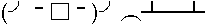
\includegraphics[scale=0.8]{ywz.pdf})

    「啊……毕竟是个小系列。」

    「是这样吧。」

    说着,久美子也把手机拿了出来。上面确实挂着一个活塞型大号的挂件。嘛,反正除了大小不同,上低音号和大号也差不多。要是说了这种话,会惹怒很多乐器的担当者吧。

    「不过你高兴我就放心了。」

    久美子露出羞涩的笑容。总觉得有点害羞,秀一挠了挠头。

    「为了给这个叫我出来的吗?」

    「嗯,是这样怎么了吗?」

    「啊,这样啊。」

    把手机放进口袋里,秀一往夹克上擦了擦手上的汗。久美子似乎对达成目的感到满足了,伸了伸手。

    「那差不多该回去了。」

    「诶,这就回去?」

    被路灯照着的发卡闪闪发亮。对这边的发问,久美子不解地歪着头:

    「嗯?还有什么事吗?」

    「不,倒也不是有事……」

    久美子直直地看着支支吾吾的秀一。周围没有别人。静寂的空间只有两人的声音响起。吹来的冷风掠过秀一的脸颊。从外套的袖口中,露出了久美子苗条的手腕。

    ——但是,还能在一起的时间就只有现在了啊?

    梨子的声音在脑内反复响起。咕噜,喉咙不自觉响了起来。伸出去的手握住了久美子的手腕。那纤细的感觉,不知怎么加快了心脏的跳动。

    「怎么了?」

    想要搞清这边的意图,久美子擡头看向秀一的脸。

    「我啊……」

    话到了喉咙边。什么?——久美子有点颤抖的声音问道。她的唇也呼出白白的雾气。

    「我……」

    从皮肤上传过来、可以感觉到的她手上的脉搏跳动。久美子也带着紧张的神色,等待着这边说话。白色的花瓣进入视线,别着的发夹上面是小小的向日葵。

    为了抑制兴奋的心情,秀一深深地吸了一口气。呼吸的声音震动着自己的鼓膜。

    「其实喜欢……」

    久美子止住了呼吸。沉默的夜晚的空气里,秀一的肩膀因紧张抖着。好热,明明是冬天,热量都集中到皮肤下了。久美子的双眸里映出的光线微微摇动,她的睫毛一上一下地上下跳动着。

    「……喜欢谁?」

    被这么问道后,秀一加大了抓住手腕的力气,直视着久美子的脸,没有移开目光叫道:

    「你啊!」

    感觉失败了一半。秀一对自己说的话感到害羞了,粗暴地用指甲擦拭着自己的嘴。可恶,不知不觉中露出丑态了。久美子放开了抓住的手,像是要隐藏表情一样用双手捂住了自己的脸,她就这么摇摇晃晃着蹲下了。看到预料之外的反应,秀一慌张起来。

    「没事吧?」

    这边问后,久美子轻轻地摇了摇头。她从头发间露出的耳朵,红得像煮熟的番茄一样。

    「有点,心脏砰砰直跳。」

    说完,她脱力地笑了。那脸颊有多红,大概就跟秀一的脸一个颜色吧。站得起来吗?——秀一问道,久美子点了点头。

    「来。」

    她提心吊胆地握住了秀一伸出的手。和秀一不一样,久美子的手是温暖的。

    「今天很温柔呢。」

    「不不,我平时一直这么温柔好吧。」

    「你还说。」

    这么笑着,她的视线落向牵着的手。看着别人的手有什么好玩的吗,秀一总觉得不好意思,轻轻动了动。

    久美子开口:

    「手好凉呢。冷吗?」

    「不,还好。」

    「啊,这个借你。围巾。」

    「哈?」

    「没事啦没事啦。」

    说着,久美子把脖子上卷着的围巾解下。桃粉色的女式围巾,这种可不是男子高中生能戴身上的东西。虽然是这么想的,但难以拒绝这份好意。秀一勉勉强强地把围巾戴上。是因为还残留着久美子的体温吗,肌肤碰到的围巾有点温热。

    「合适。」

    她觉得好笑一样笑了起来,手无意间碰到了秀一的肩膀。这一股劲让秀一不由得把身体倾向了久美子那边。久美子踮起脚尖,进入秀一的视线。她挺直身子贴近秀一耳边,嘴唇过于接近让秀一瞬间定住了。心脏高昂地跳动着,很难意识不到至近距离的她的存在。

    右耳,飘进了久美子的声音。声音混着吐息,让秀一的耳朵痒痒的。洗发水的香味飘进了鼻子。那一句话,确实传到了秀一发硬的耳中。

    「我也喜欢秀一哦。」
\end{document}